\newpage
\chapter{Android Live Wallpaper}
\label{chapter04}

Android Live Wallpaper technology provides animated visual representation capabilities in virtual wallpaper. This type of application does not differ drastically from other Android applications and can perform almost all of their capabilities. Since the virtual wallpaper is always active, it is an ideal candidate for implementing background computing\index{distributed computing}. The following components are required to create an active wallpaper: 1. An XML file that describes the components of the wallpaper; 2. Background module (Android Service); 3. Appropriate permissions to access device resources.

\section{Mobile App Manifest File}

When creating applications for the Android operating system, the approach adopted is to describe the components of the mobile application in a manifest file (AndroidManifest.xml) using XML syntax.

\begin{figure}[h]
\centering
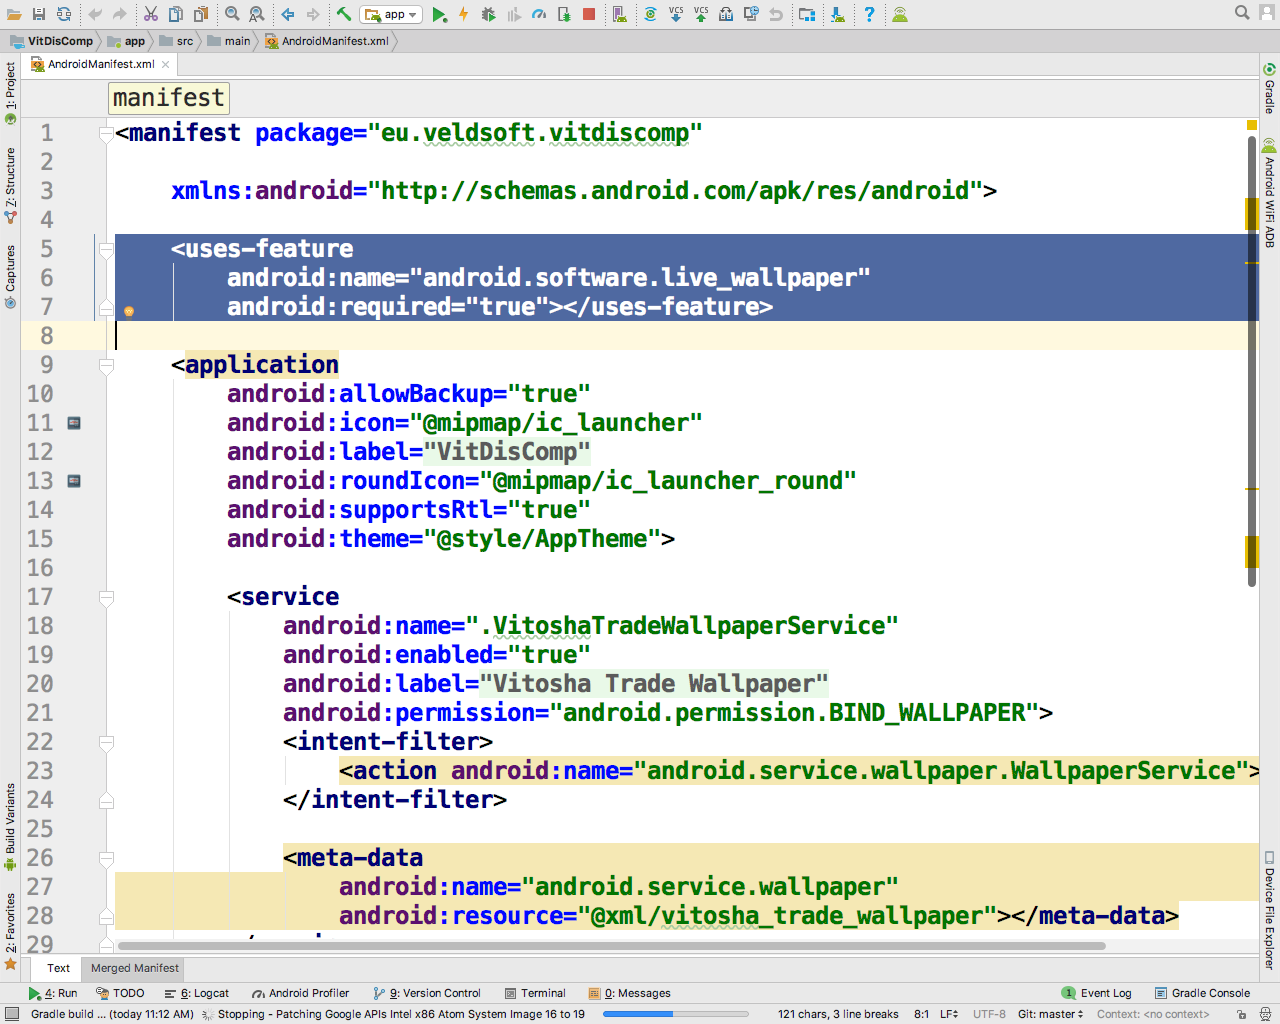
\includegraphics[height=0.45\pdfpageheight]{pic0011}
\caption{Setting the app as active wallpaper}
\label{fig:pic0011}
\end{figure}
\FloatBarrier

To define the application as an active wallpaper application, mark it explicitly in the manifest file (Fig. \ref{fig:pic0011}). The most significant benefit of this definition is that it prevents the application from being installed on devices that do not support live wallpaper rendering capabilities.

\begin{figure}[h]
\centering
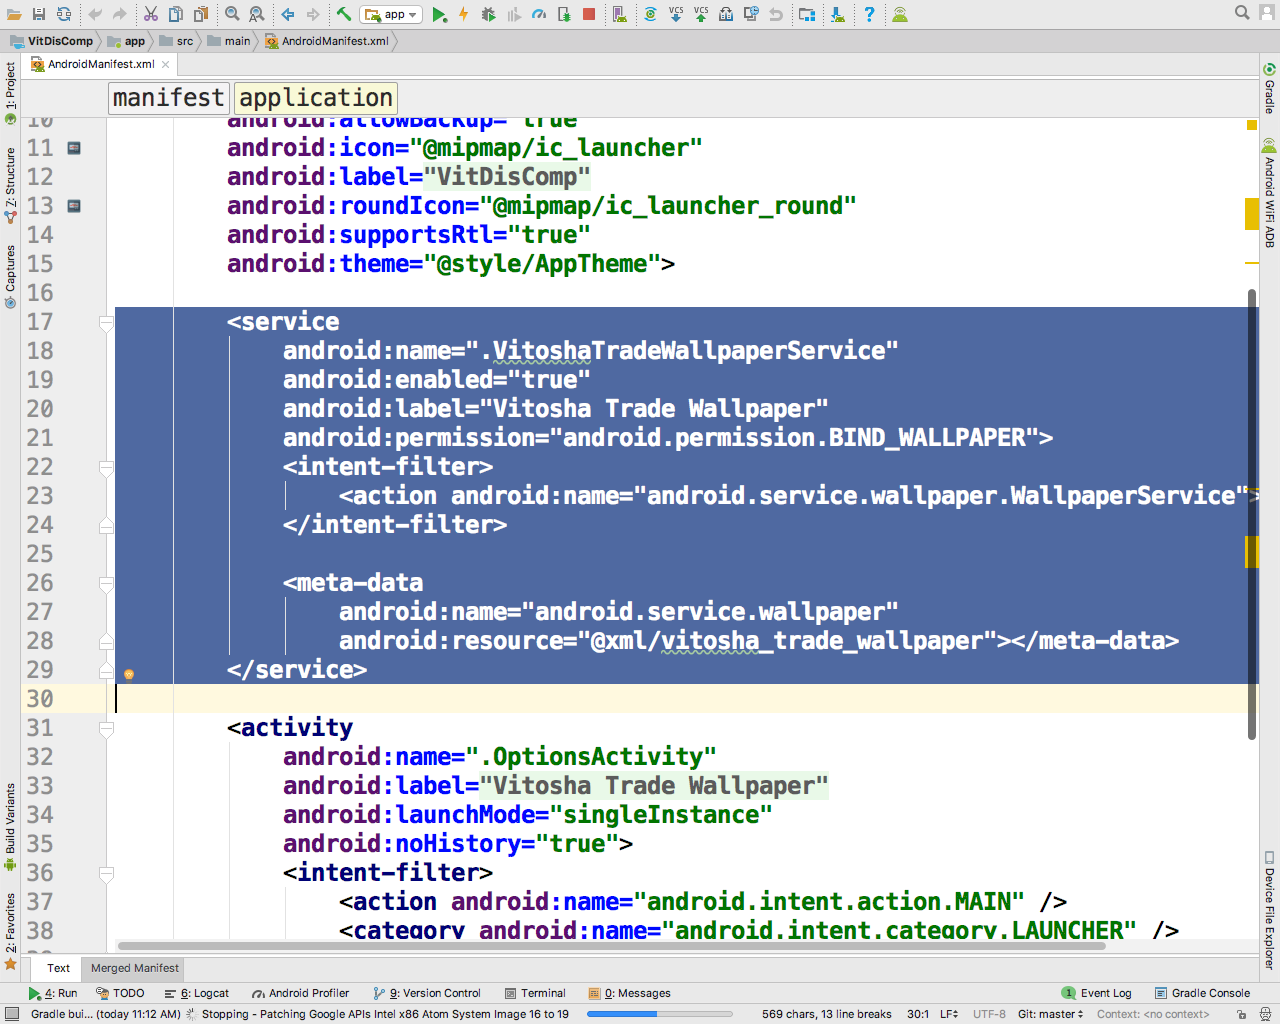
\includegraphics[height=0.45\pdfpageheight]{pic0012}
\caption{Module of type ``service''}
\label{fig:pic0012}
\end{figure}
\FloatBarrier

When an Android application uses very long calculations that are not convenient to perform on the main GUI thread, it is common for a thread to export them to non-GUI modules called "services". The work of the active wallpaper is carried out in just such a module, and for this reason, one has been added to the project (Fig. \ref{fig:pic0012}).

\begin{figure}[h]
\centering
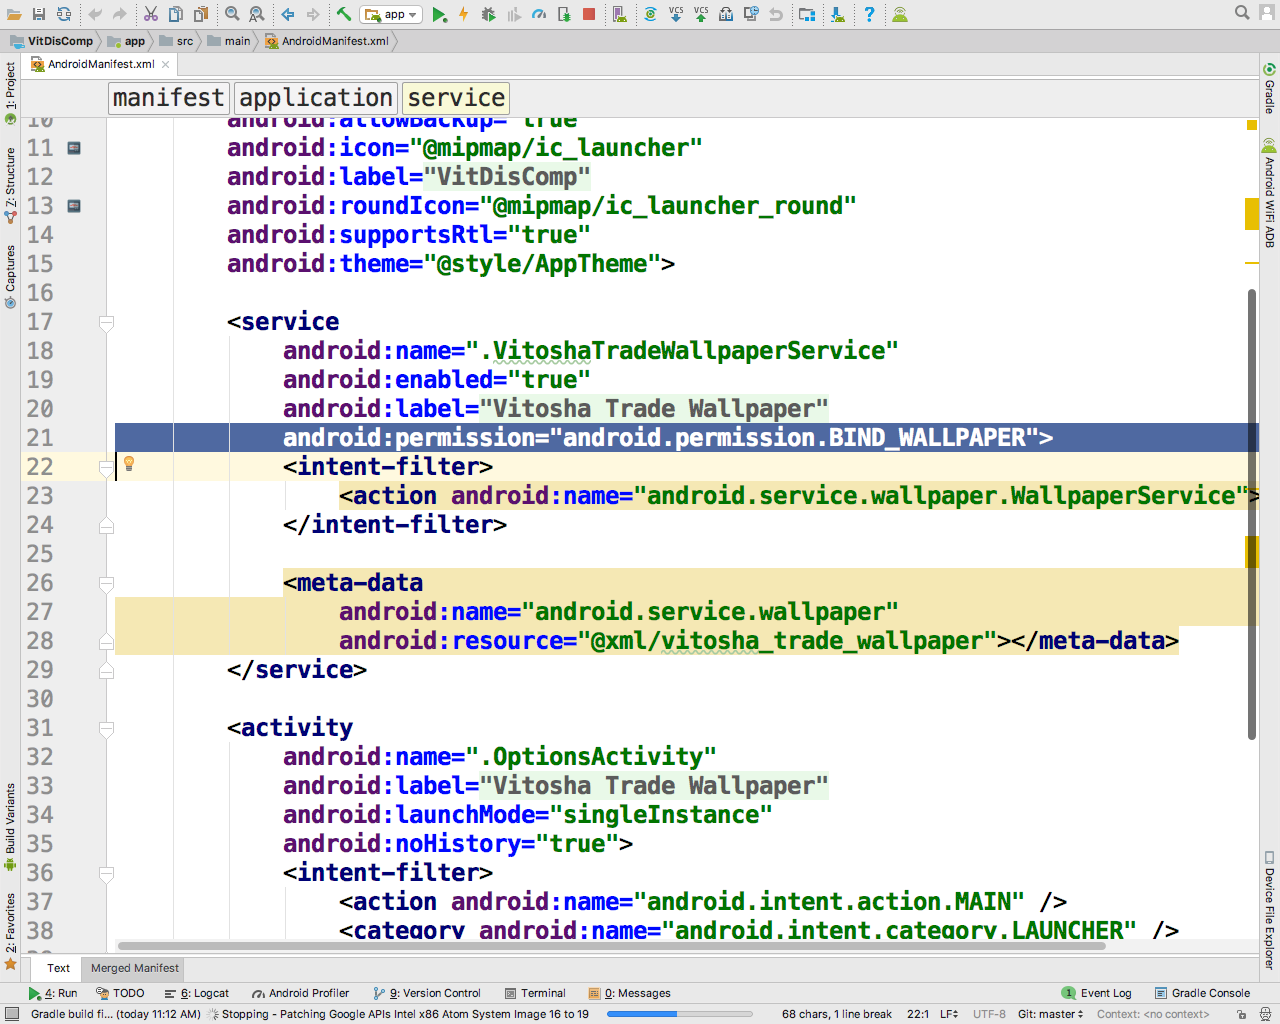
\includegraphics[height=0.45\pdfpageheight]{pic0013}
\caption{Active wallpaper resource access flags}
\label{fig:pic0013}
\end{figure}
\FloatBarrier

The security model requires the user's explicit consent to be obtained for any more specific action, in the case of the active wallpaper, the addition of the android.permission.BIND\_WALLPAPER permission is required (Fig. \ref{fig:pic0013}).

\begin{figure}[h]
\centering
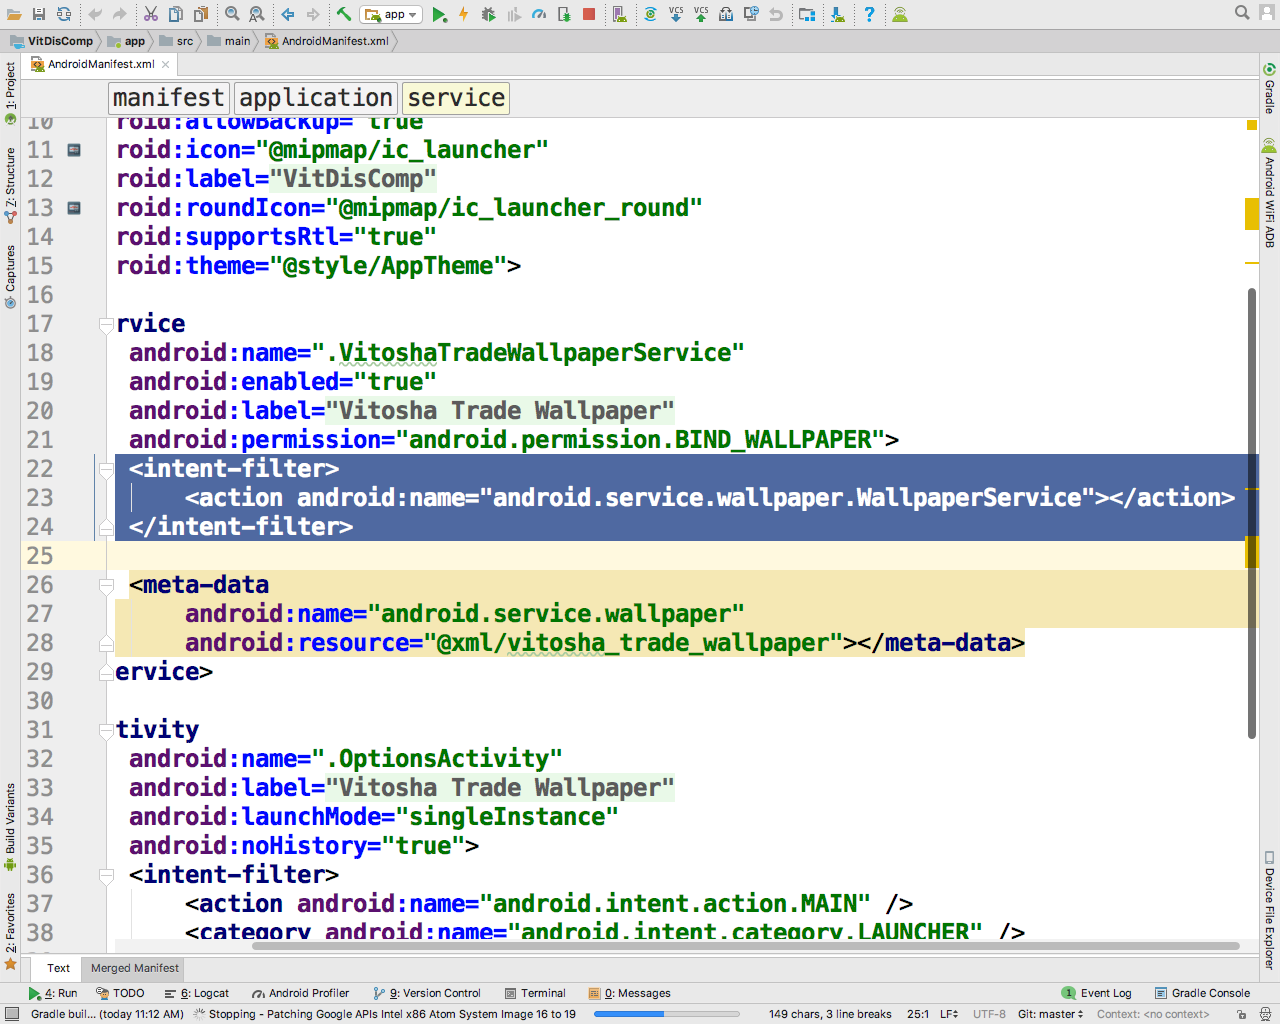
\includegraphics[height=0.45\pdfpageheight]{pic0014}
\caption{Operating system message listening service registration.}
\label{fig:pic0014}
\end{figure}
\FloatBarrier

In addition to the need for permission to use the active wallpaper resources, the service needs to be subscribed to listen for messages from the operating system (Fig \ref{fig:pic0014}).

\begin{figure}[h]
\centering
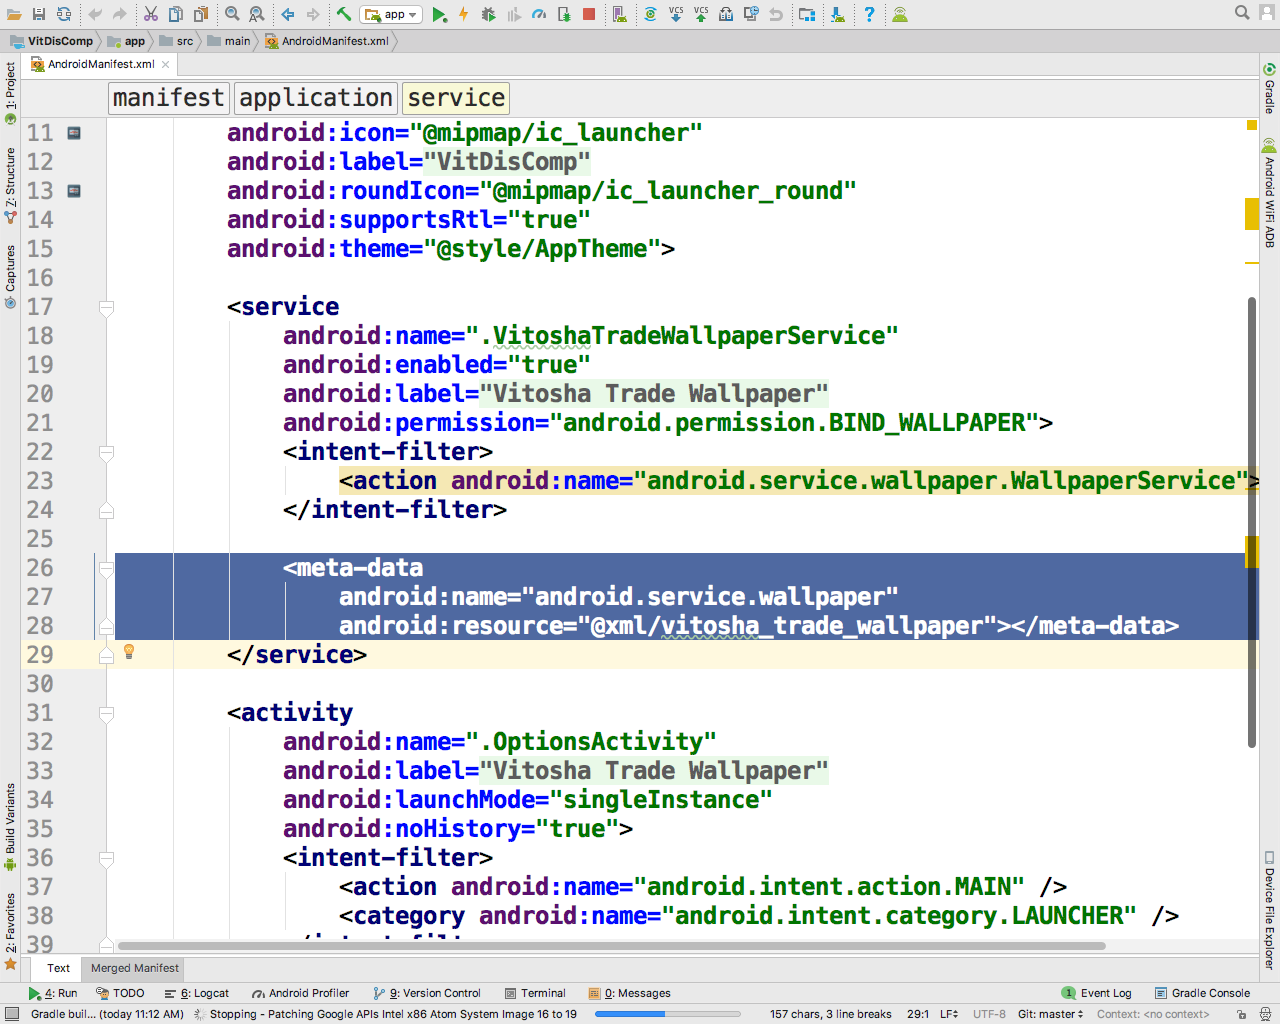
\includegraphics[height=0.45\pdfpageheight]{pic0015}
\caption{Reference to active wallpaper description file}
\label{fig:pic0015}
\end{figure}
\FloatBarrier

The description of the active wallpaper itself is contained in a separate XML file, a reference indicated in the manifest (Fig. \ref{fig:pic0015}).

\begin{figure}[h]
\centering
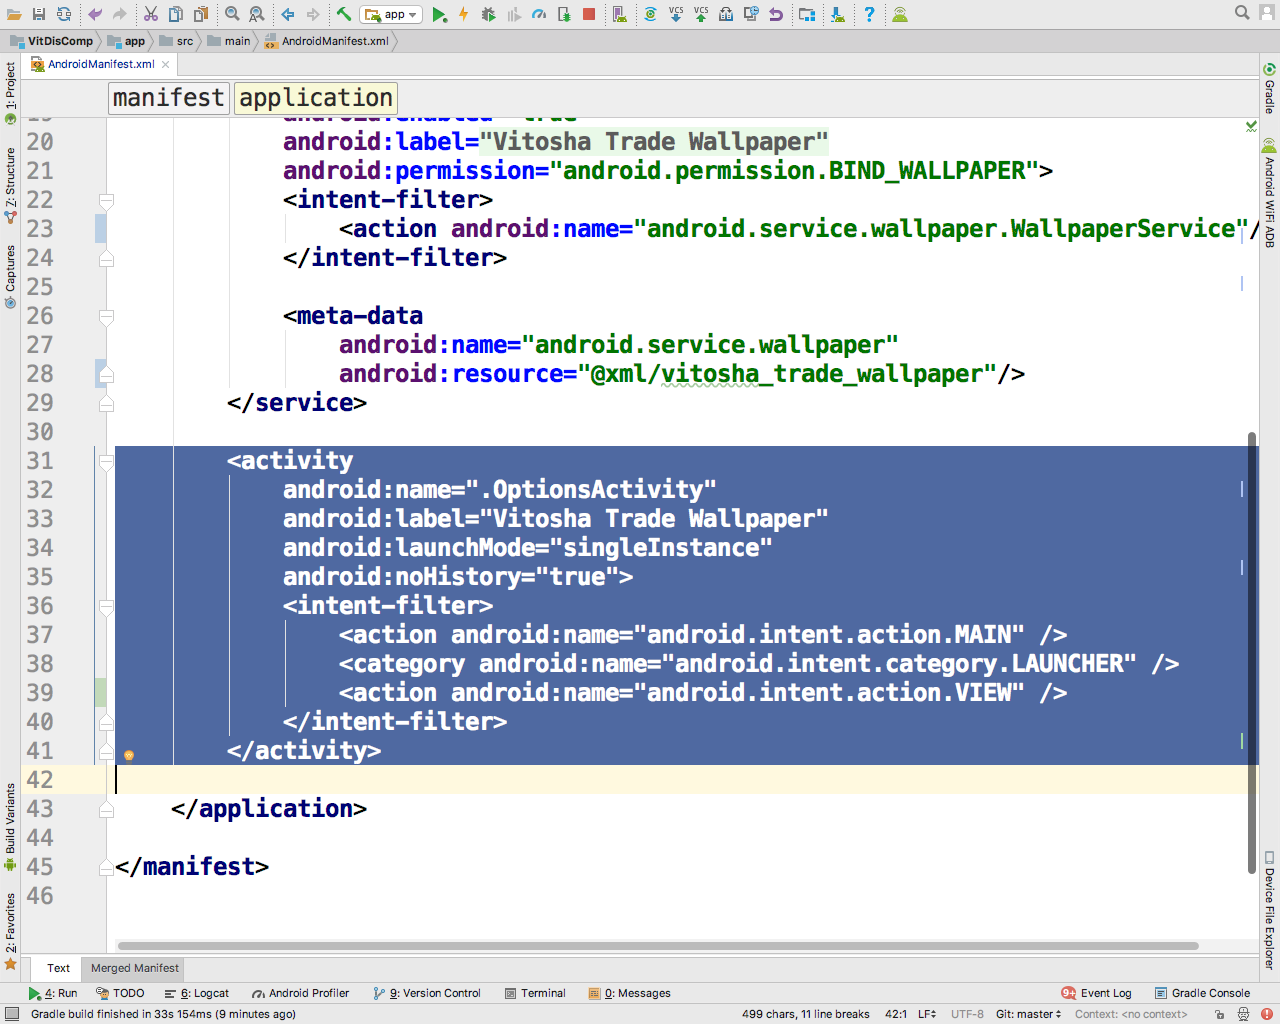
\includegraphics[height=0.45\pdfpageheight]{pic0016}
\caption{Window to set active wallpaper}
\label{fig:pic0016}
\end{figure}
\FloatBarrier

The last component in such an application is a window (Android Activity) to be launched by the operating system and serve to establish the active wallpaper (Fig. \ref{fig:pic0016}). In this case, the possibility is used that this launch window also combines the functions of a window with options (Preference Activity).

\begin{figure}[h]
\centering
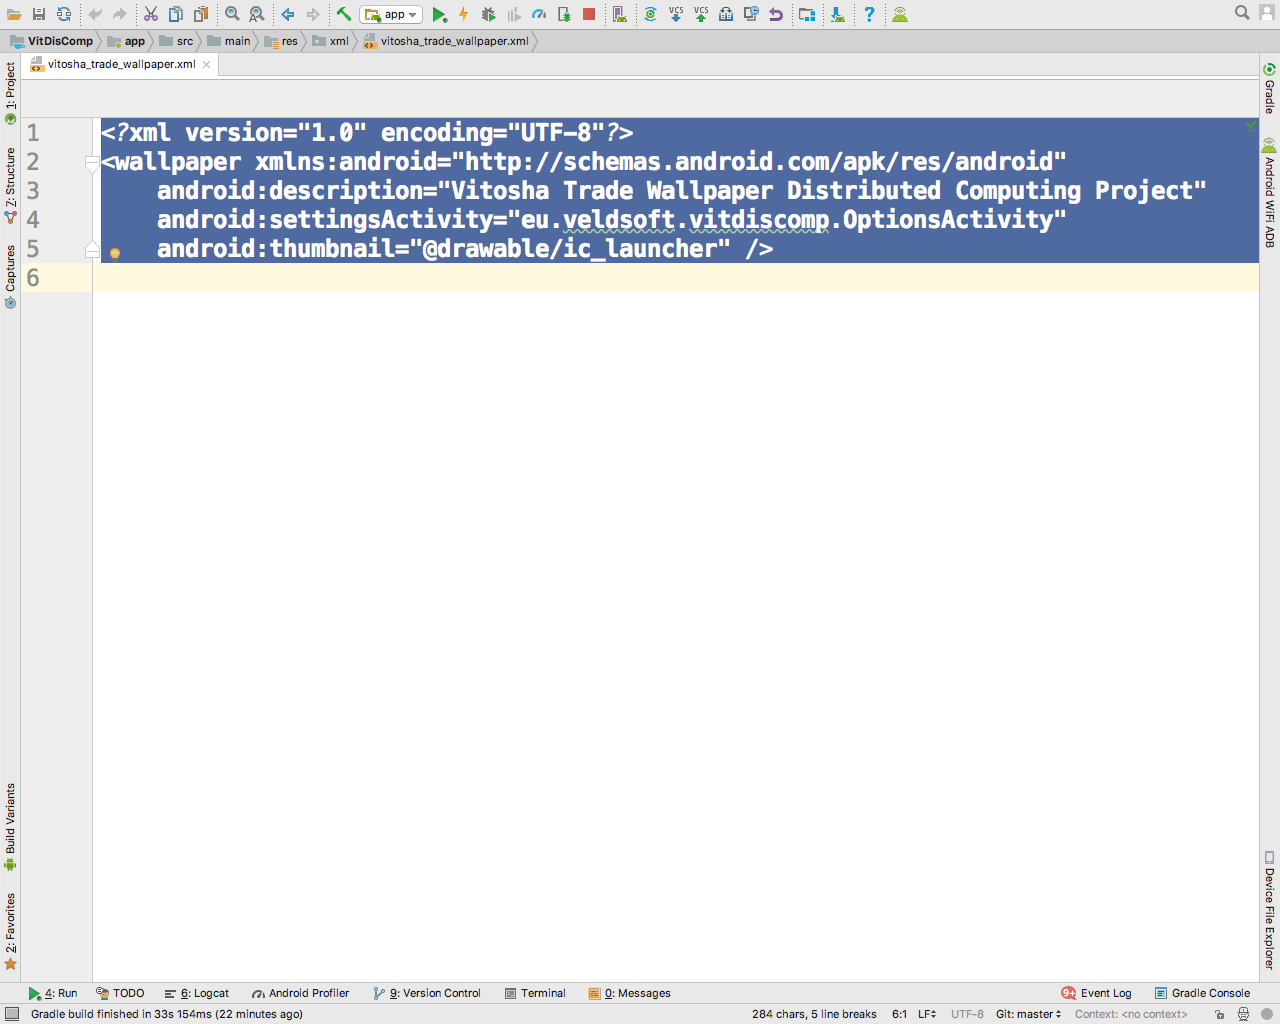
\includegraphics[height=0.45\pdfpageheight]{pic0017}
\caption{XML wallpaper description file}
\label{fig:pic0017}
\end{figure}
\FloatBarrier

As already mentioned, the active wallpaper is described in a separate XML file, which contains a short annotation of the application, a preview, a thumbnail icon, and the name of the settings window (Fig. \ref{fig:pic0017}).

\section{Settings Screen}

Since the active wallpaper will also have a secondary task of visualizing the progress of calculations, it is reasonable to create a settings window for it.

\begin{figure}[h]
\centering
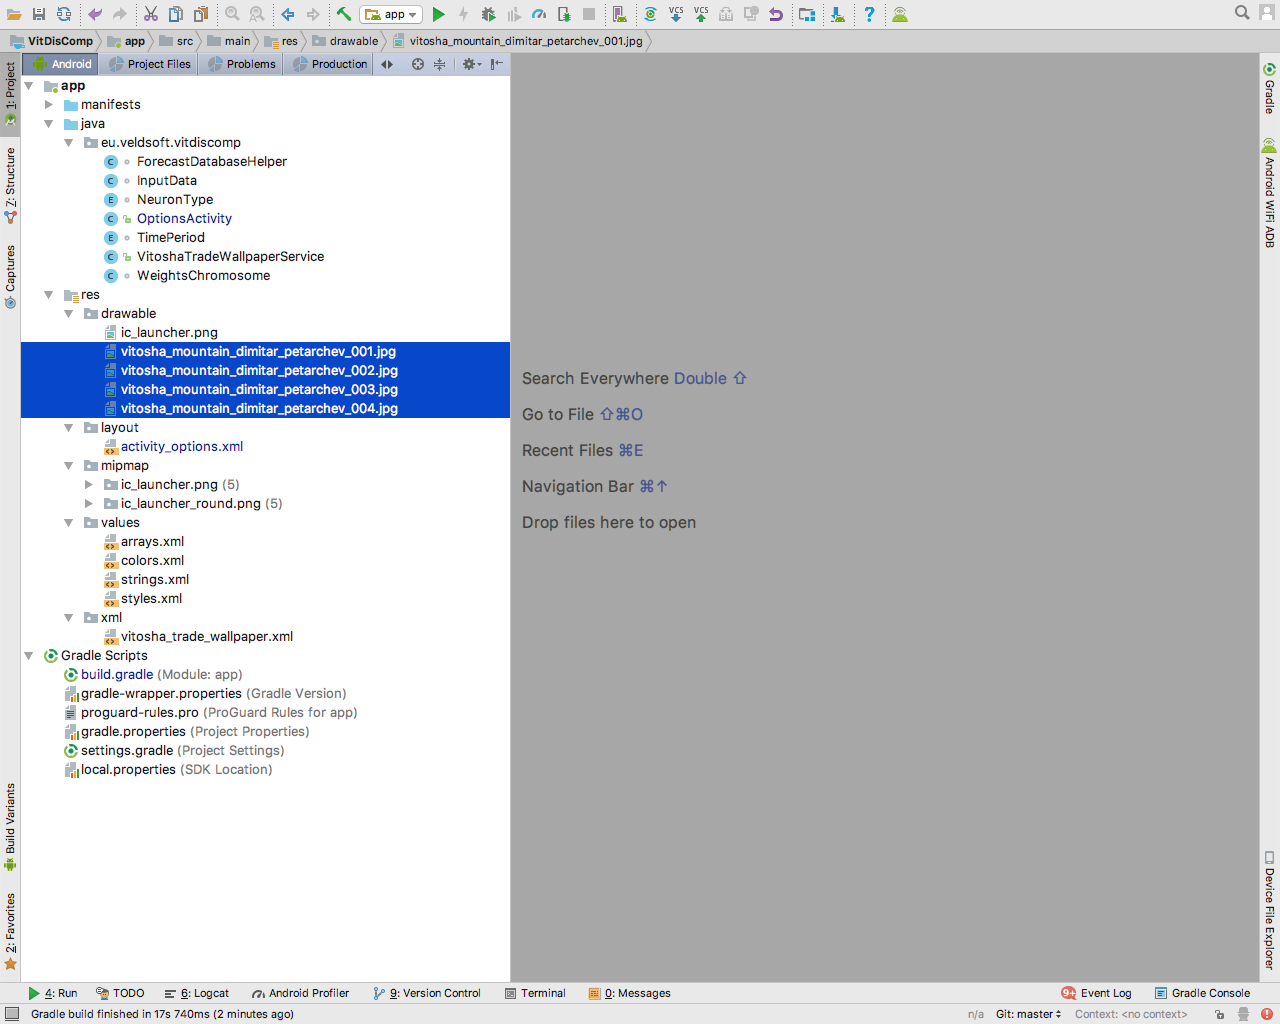
\includegraphics[height=0.45\pdfpageheight]{pic0018}
\caption{Graphic files containing photographs of Vitosha Mountain near the city of Sofia, Bulgaria}
\label{fig:pic0018}
\end{figure}
\FloatBarrier

As a visual representation, the simplest possible option has been chosen. Several photographs of the Vitosha mountain are visualized in the form of segments with the dimensions of the screen of the mobile device (Fig. \ref{fig:pic0018}). Three translucent areas visualize information about the financial time series (code and period), a bar chart about the input and output data, and the current state of the artificial neural network\index{artificial neural networks} (Fig. \ref{fig:pic0019} ).

\begin{figure}[h]
\centering
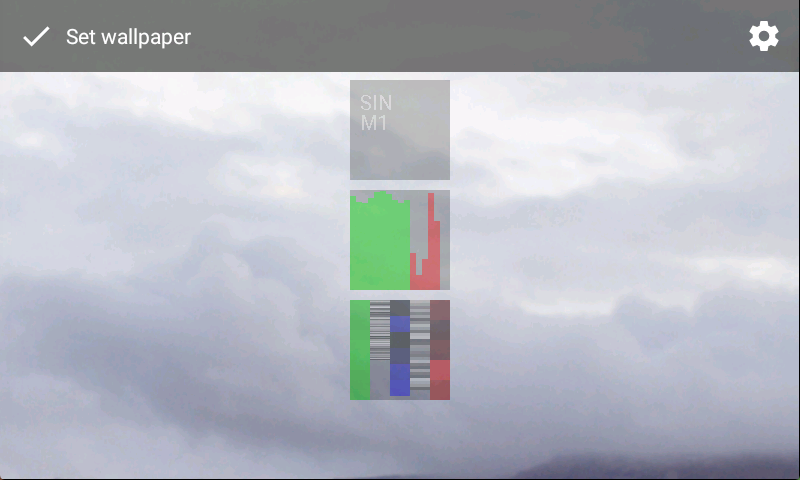
\includegraphics[width=1.0\linewidth]{pic0019}
\caption{Visual representation of information from calculations}
\label{fig:pic0019}
\end{figure}
\FloatBarrier

The live wallpaper settings provide position and size controls for the three visual areas. They also added initial settings for device load level and whether to enable active wallpaper (Fig \ref{fig:pic0020}).

\begin{figure}[h]
\centering
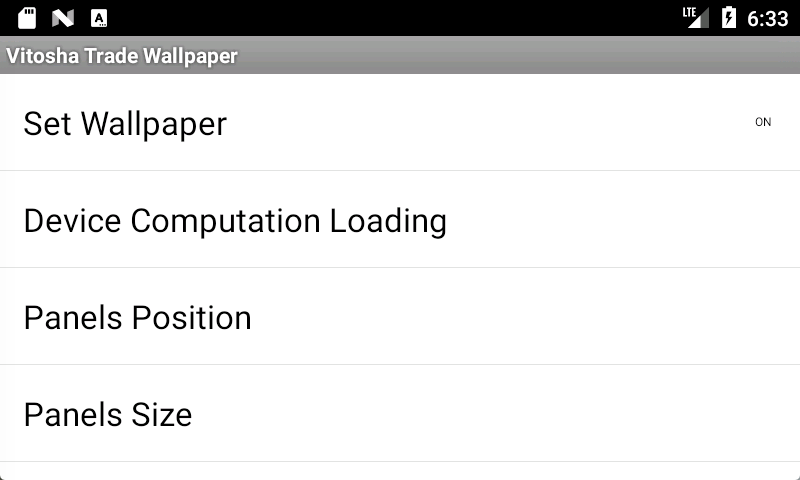
\includegraphics[width=1.0\linewidth]{pic0020}
\caption{Initial set of settings}
\label{fig:pic0020}
\end{figure}
\FloatBarrier

Each window in Android is described with its layout file and Java code file. A GUI descriptor file uses XML and is very similar to composing a web page. When designing a settings screen, one of the most valuable tools in the Android operating system is Shared Preferences. They allow the state of visual components to be directly stored in the device in the form of key-value pairs and then programmatically used for this information.

\subsection{Description of the user interface in the form of XML files}

\begin{figure}[h]
\centering
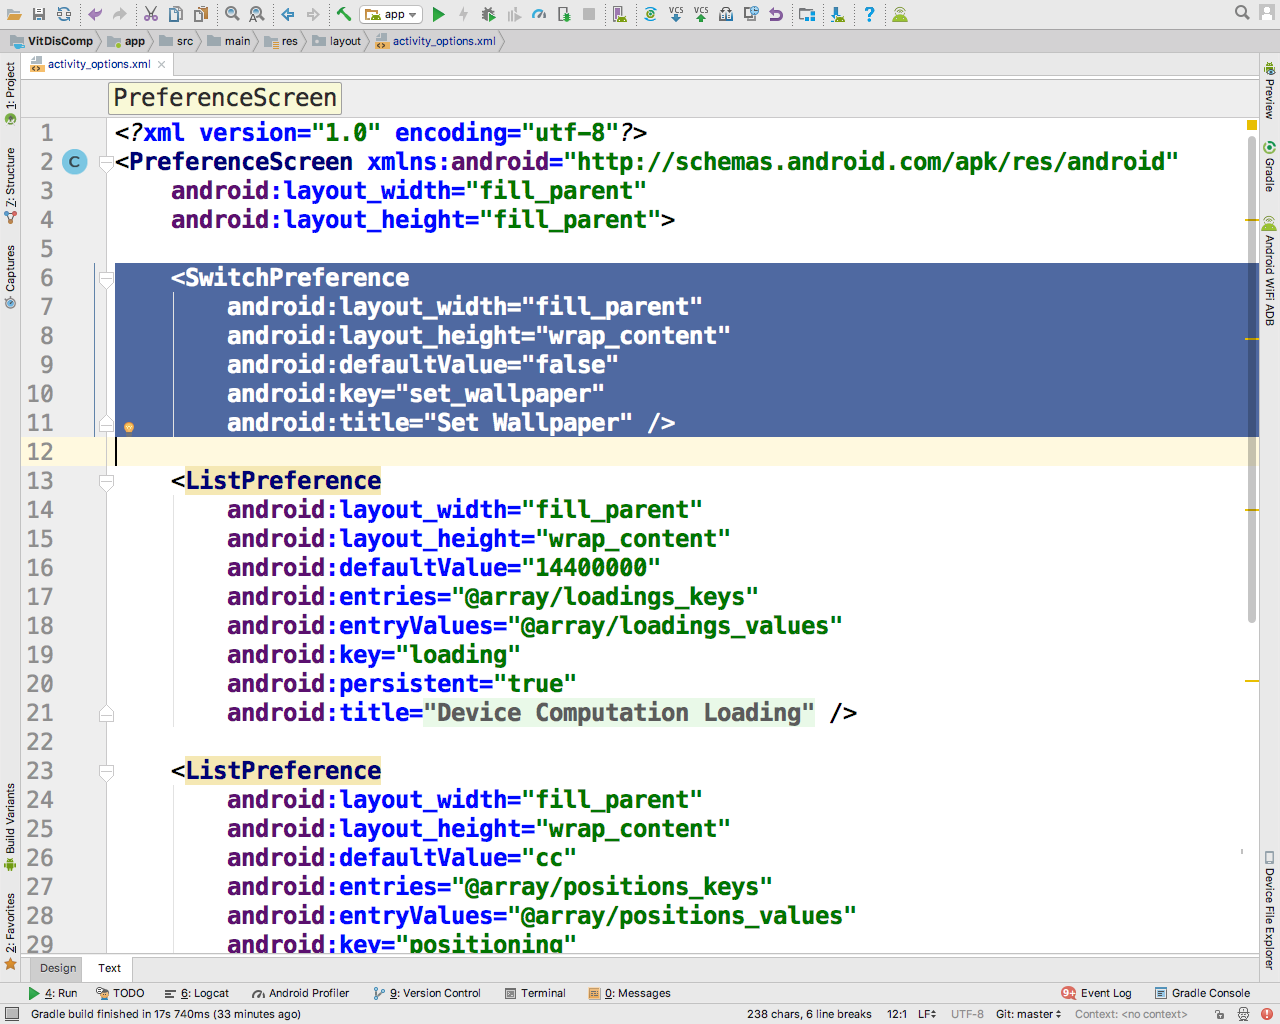
\includegraphics[height=0.45\pdfpageheight]{pic0021}
\caption{Visual component to turn wallpaper on and off}
\label{fig:pic0021}
\end{figure}
\FloatBarrier

First, there is a visual component for turning on and off the active wallpaper. When the switch is in the ON state, the active wallpaper is started, and when it is in the OFF position, the active wallpaper is disabled (Fig. \ref{fig:pic0021}).

\begin{figure}[h]
\centering
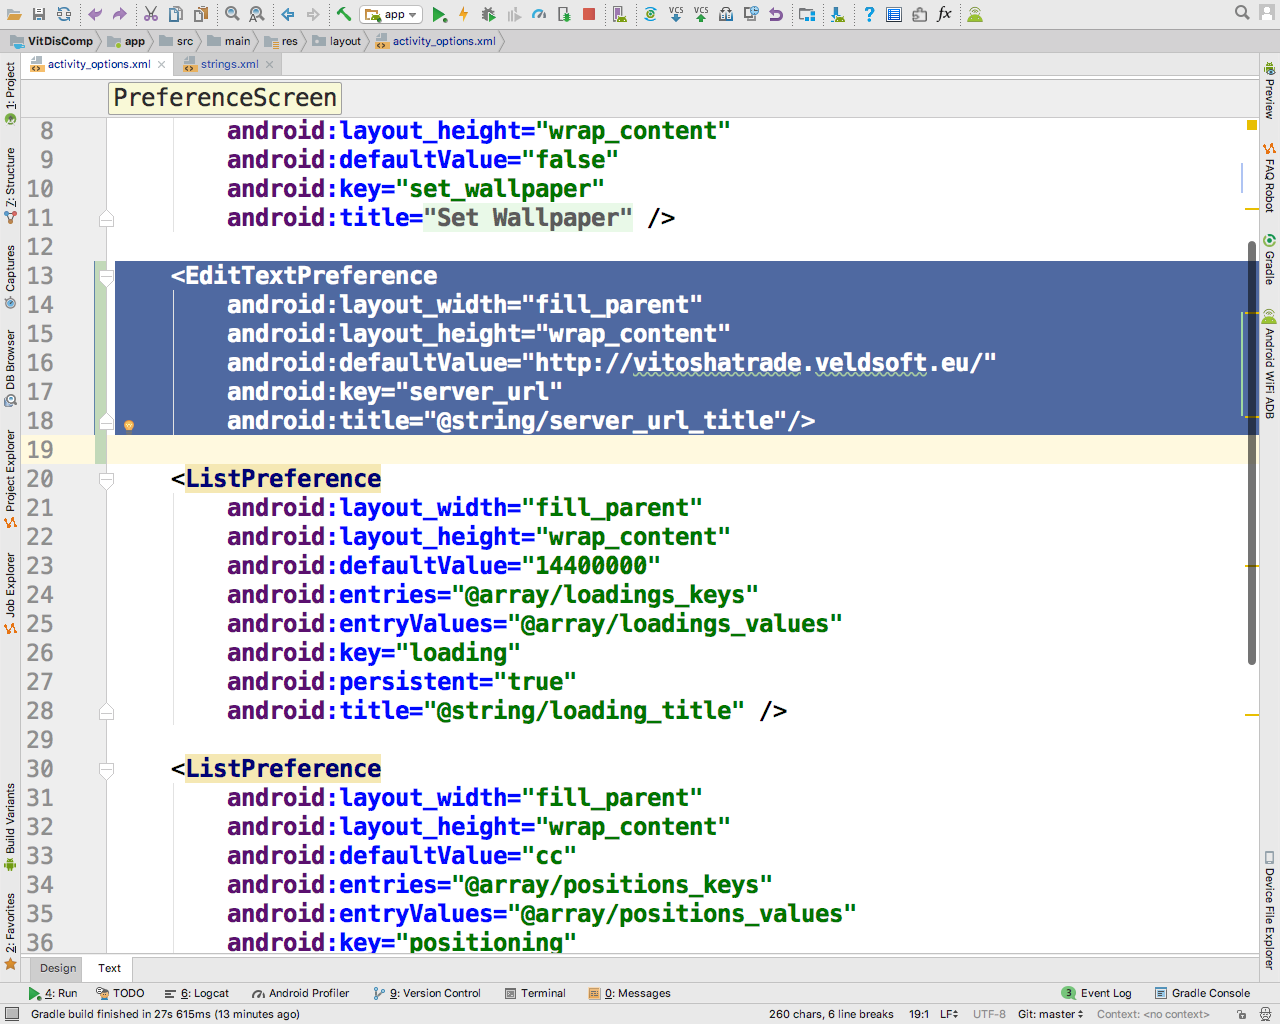
\includegraphics[height=0.45\pdfpageheight]{pic0154}
\caption{Visual Component for Specifying a Server URL}
\label{fig:pic0154}
\end{figure}
\FloatBarrier

Since the mobile application pulls the time series information from a remote web server, it is appropriate for the user to be able to set the URL of the server being worked with (Fig. \ref{fig:pic0154}). This option allows traffic to be redirected to other servers after the application is installed on users' mobile devices.

\begin{figure}[h]
\centering
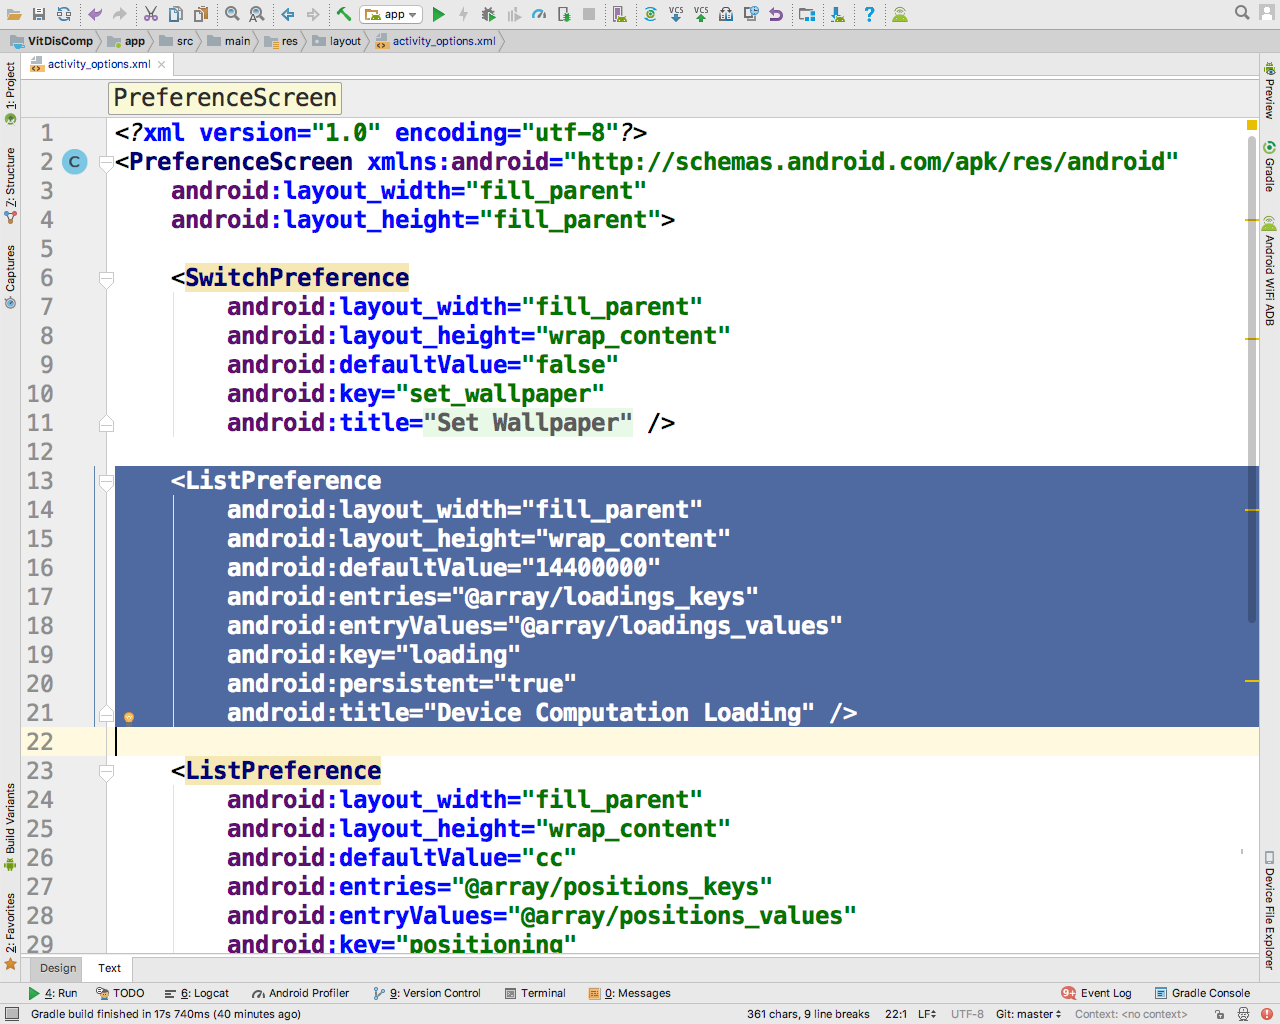
\includegraphics[height=0.45\pdfpageheight]{pic0022}
\caption{Visual load adjustment component}
\label{fig:pic0022}
\end{figure}
\FloatBarrier

A list of predefined values is used to load the device when performing the background calculations (Fig. \ref{fig:pic0022}).

\begin{figure}[h]
\centering
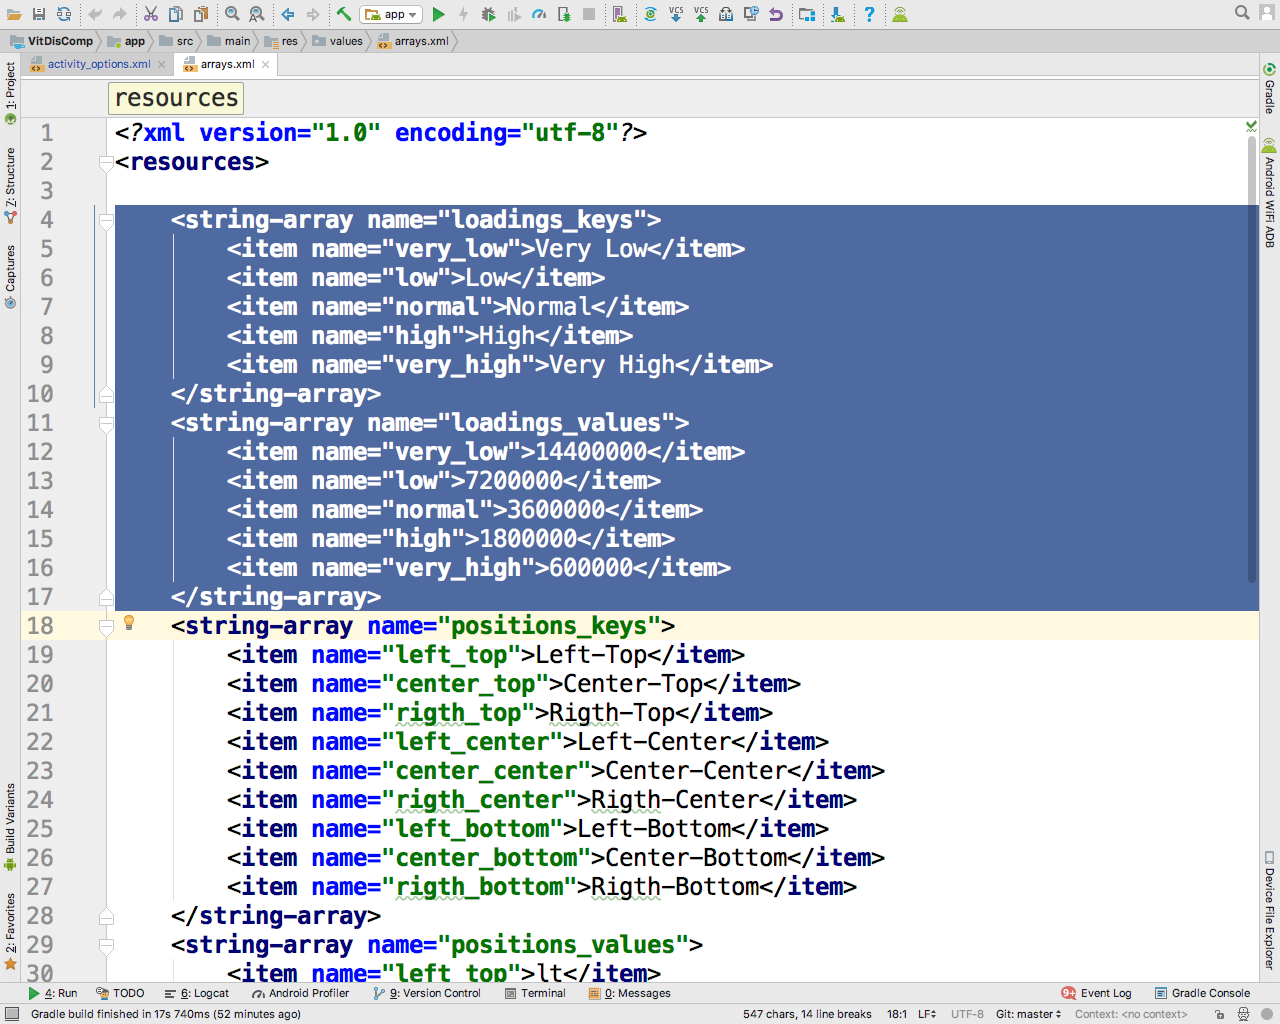
\includegraphics[height=0.45\pdfpageheight]{pic0023}
\caption{System Load Values}
\label{fig:pic0023}
\end{figure}
\FloatBarrier

When designing the Android system, one of the main goals was to separate the graphical interface from the data as much as possible. This is precisely why the load level values are exported in a separate resource (Fig. \ref{fig:pic0023}).

\begin{figure}[h]
\centering
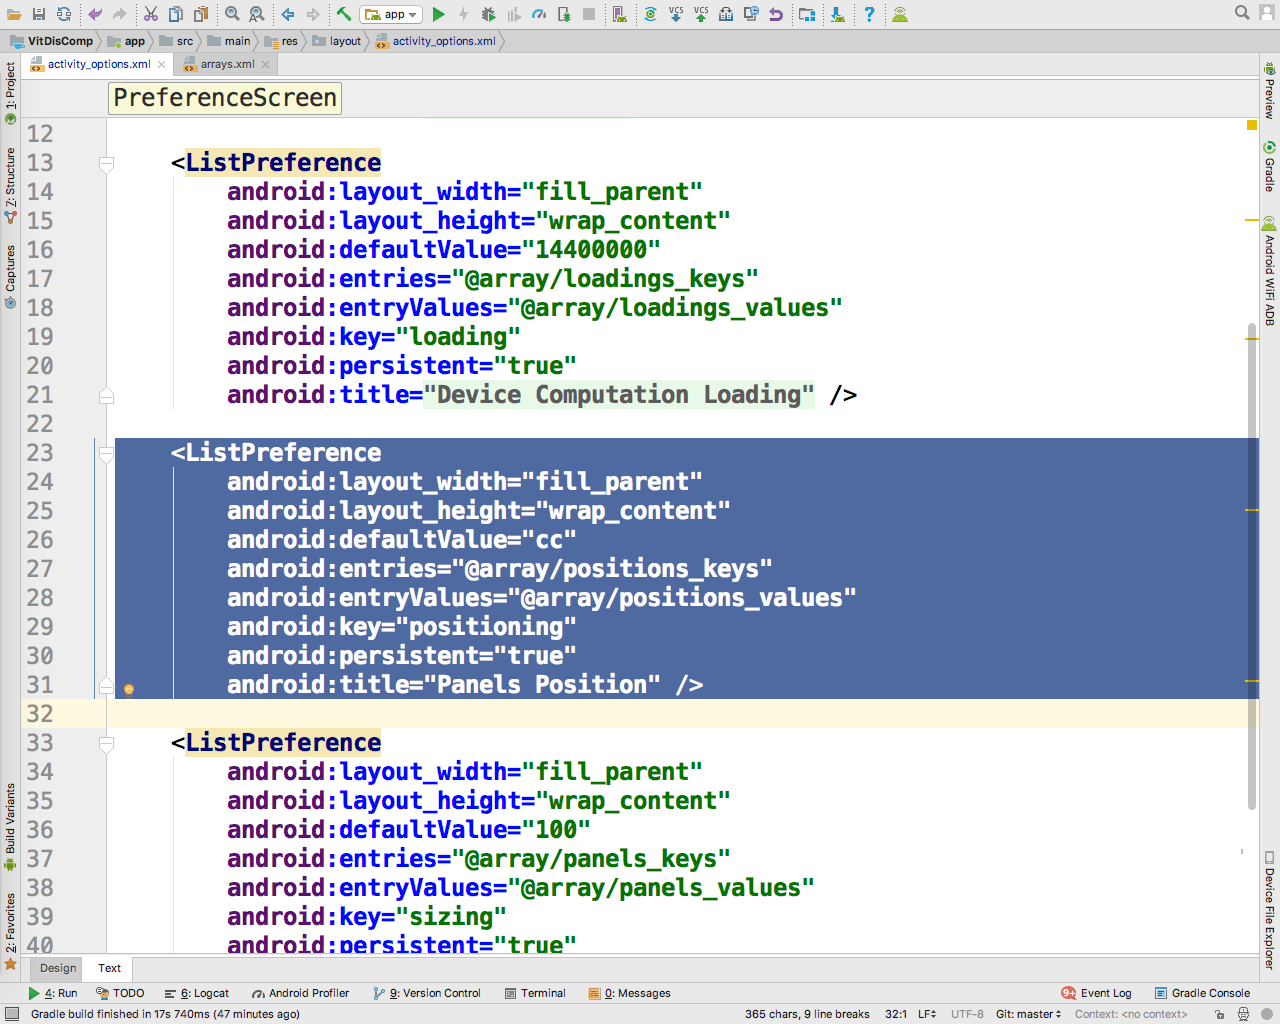
\includegraphics[height=0.45\pdfpageheight]{pic0024}
\caption{Positioning of visual presentation areas}
\label{fig:pic0024}
\end{figure}
\FloatBarrier

The positioning of the visual representation areas is also adjusted by selecting values from a list (Fig. \ref{fig:pic0024}).

\begin{figure}[h]
\centering
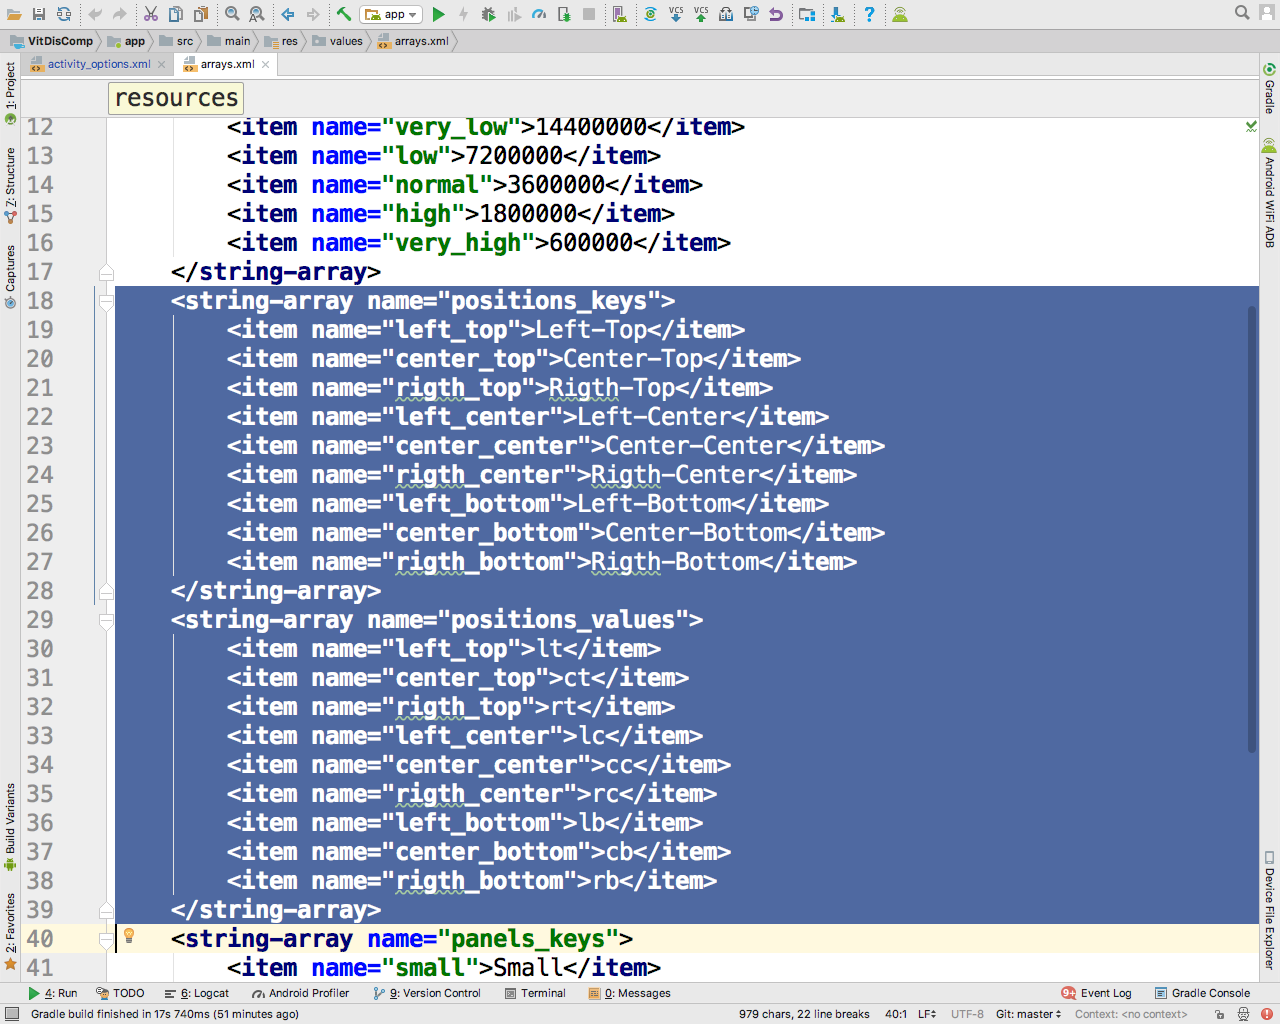
\includegraphics[height=0.45\pdfpageheight]{pic0025}
\caption{Position values for visual representation areas}
\label{fig:pic0025}
\end{figure}
\FloatBarrier

Analogously to the load level values, the list of possible positions of the visual representation areas is exported in a separate resource file (Fig. \ref{fig:pic0025}).

\begin{figure}[h]
\centering
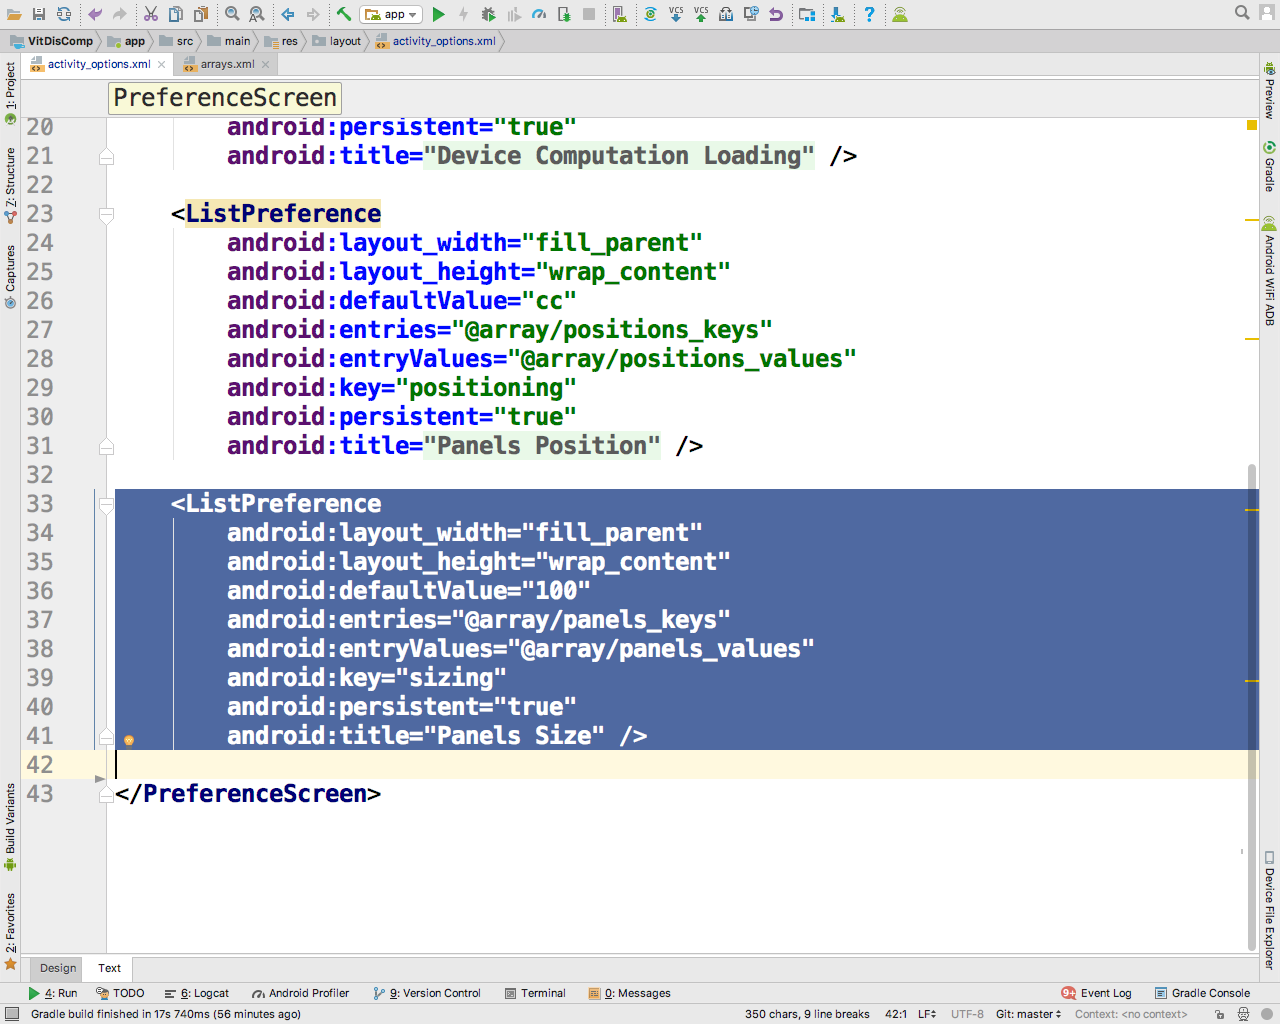
\includegraphics[height=0.45\pdfpageheight]{pic0026}
\caption{Size of visual representation areas}
\label{fig:pic0026}
\end{figure}
\FloatBarrier

Of the initial characteristics, the last is the size of the areas for the visual presentation of information (Fig. \ref{fig:pic0026}).

\begin{figure}[h]
\centering
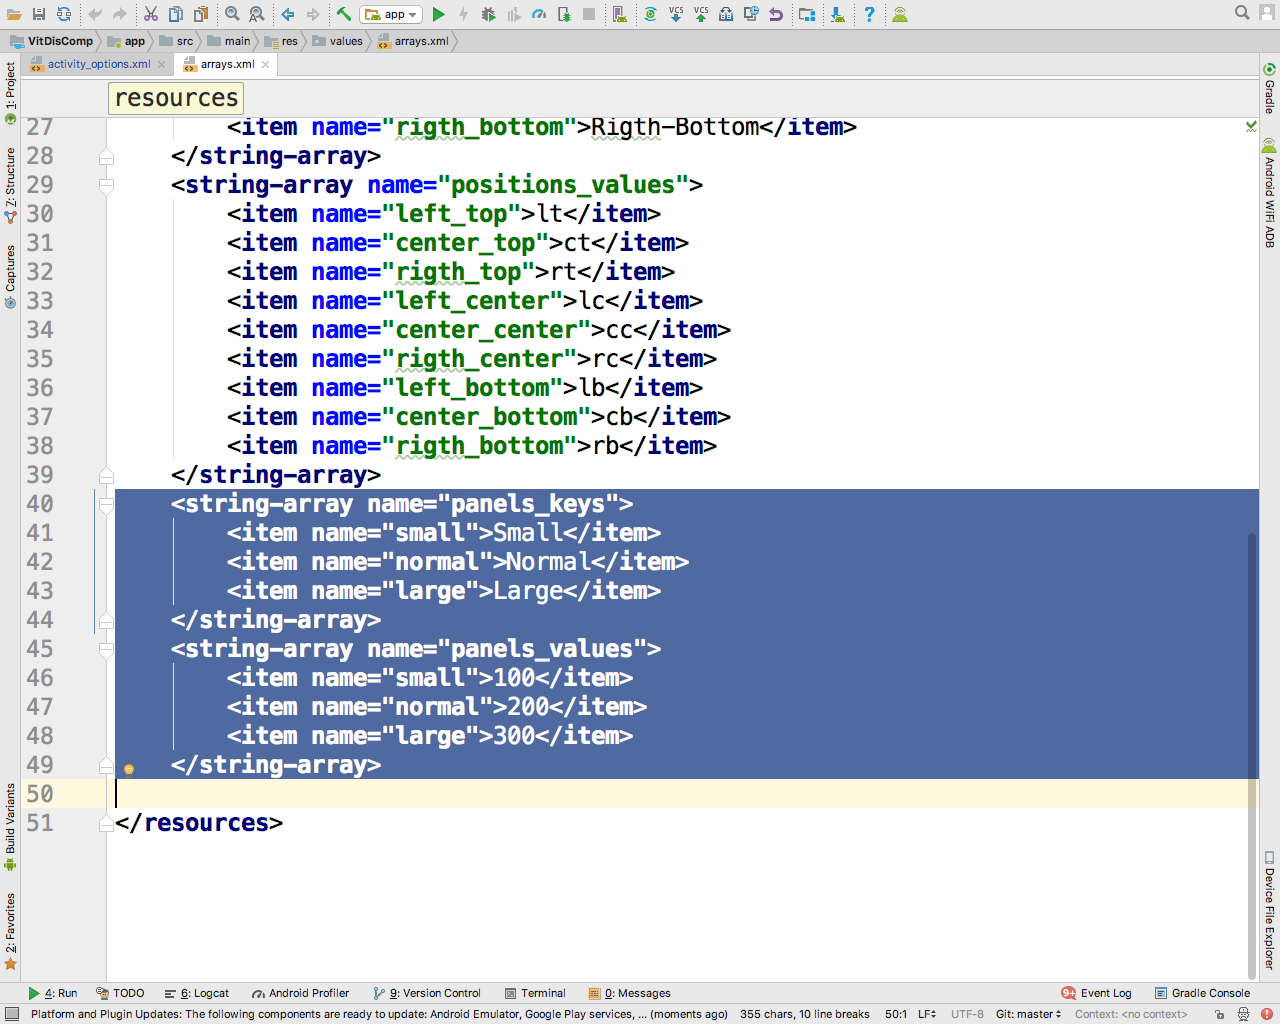
\includegraphics[height=0.45\pdfpageheight]{pic0027}
\caption{Size values for visual representation areas}
\label{fig:pic0027}
\end{figure}
\FloatBarrier

Areas for the visual representation of information are available in three sizes small, medium, and large (Fig. \ref{fig:pic0027}).

\subsection{Interface Control Program Code}

Events raised by the GUI are intercepted in specially written Java functions so that when they are activated, the necessary programmatic actions are performed. Only two events are caught for the settings screen - create and pause.

\begin{figure}[h]
\centering
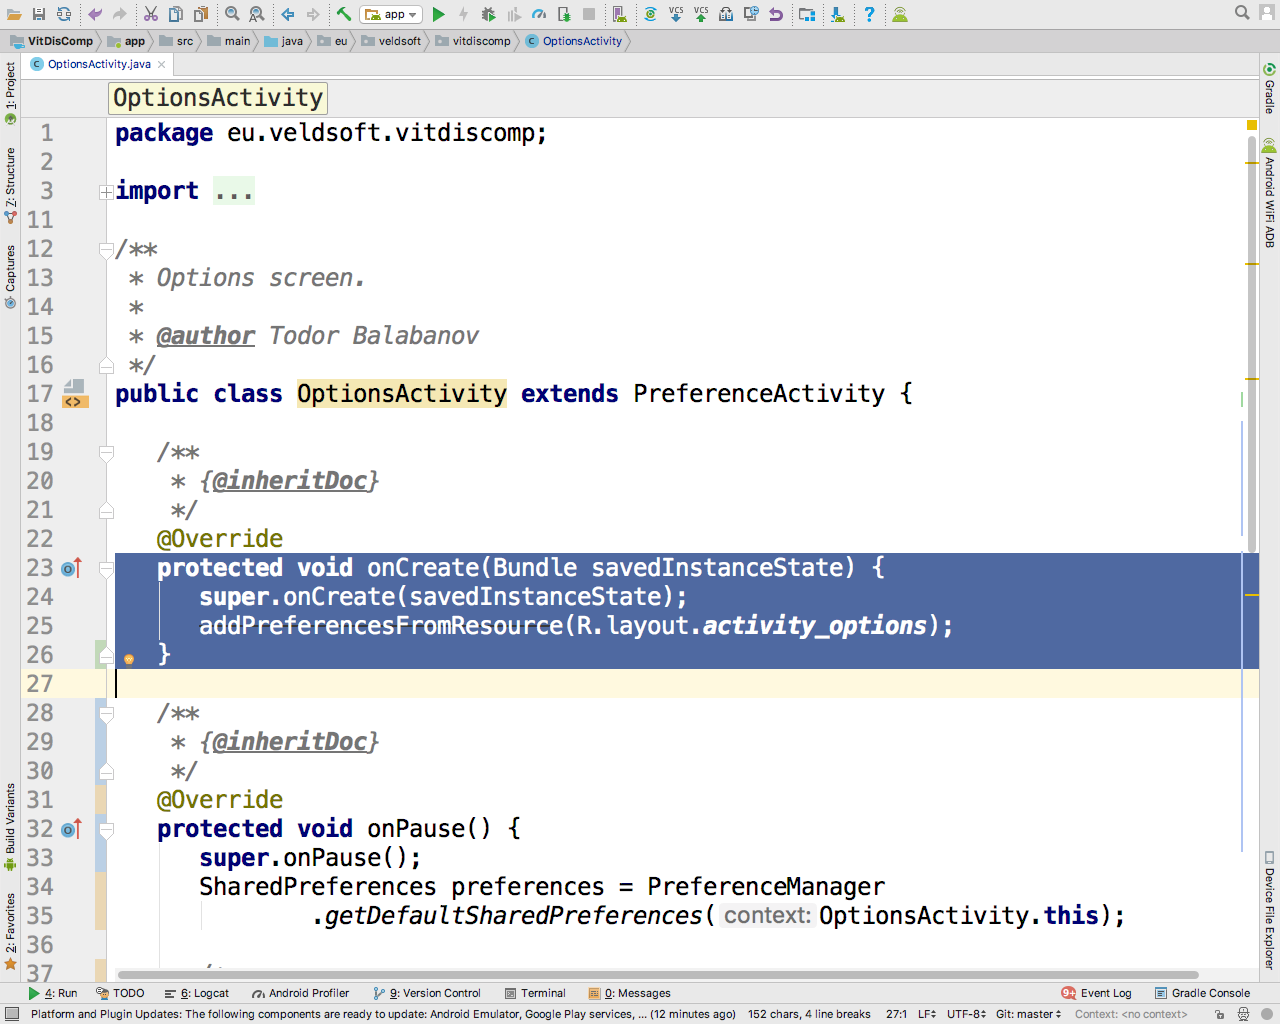
\includegraphics[height=0.45\pdfpageheight]{pic0028}
\caption{Window creation event}
\label{fig:pic0028}
\end{figure}
\FloatBarrier

The create event aims to transform the XML description of the interface into visual components visible to the user (Fig. \ref{fig:pic0028}).

\begin{figure}[h]
\centering
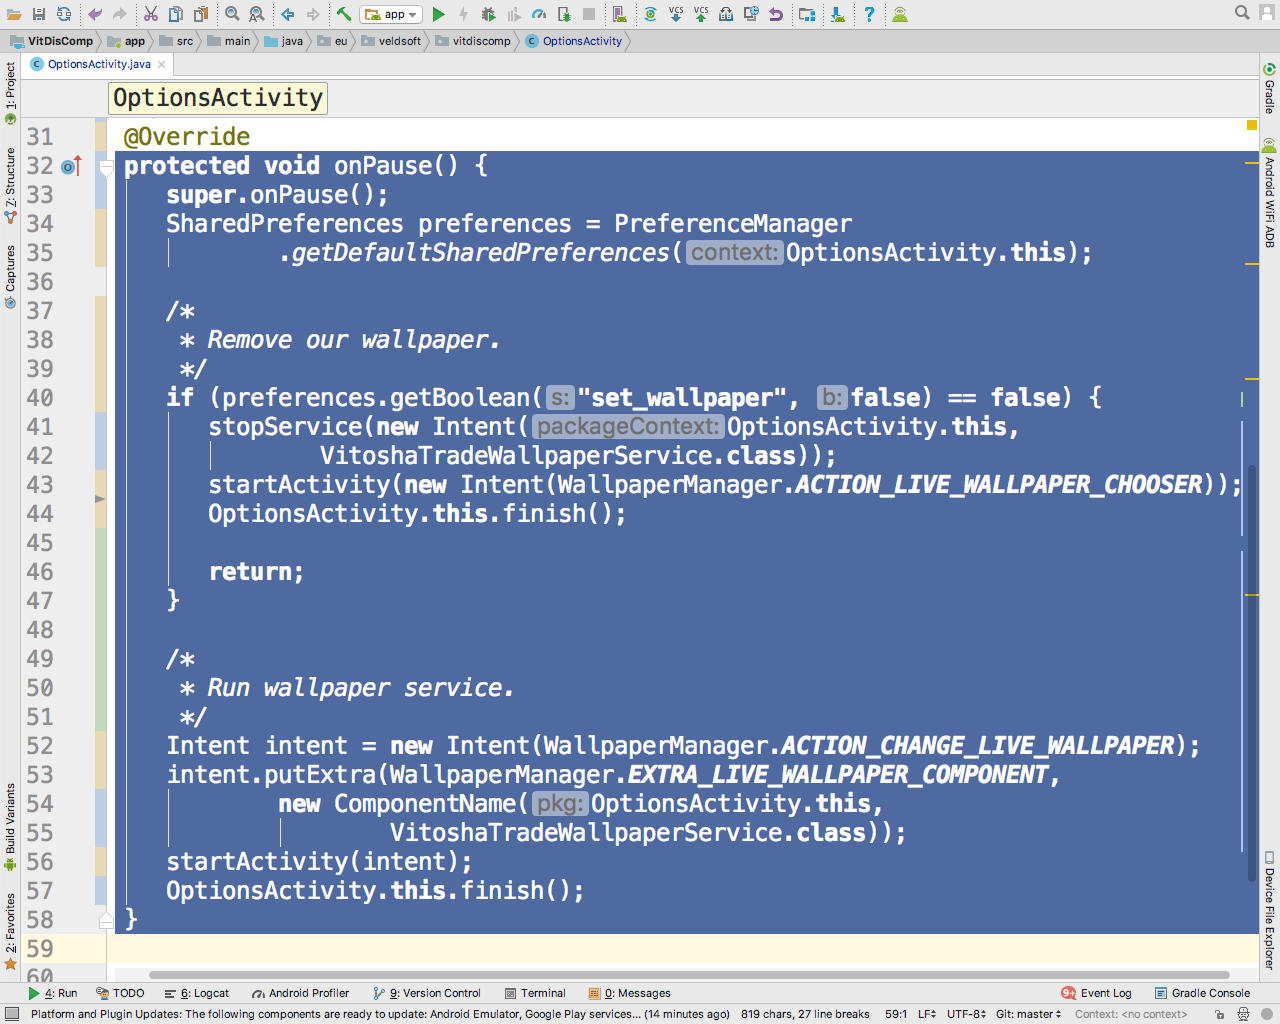
\includegraphics[height=0.45\pdfpageheight]{pic0029}
\caption{Window Pause Event}
\label{fig:pic0029}
\end{figure}
\FloatBarrier

The pause event only decides whether the active wallpaper should be started or stopped (Fig. \ref{fig:pic0029}).

\section{Background Calculation}

Long-running calculations that do not require a graphical user interface are carried out in modules called "services". When it comes to active wallpaper, it is necessary to write its class that inherits from the WallpaperService class (Fig. \ref{fig:pic0030}).

\begin{figure}[h]
\centering
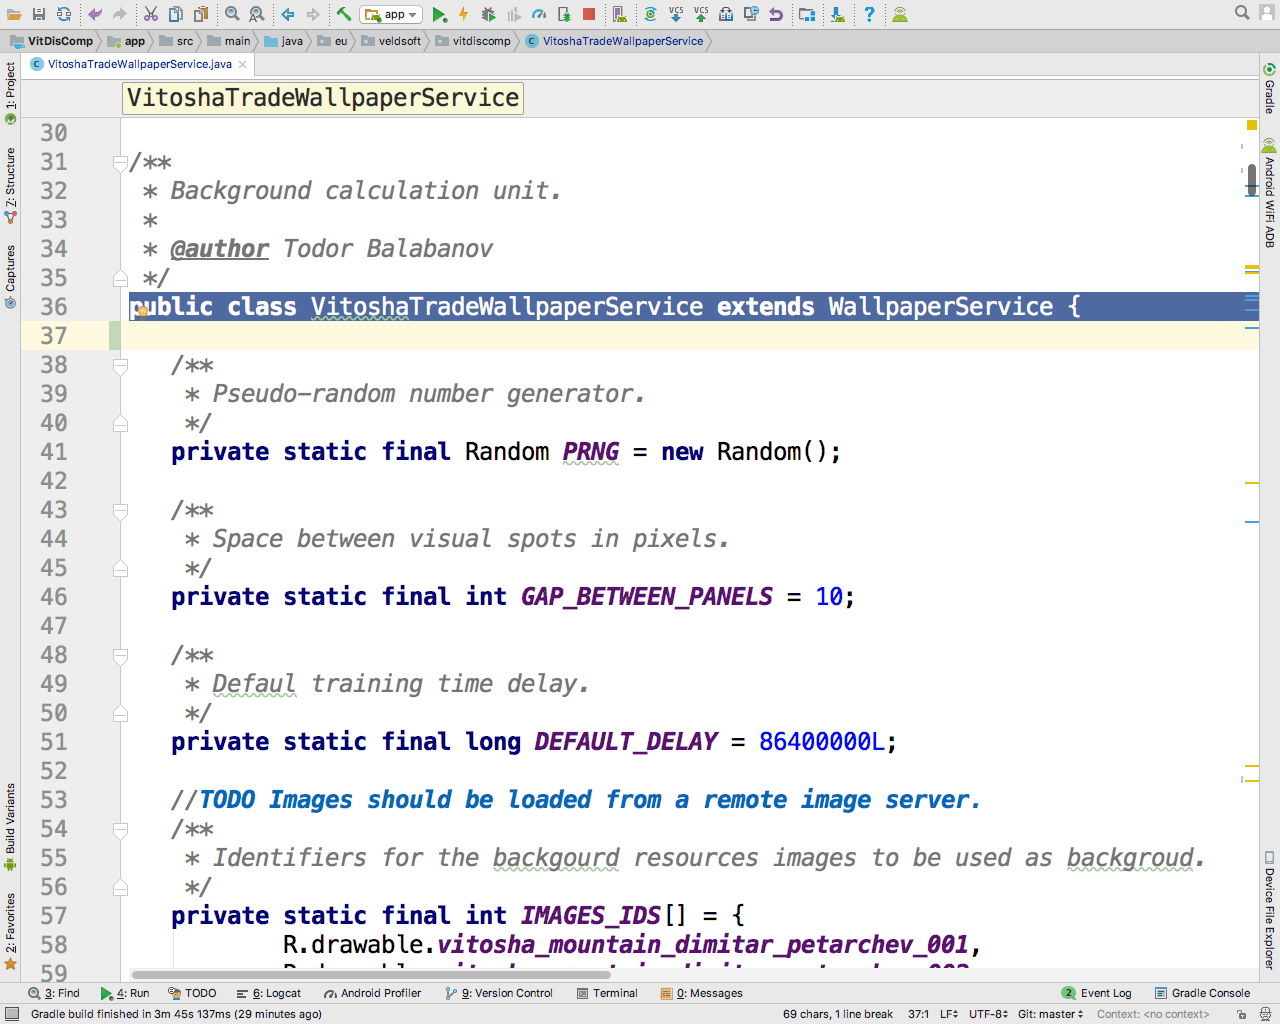
\includegraphics[height=0.45\pdfpageheight]{pic0030}
\caption{Inheriting WallpaperService}
\label{fig:pic0030}
\end{figure}
\FloatBarrier

A group of constants helps generate random numbers, specify a distance between the visual representation areas, and an implied value for the time between two separate runs of the training algorithm (Fig. \ref{fig:pic0031}).

\begin{figure}[h]
\centering
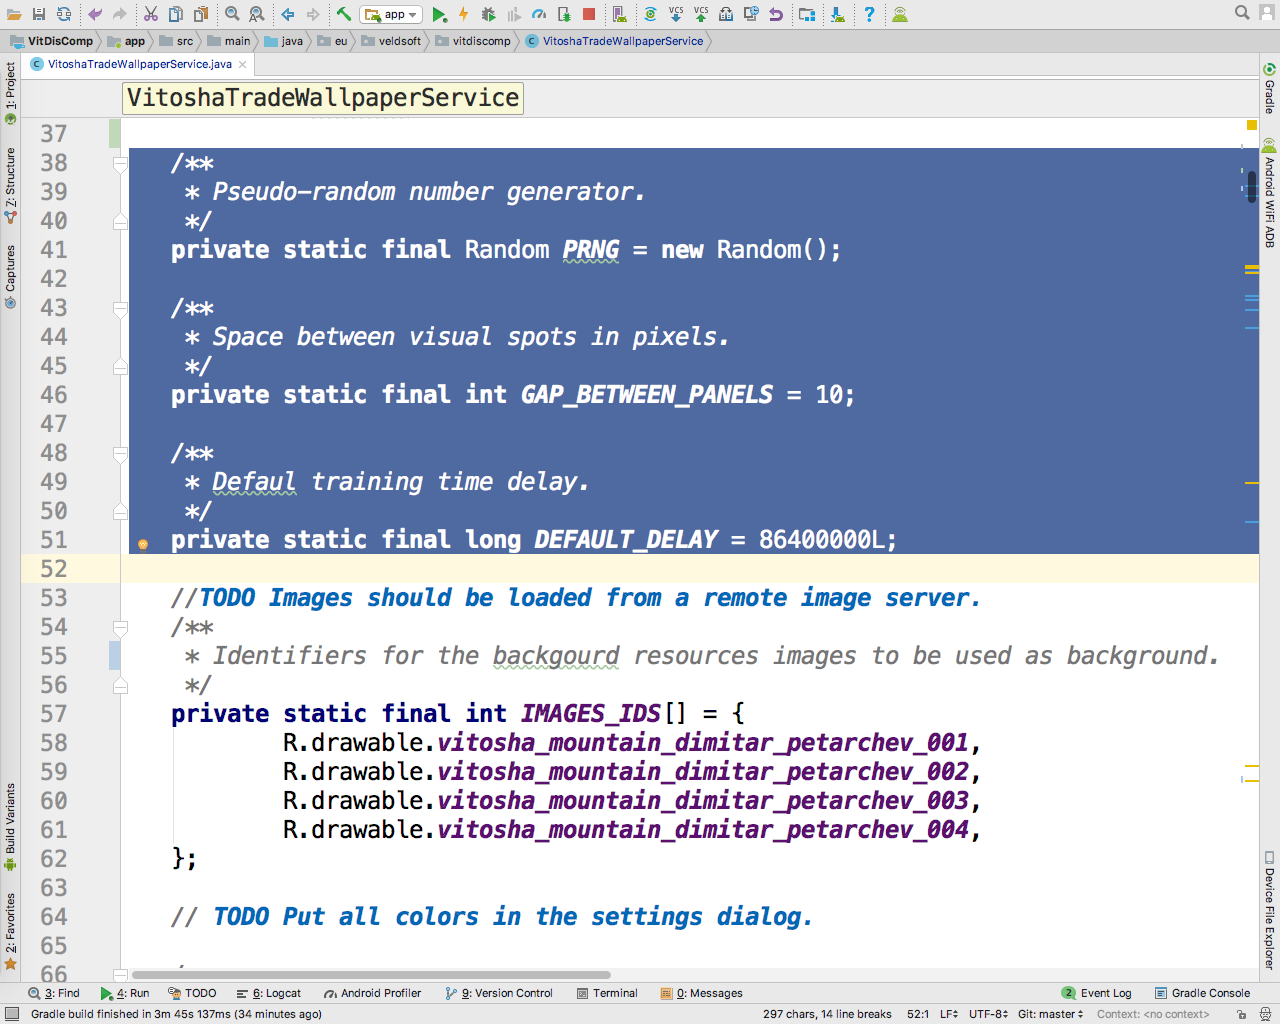
\includegraphics[height=0.45\pdfpageheight]{pic0031}
\caption{Auxiliary constants}
\label{fig:pic0031}
\end{figure}
\FloatBarrier

The colors used for the visual representation are also set with a group of constants but will subsequently be converted to settings with values from the settings window (Fig \ref{fig:pic0032}).

\begin{figure}[h]
\centering
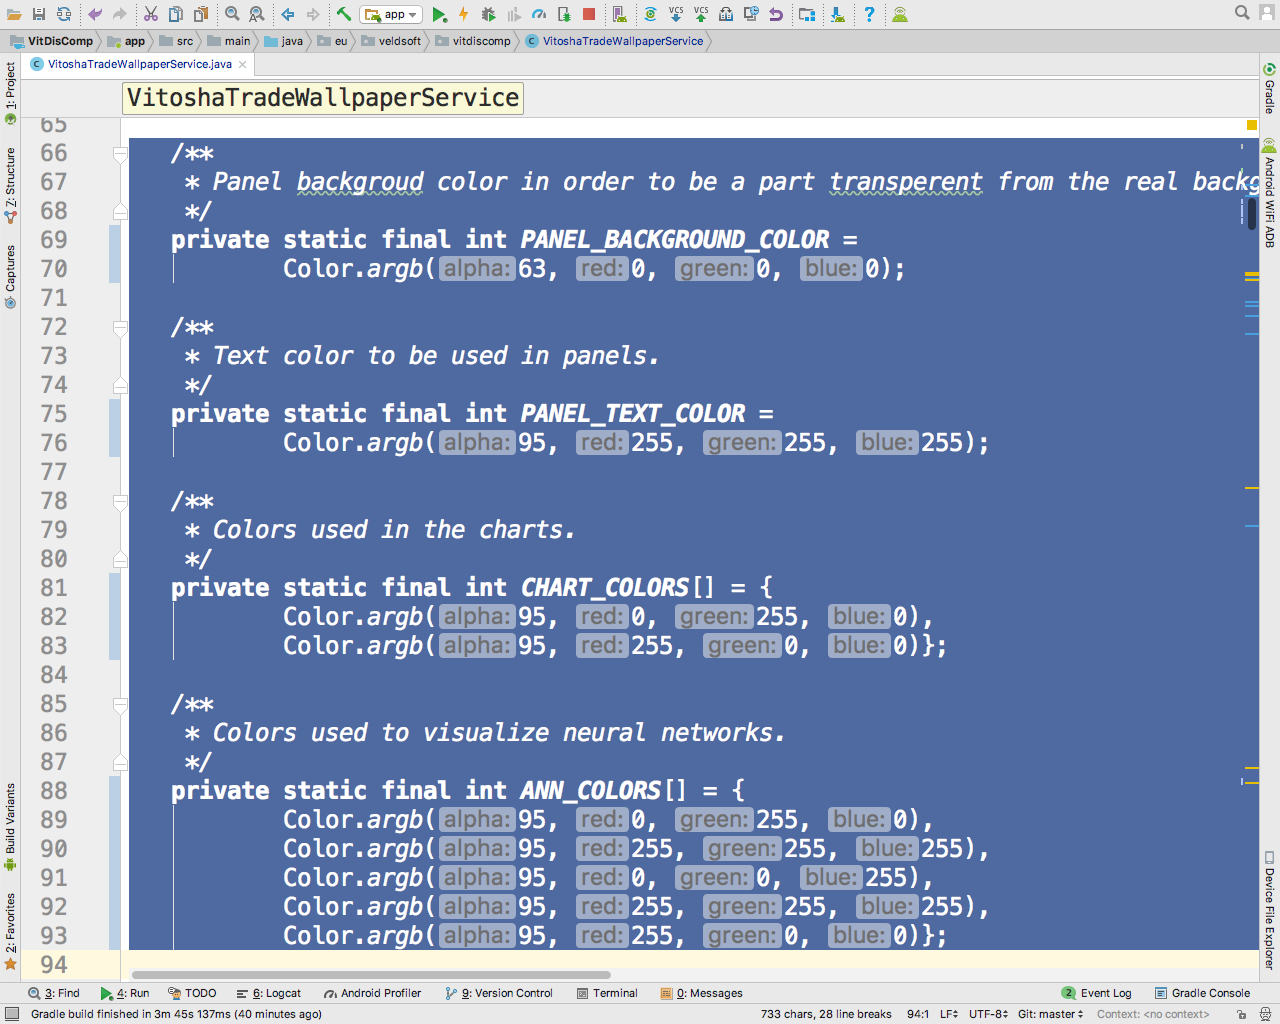
\includegraphics[height=0.45\pdfpageheight]{pic0032}
\caption{Color constants}
\label{fig:pic0032}
\end{figure}
\FloatBarrier

A group of variables is responsible for the state of the active wallpaper. This includes - screen sizes, the time between separate neural network training, whether active wallpaper is on or off, and the exact position of areas for the visual representation of information from the neural network training process (Fig. \ref{fig:pic0033}).

\begin{figure}[h]
\centering
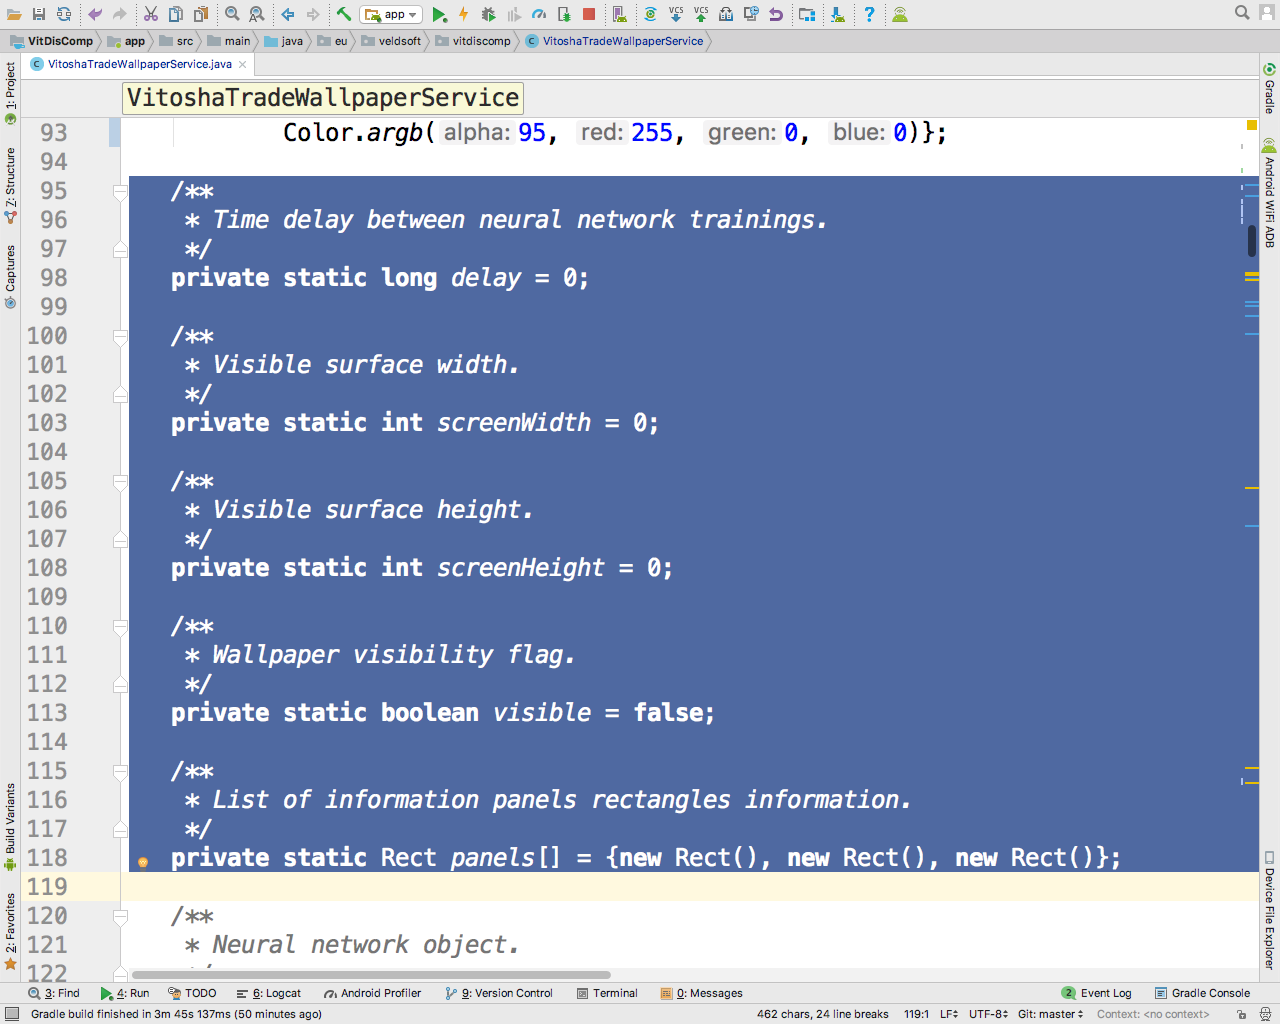
\includegraphics[height=0.45\pdfpageheight]{pic0033}
\caption{Variables reflecting the state of the active wallpaper}
\label{fig:pic0033}
\end{figure}
\FloatBarrier

Another group of variables (references to objects) takes responsibility for managing the artificial neural network, the training examples, the input-output data to the network, and the rule for its training (Fig. \ref{fig:pic0034}).

\begin{figure}[h]
\centering
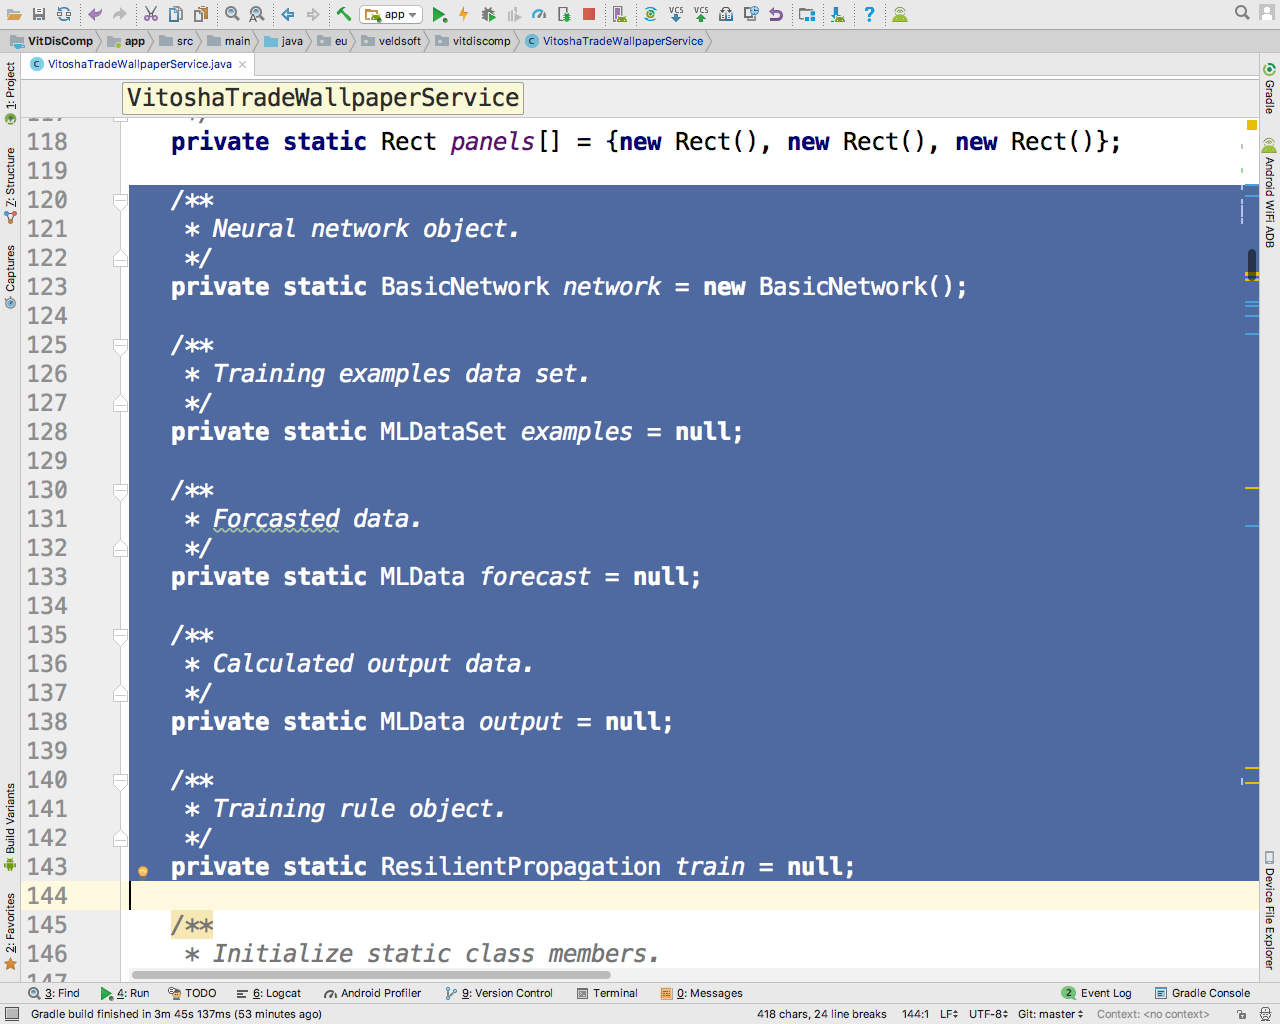
\includegraphics[height=0.45\pdfpageheight]{pic0034}
\caption{Variables responsible for artificial neural network}
\label{fig:pic0034}
\end{figure}
\FloatBarrier

In commercial software production, a widespread trick is to create "software plugs". These are pieces of code that communicate between objects and parts of the system that still need to be made. In the present case, just such a software plug represents the absence of a server and a real data source (Fig. \ref{fig:pic0035}).

\begin{figure}[h]
\centering
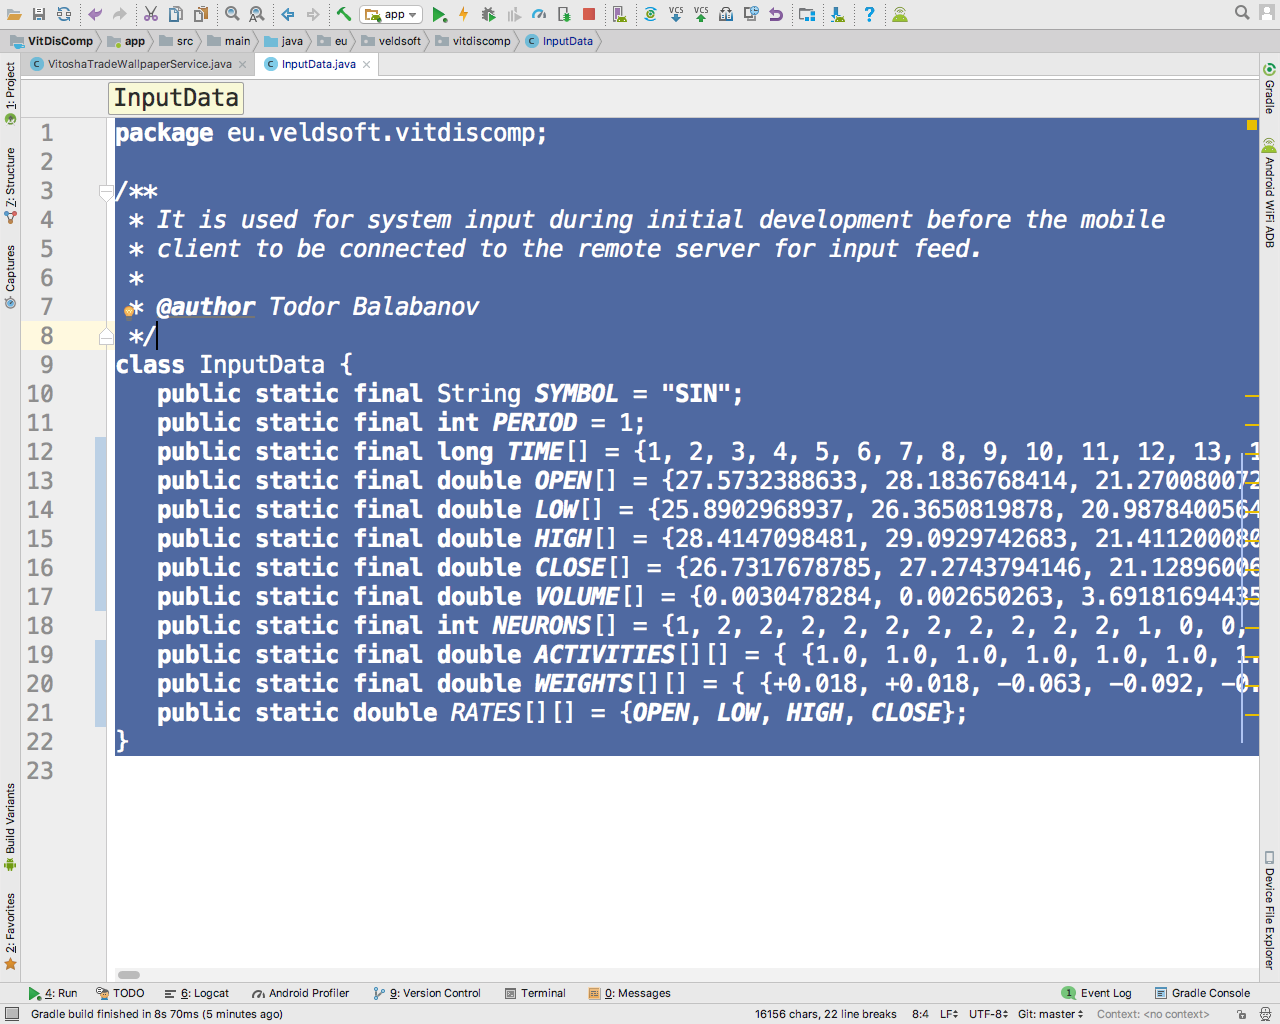
\includegraphics[height=0.45\pdfpageheight]{pic0035}
\caption{Variables responsible for artificial neural network}
\label{fig:pic0035}
\end{figure}
\FloatBarrier

Financial time series are often described with the following characteristics: 1. Type of financial instrument (ticker symbol or stock symbol), in this case, the mathematical function sine; 2. The interval between individual measurements (counted in minutes), in this case, one minute; 3. Six parallel arrays (discrete time, open levels, lowest level reached, the highest level reached, close levels, and volume traded).

In addition to financial information, information about the topology of the artificial neural network must also be submitted to the client application. The description of the artificial neural network requires: 1. Number, arrangement, and type of neurons (a one-dimensional array of constants); 2. Adjacency matrix between neurons (one where there is a connection and zero where there is no connection); 3. The current value of the weight coefficient for each connection between two neurons (including loops, if any).

\begin{figure}[h]
\centering
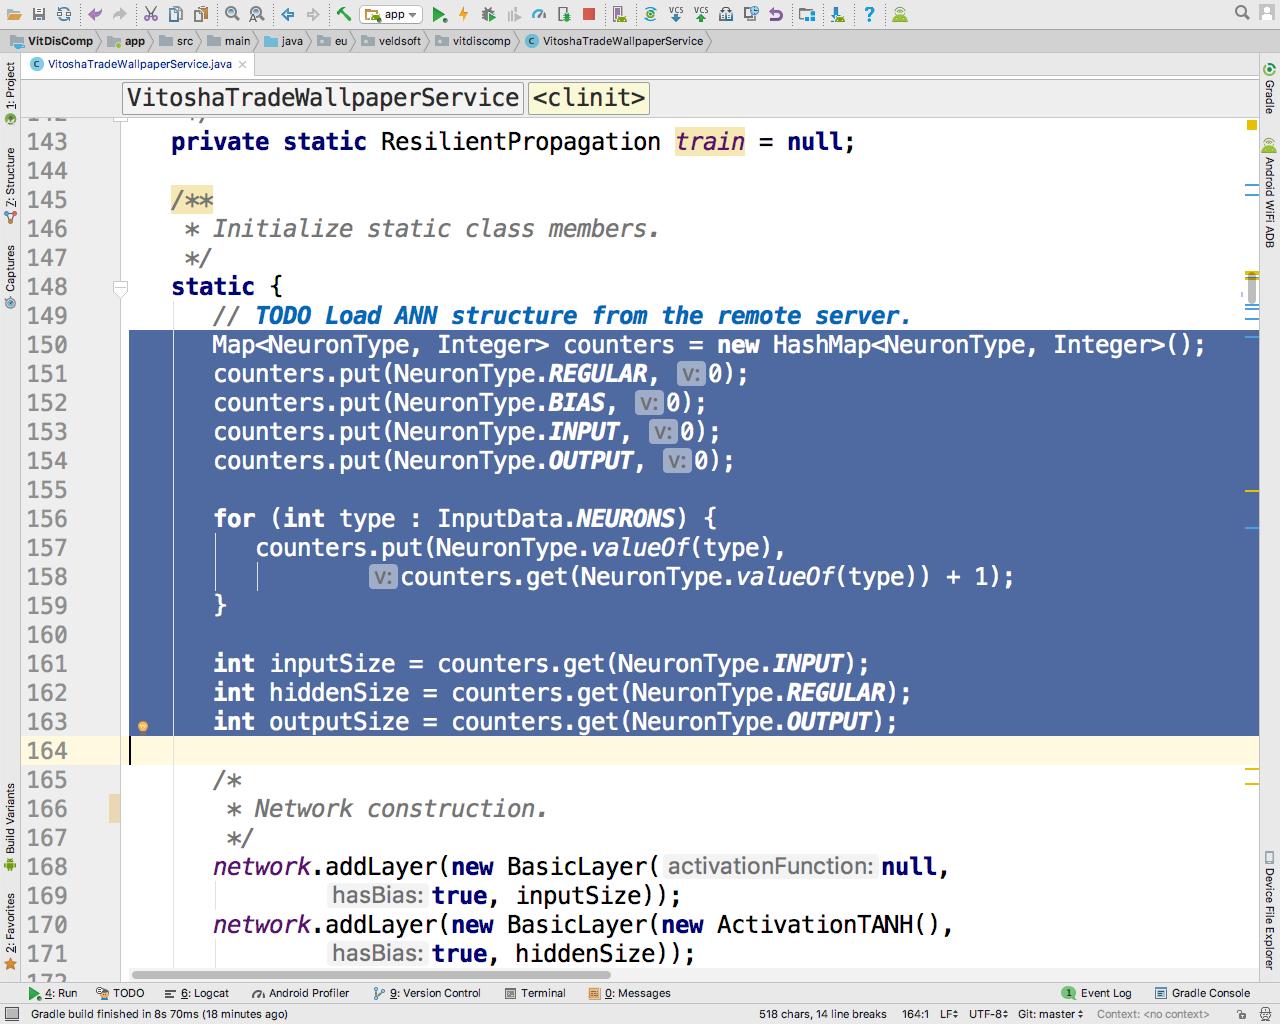
\includegraphics[height=0.45\pdfpageheight]{pic0036}
\caption{Determining the number and types of neurons}
\label{fig:pic0036}
\end{figure}
\FloatBarrier

Counting sorting efficiently determines the number of neurons and their types (Fig. \ref{fig:pic0036}).

\begin{figure}[h]
\centering
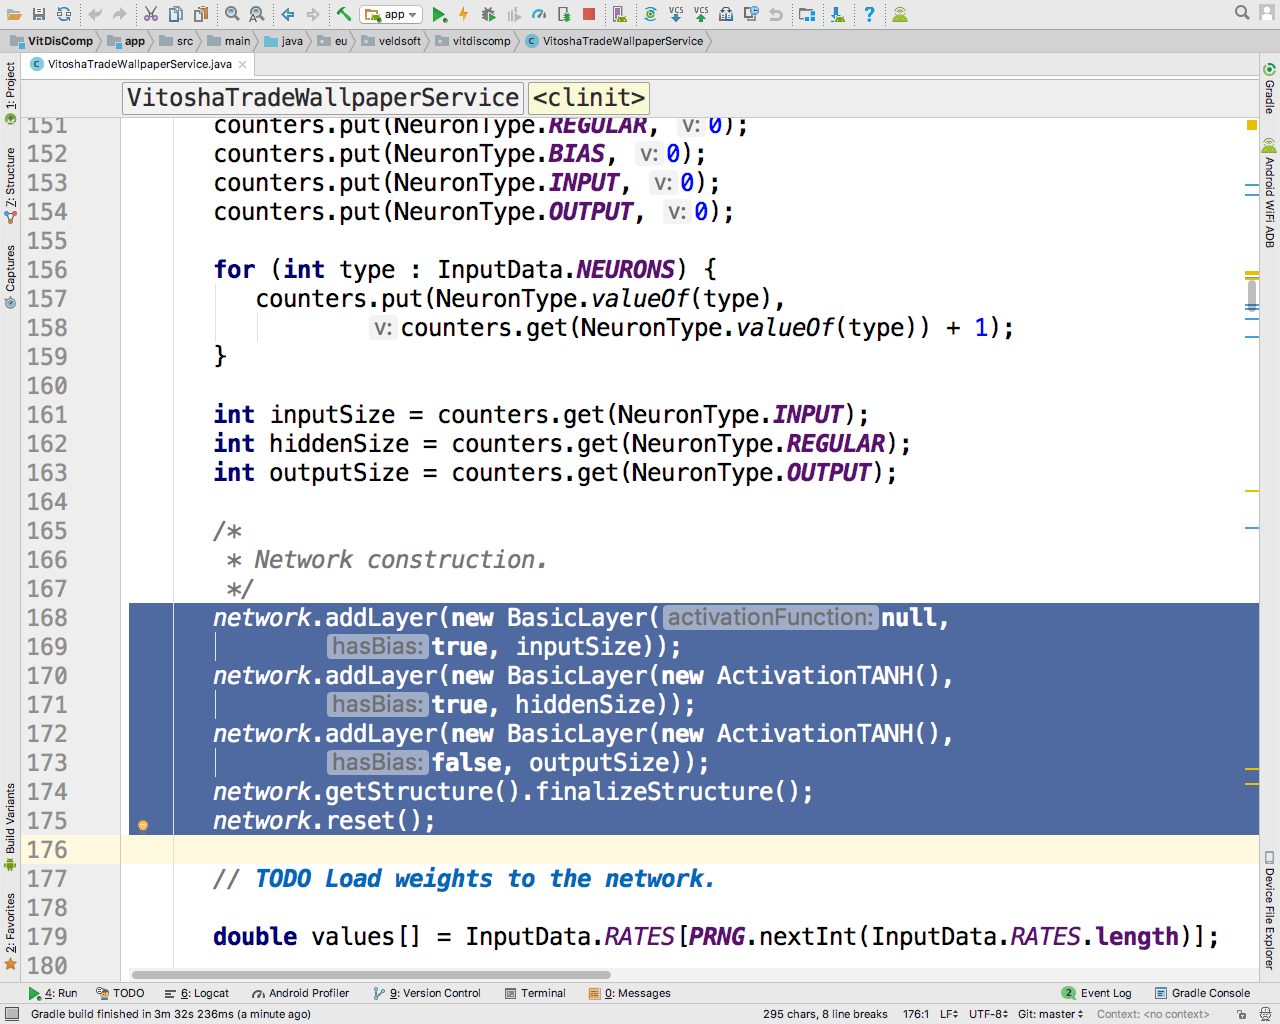
\includegraphics[height=0.45\pdfpageheight]{pic0037}
\caption{Structure of a three-layer artificial neural network}
\label{fig:pic0037}
\end{figure}
\FloatBarrier

To illustrate the predictive capabilities of artificial neural networks, one of the most used topologies is chosen, namely a three-layer neural network that is trained with error backpropagation (Fig. \ref{fig:pic0037}). The input layer has the sole task of receiving the signals from the external environment, so no activation function is set. The function $\tanh( x )$ (hyperbolic tangent) is chosen for the hidden and output layers since it is asymptotically convergent at infinity along the abscissa and, simultaneously, is symmetric along this same axis. Training is slightly faster with a hyperbolic tangent because the signal values in the hidden layers are more easily "skewed" in a positive or negative direction. In comparison, with the sigmoid function, the signals are only positive; if negative values are needed, this compensation must be obtained only through negative link weights. The input and hidden layers have a bias neuron that is not required in the output layer because the bias neuron constantly emits the high-level signal.

\begin{figure}[h]
\centering
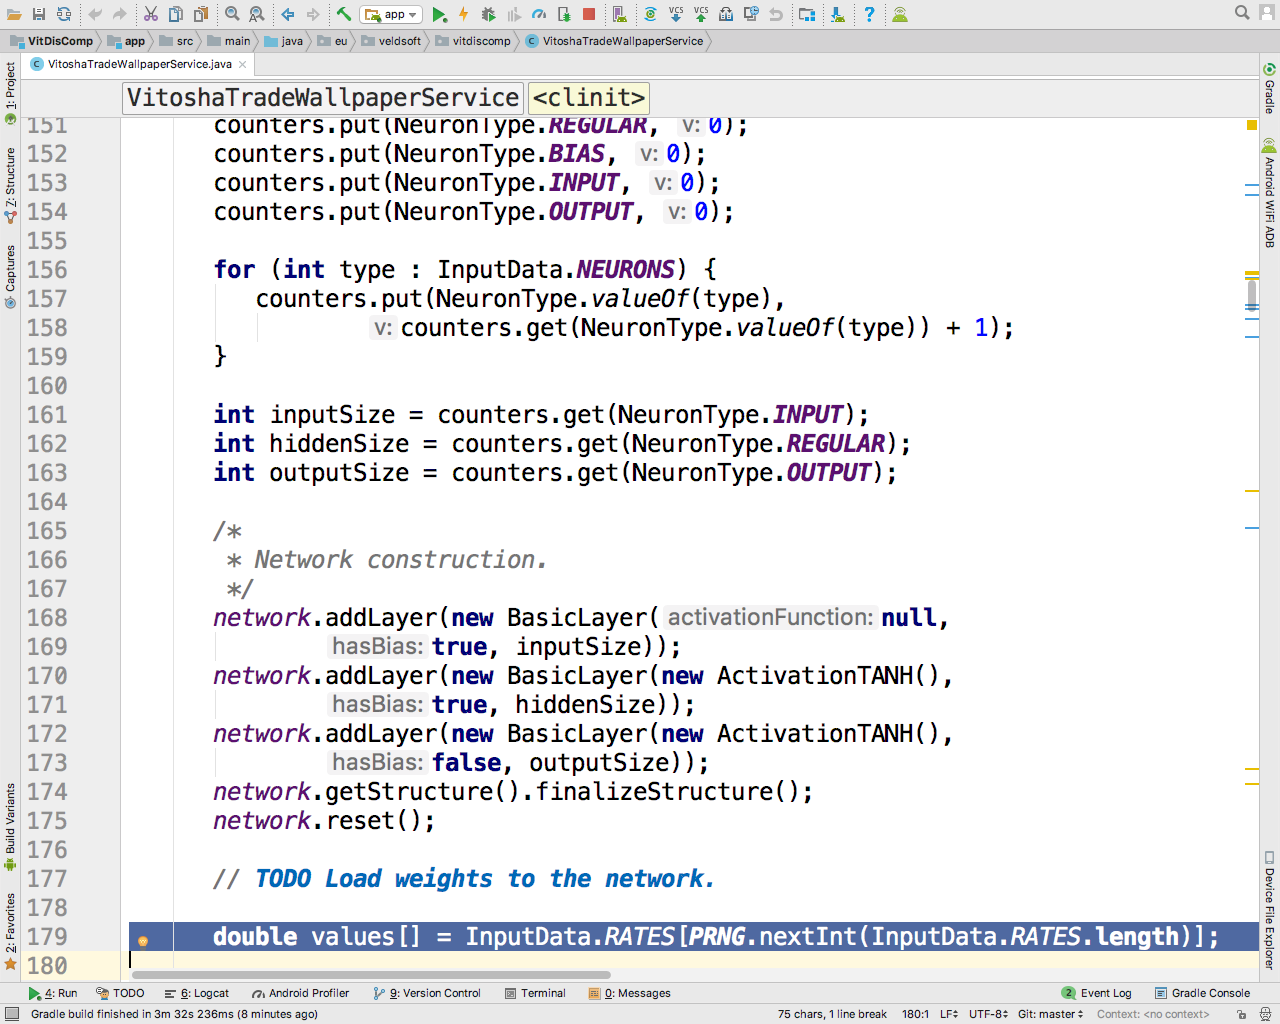
\includegraphics[height=0.45\pdfpageheight]{pic0038}
\caption{Choosing values to predict}
\label{fig:pic0038}
\end{figure}
\FloatBarrier

From the description of parallel arrays in financial time series, it is clear that there are four possible sequences of numbers to feed to the neural network for prediction (open, low, high, and close).

\begin{figure}[h]
\centering
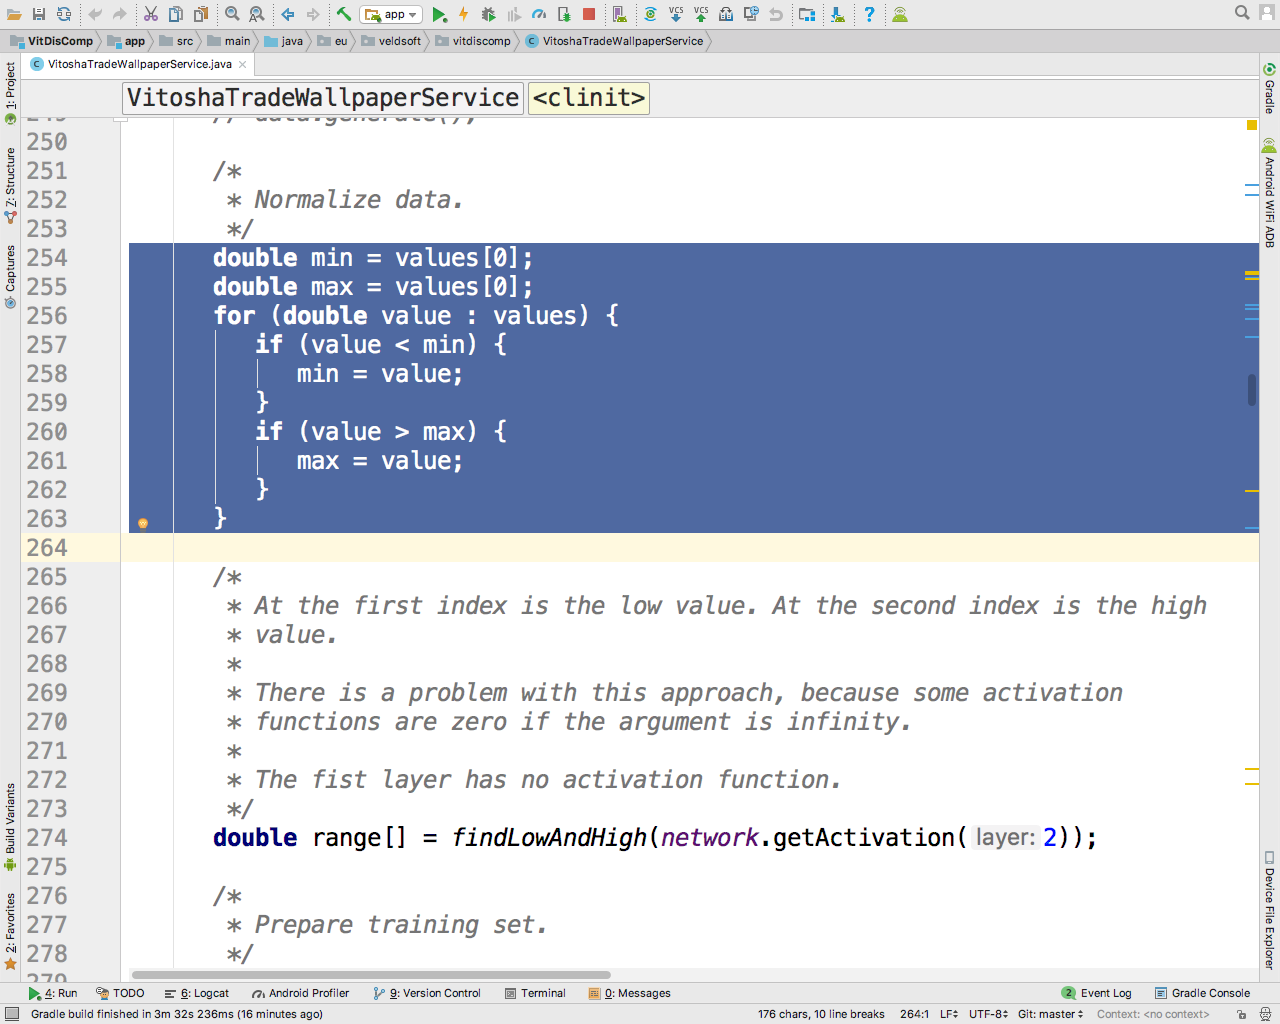
\includegraphics[height=0.45\pdfpageheight]{pic0039}
\caption{Determining boundaries in the time series}
\label{fig:pic0039}
\end{figure}
\FloatBarrier

In practice, the closing value series is most often used, and the purpose is to predict the opening level in the next time interval. The objectives of this presentation are not to achieve financial predictions, and for this reason, it is a randomly chosen sequence to use in the different training/forecasting runs (Fig. \ref{fig:pic0038}).

\begin{figure}[h]
\centering
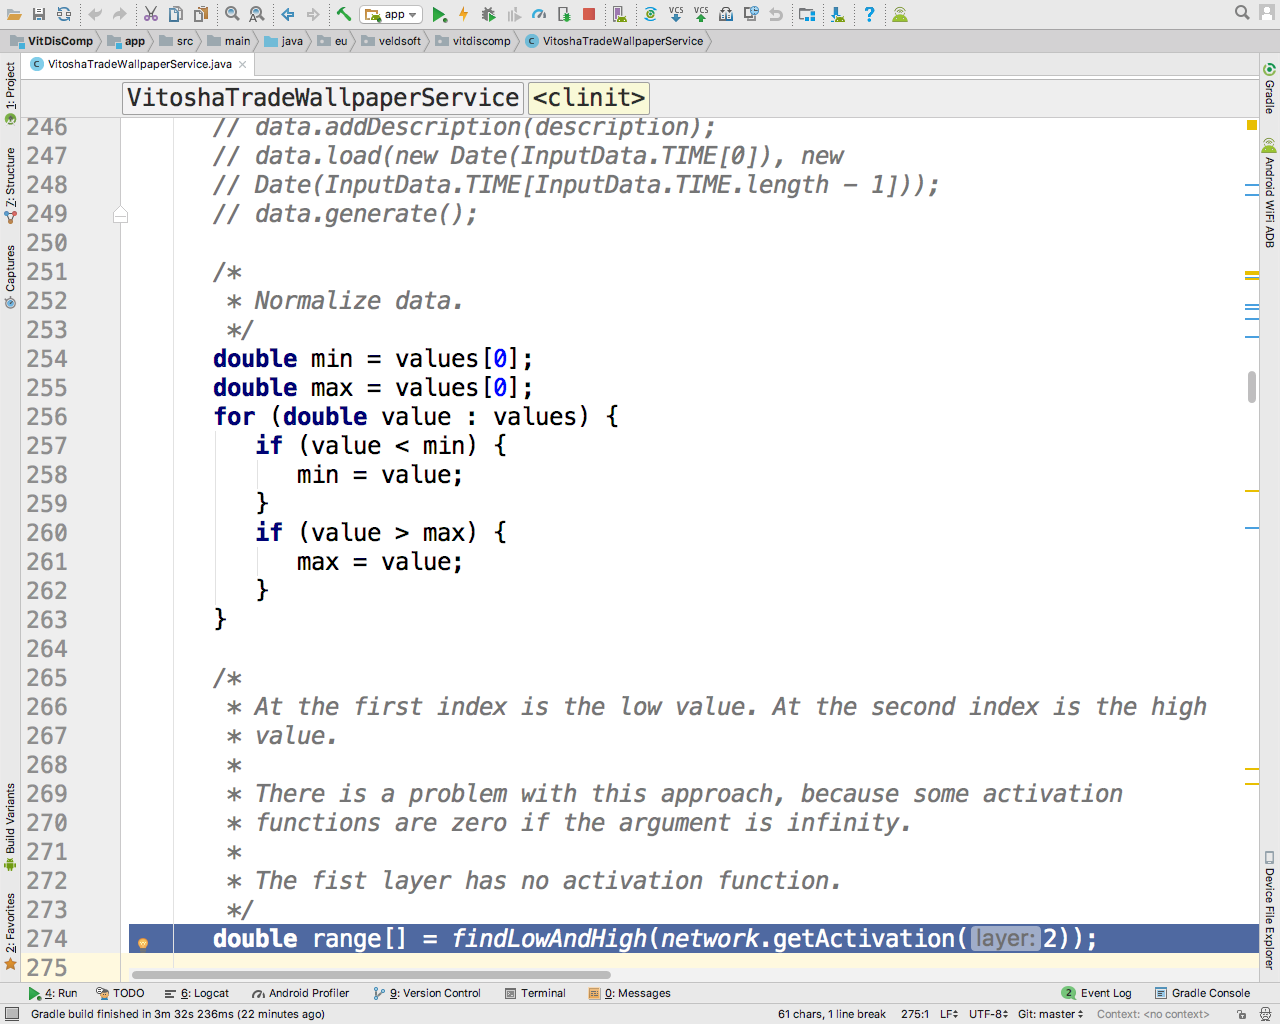
\includegraphics[height=0.45\pdfpageheight]{pic0040}
\caption{Range of the activation function in the output layer}
\label{fig:pic0040}
\end{figure}
\FloatBarrier

Since the goal is to feed different financial time series to the forecasting system, the input information in the system inevitably needs to be pre-normalized, and the first step to this is to determine the most significant and most minor values in the time series ( Fig. \ref{fig:pic0039}). At the same time, the data must be matched to the range in which the activation functions of the artificial neural network work. This tutorial assumes that signals in the scope of the function used in the output layer will be applied to the input (Fig. \ref{fig:pic0040}). This decision is explained by the fact that the information fed by the neural network to the external environment will undergo a reverse resizing process to make sense of the particular financial time series.

\begin{figure}[h]
\centering
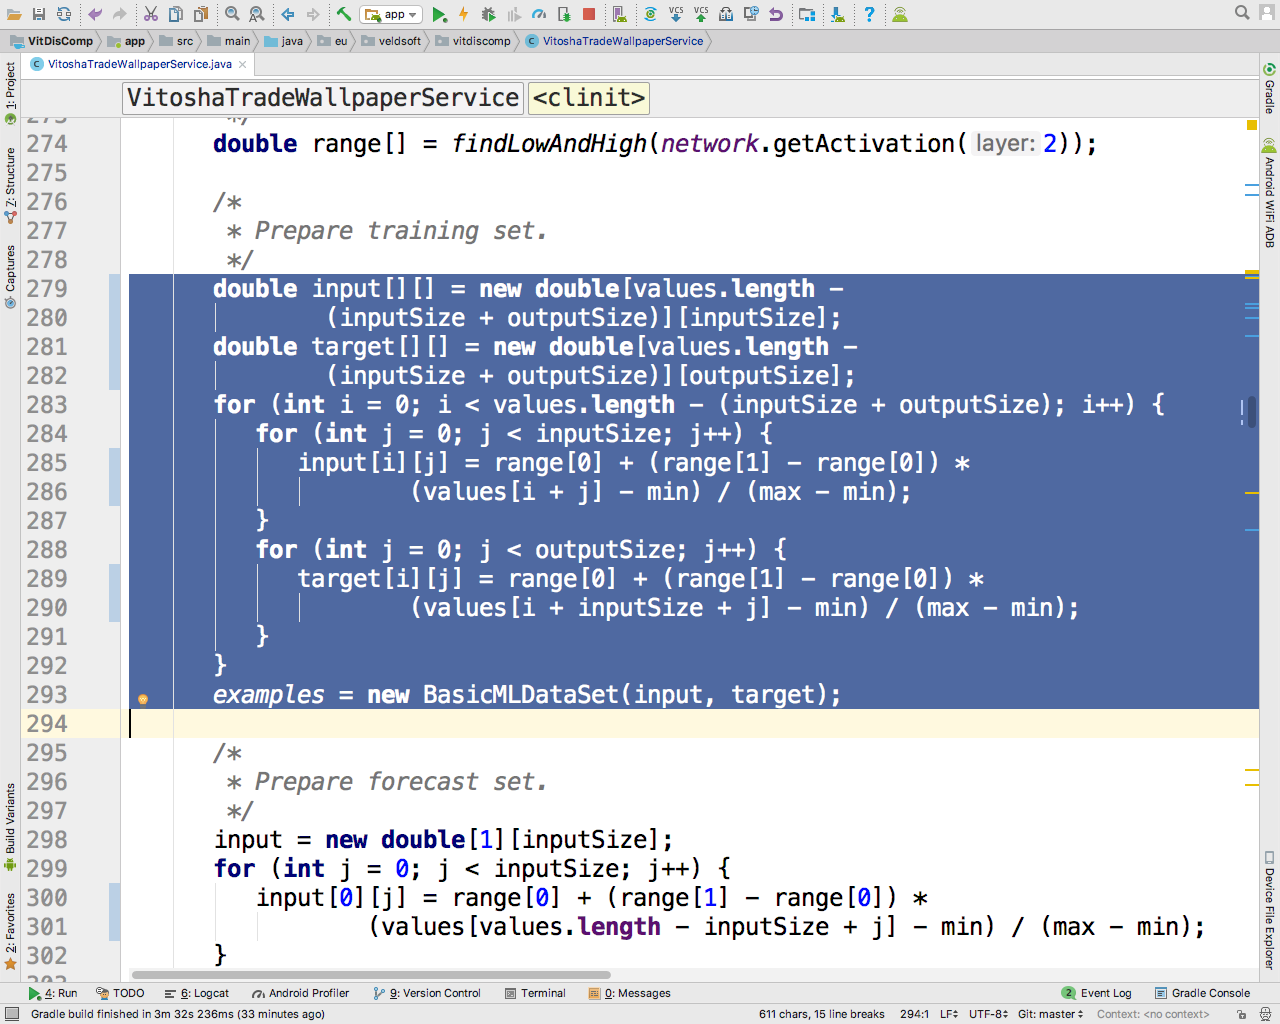
\includegraphics[height=0.45\pdfpageheight]{pic0041}
\caption{Training examples}
\label{fig:pic0041}
\end{figure}
\FloatBarrier

We conditionally divide the normalized input data into two sets (measurements in the past and measures in the future). The separation is conditional since practically the data are from real measurements in the past (Fig. \ref{fig:pic0041}).

\begin{figure}[h]
\centering
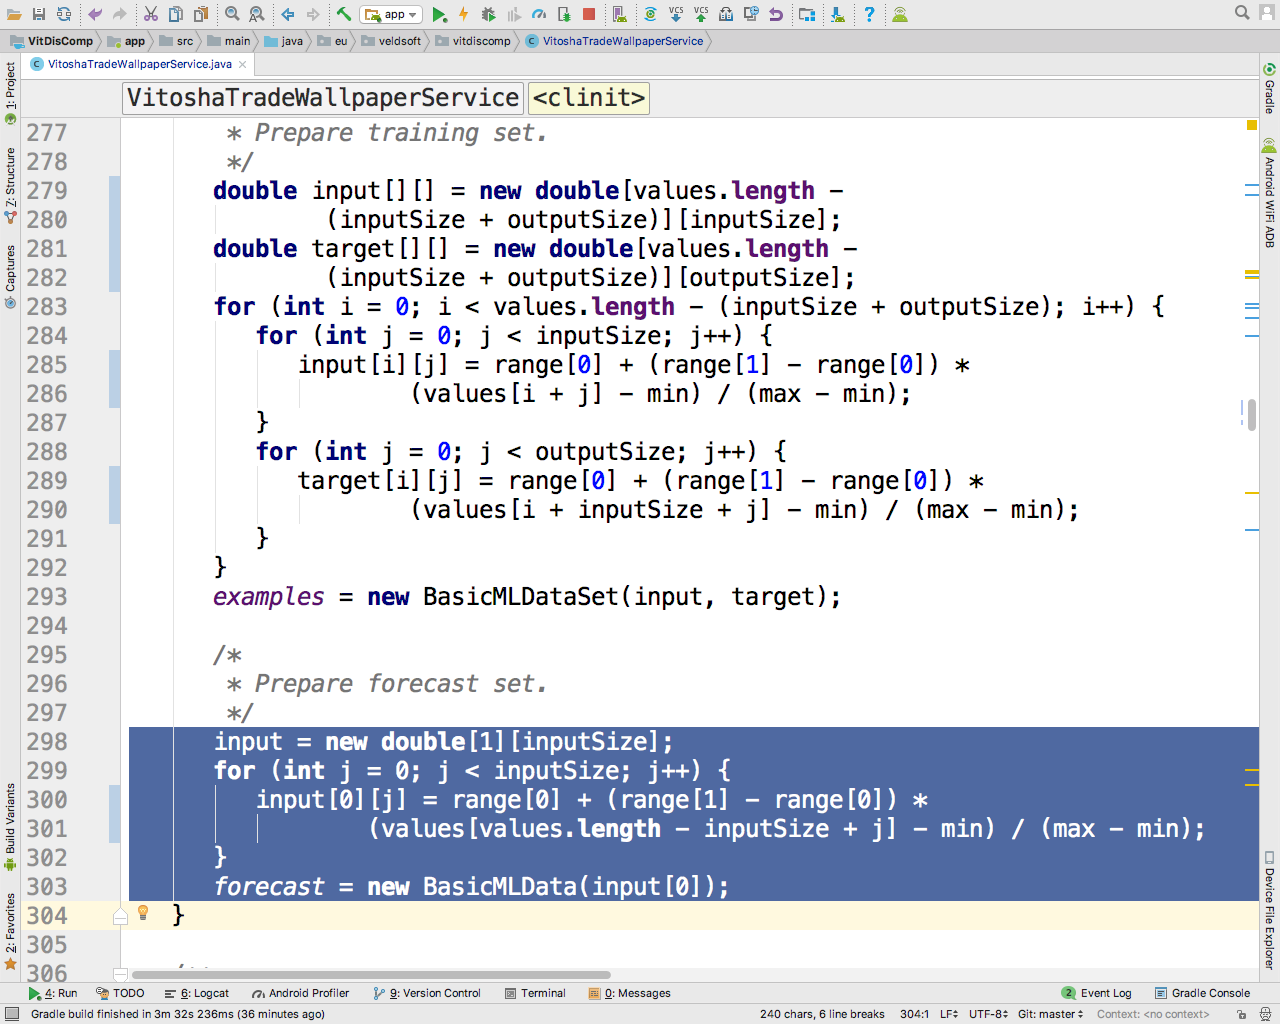
\includegraphics[height=0.45\pdfpageheight]{pic0042}
\caption{Input to the artificial neural network to obtain a prediction}
\label{fig:pic0042}
\end{figure}
\FloatBarrier

Since the artificial neural network is used in both its modes (training and prediction), it also prepares a vector of input data against which to make a prediction (Fig. \ref{fig:pic0042}).

\begin{figure}[h]
\centering
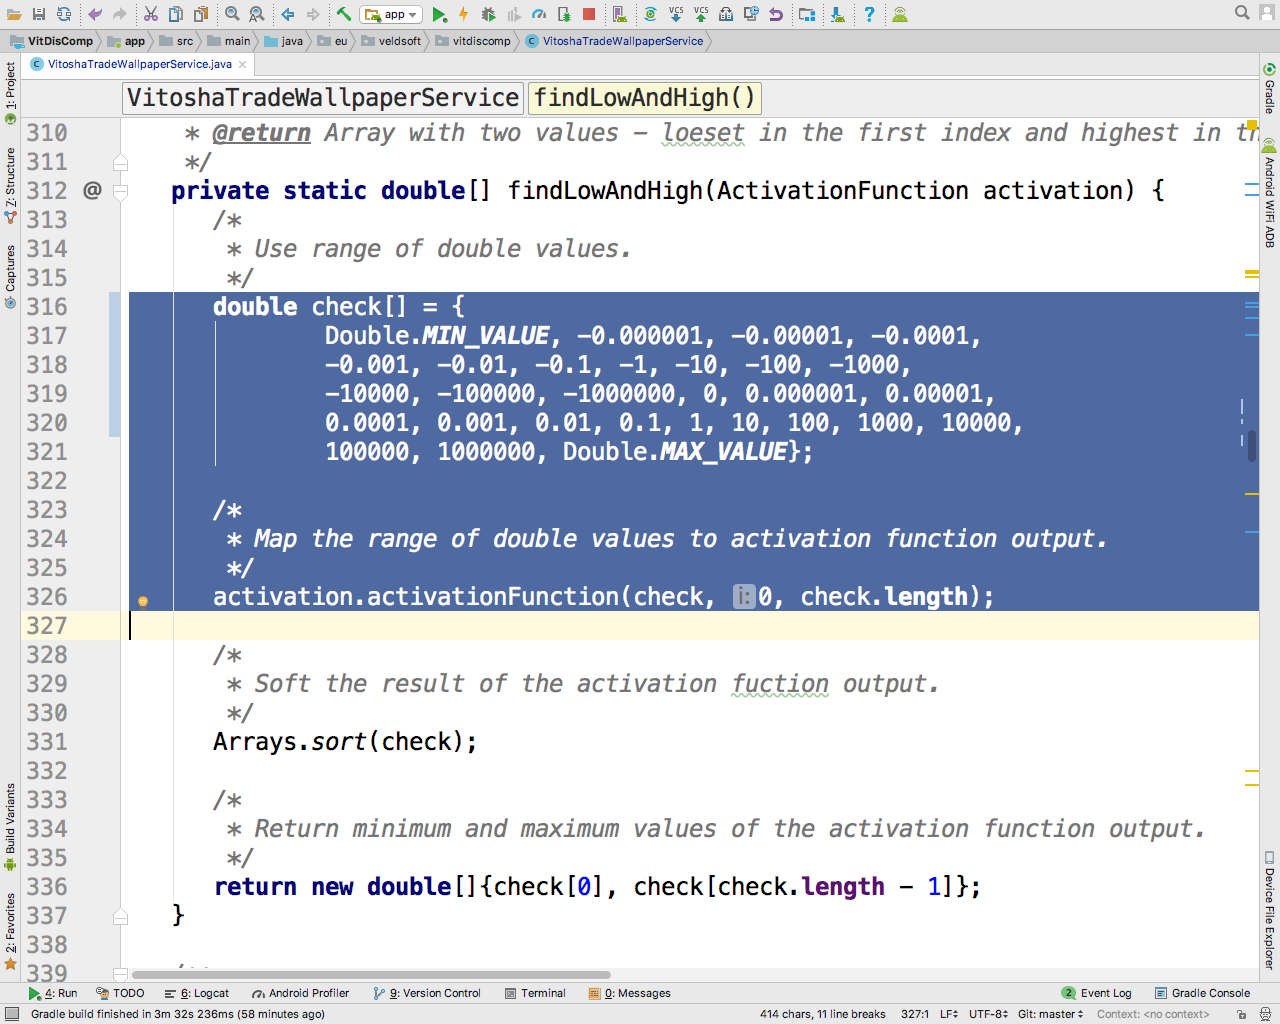
\includegraphics[height=0.45\pdfpageheight]{pic0043}
\caption{Exploring a group of values to determine the range}
\label{fig:pic0043}
\end{figure}
\FloatBarrier

In general, the activation functions have asymptotic convergence and are monotonically increasing (Fig. \ref{fig:pic0044}), which allows their finite ranges to be established by inspecting a set of values (Fig. \ref{fig:pic0043}).

\begin{figure}[h]
\centering
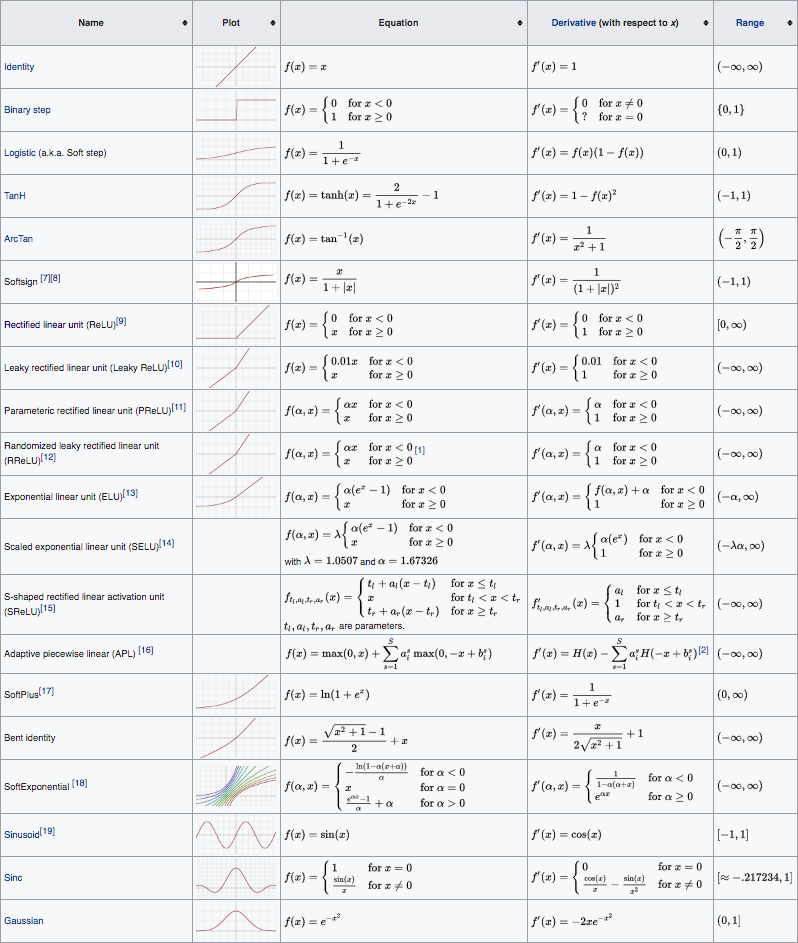
\includegraphics[height=0.7\pdfpageheight]{pic0044}
\caption{Activation Functions \cite{afwiki}}
\label{fig:pic0044}
\end{figure}
\FloatBarrier

As is visible in Fig. \ref{fig:pic0044}, for some of the activation functions, such a range determination can be highly misleading (e.g., the sine function).

\begin{figure}[h]
\centering
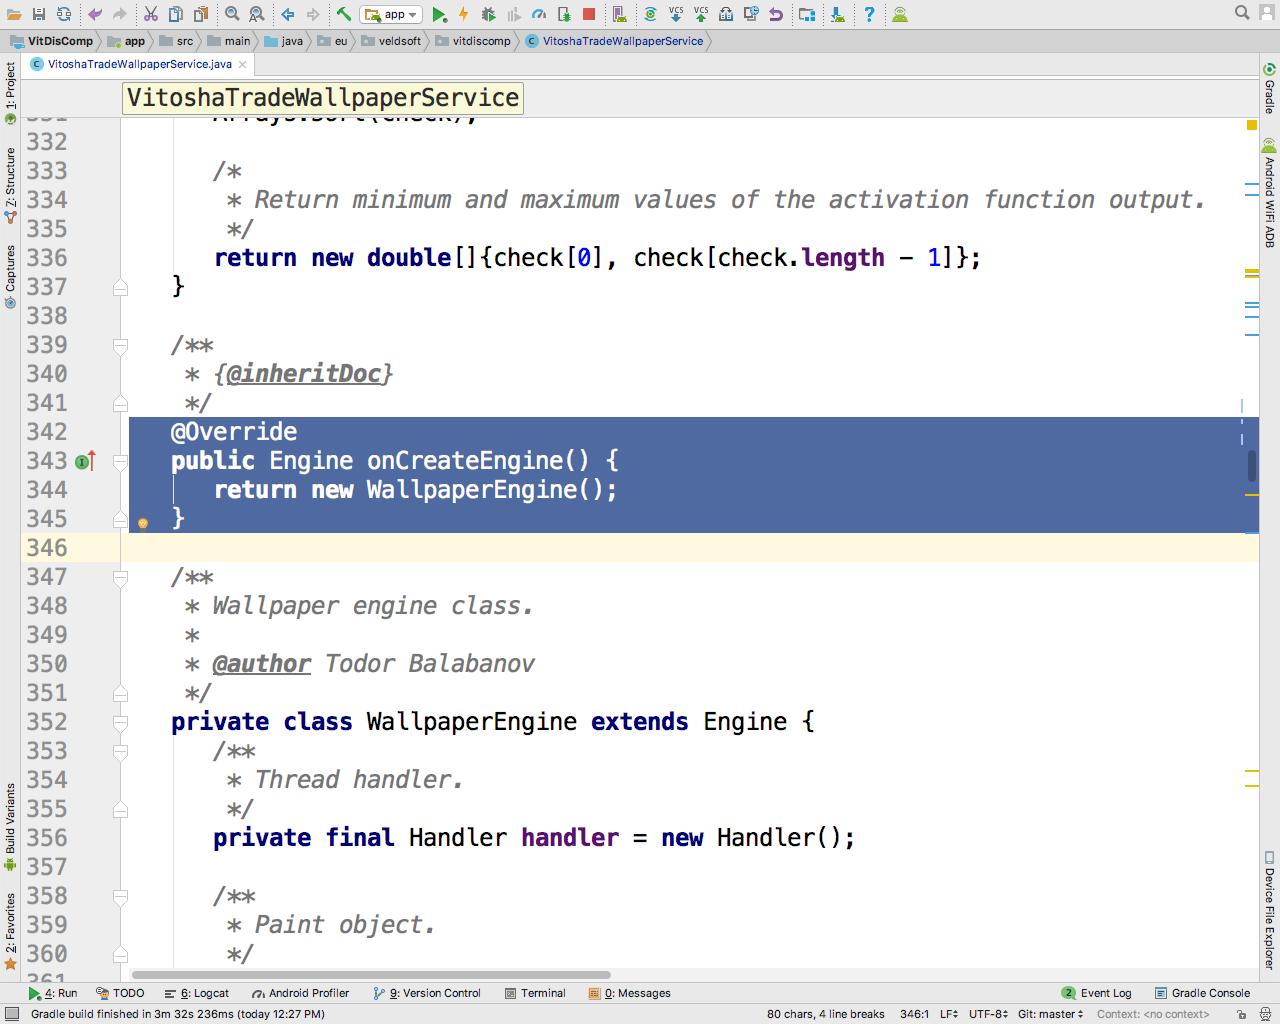
\includegraphics[height=0.45\pdfpageheight]{pic0045}
\caption{Custom implementation of the inherited Engine class and object creation}
\label{fig:pic0045}
\end{figure}
\FloatBarrier

The engine object creation event is redefined to return an object from our engine class (Fig \ref{fig:pic0045}).

\section{Service Engine}

The actual background computation work in the service is done by an object described by a private inner class of type "Engine".

\begin{figure}[h]
\centering
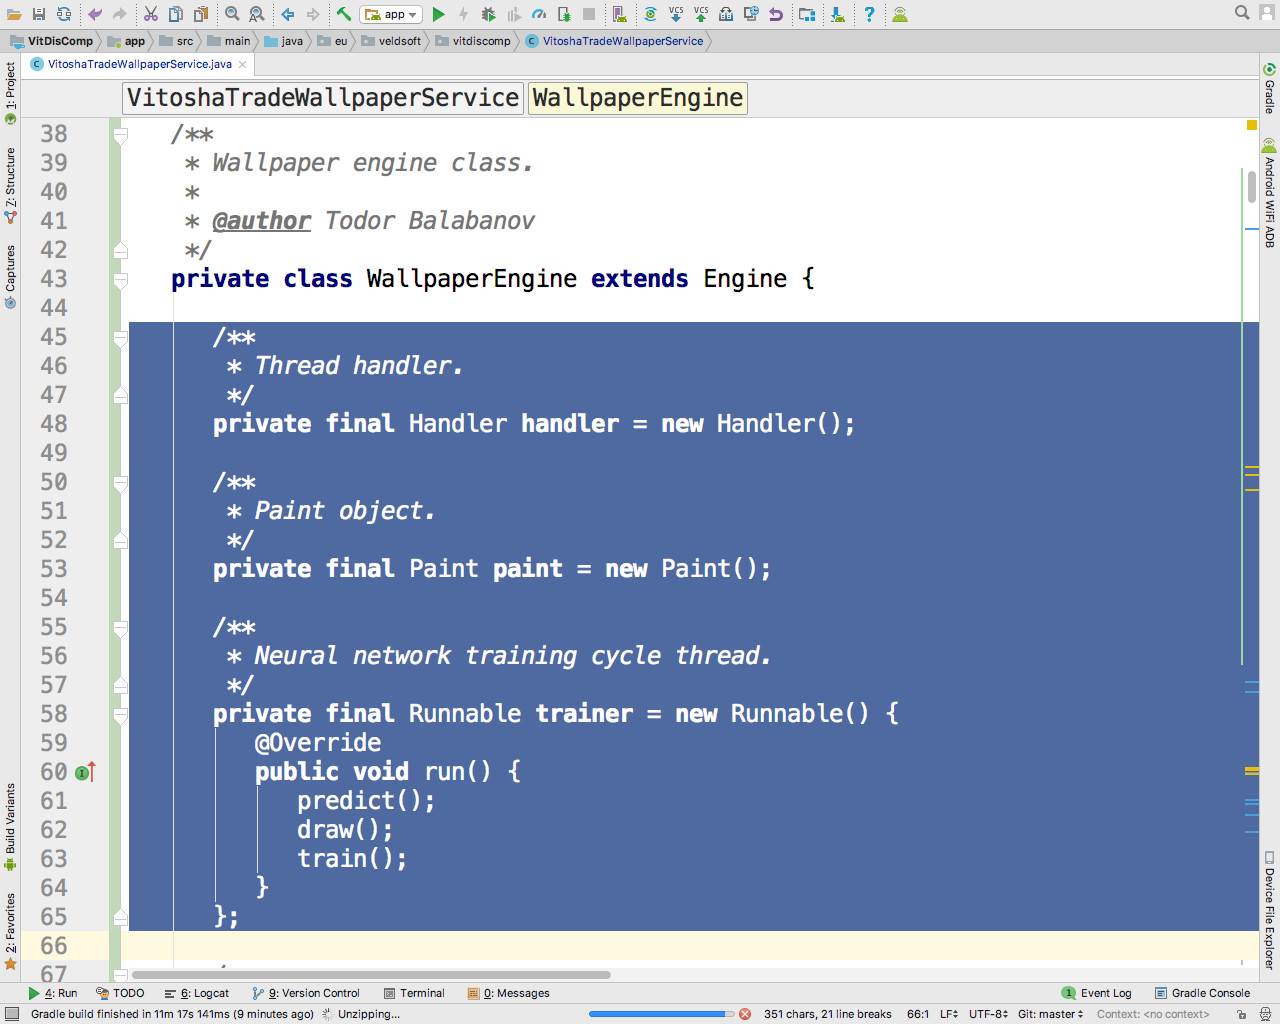
\includegraphics[height=0.45\pdfpageheight]{pic0046}
\caption{Internal variables for the service engine}
\label{fig:pic0046}
\end{figure}
\FloatBarrier

Three internal variables are used in this engine (Fig \ref{fig:pic0046}). The object of type "brush" (Paint) is only auxiliary and serves to define the characteristics of painting once. The benefit is that the object is created once and then used throughout the service's life cycle.

\begin{figure}[h]
\centering
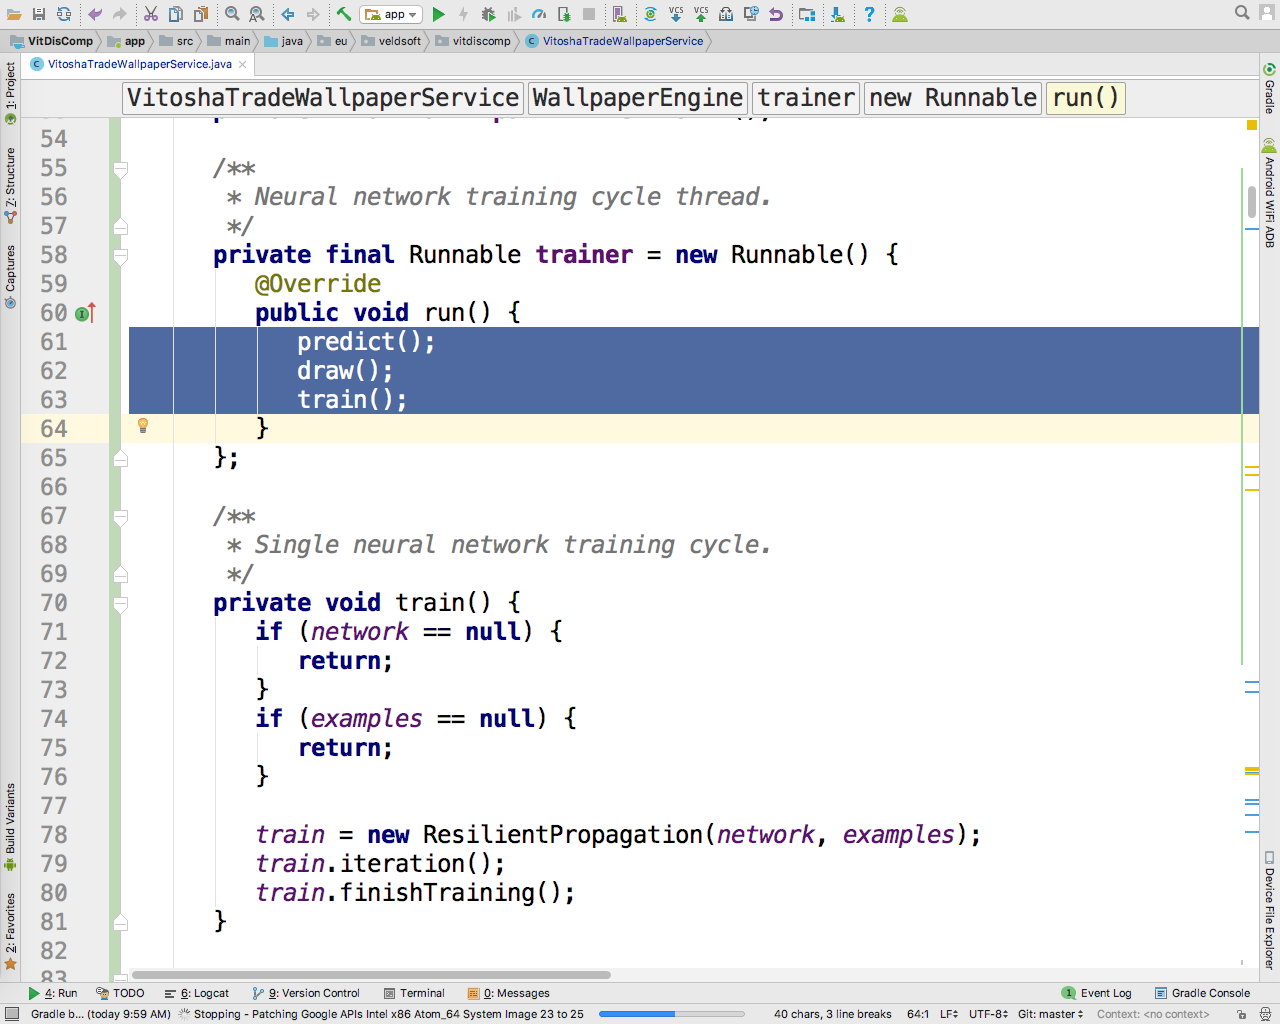
\includegraphics[height=0.45\pdfpageheight]{pic0047}
\caption{Single loop in background}
\label{fig:pic0047}
\end{figure}
\FloatBarrier

For the actual operation of the engine, a separate thread (trainer) is defined to perform the operations of generating a prediction, drawing the active wallpaper, and completing one cycle of the training process of the artificial neural network\index{artificial neural networks} (Fig. \ref {fig:pic0047}). Effective thread management in Android is done using Handler objects. The Handler object takes responsibility for starting the thread, stopping the thread, and implementing the timeout interval before the next wakeup of the thread occurs.

\begin{figure}[h]
\centering
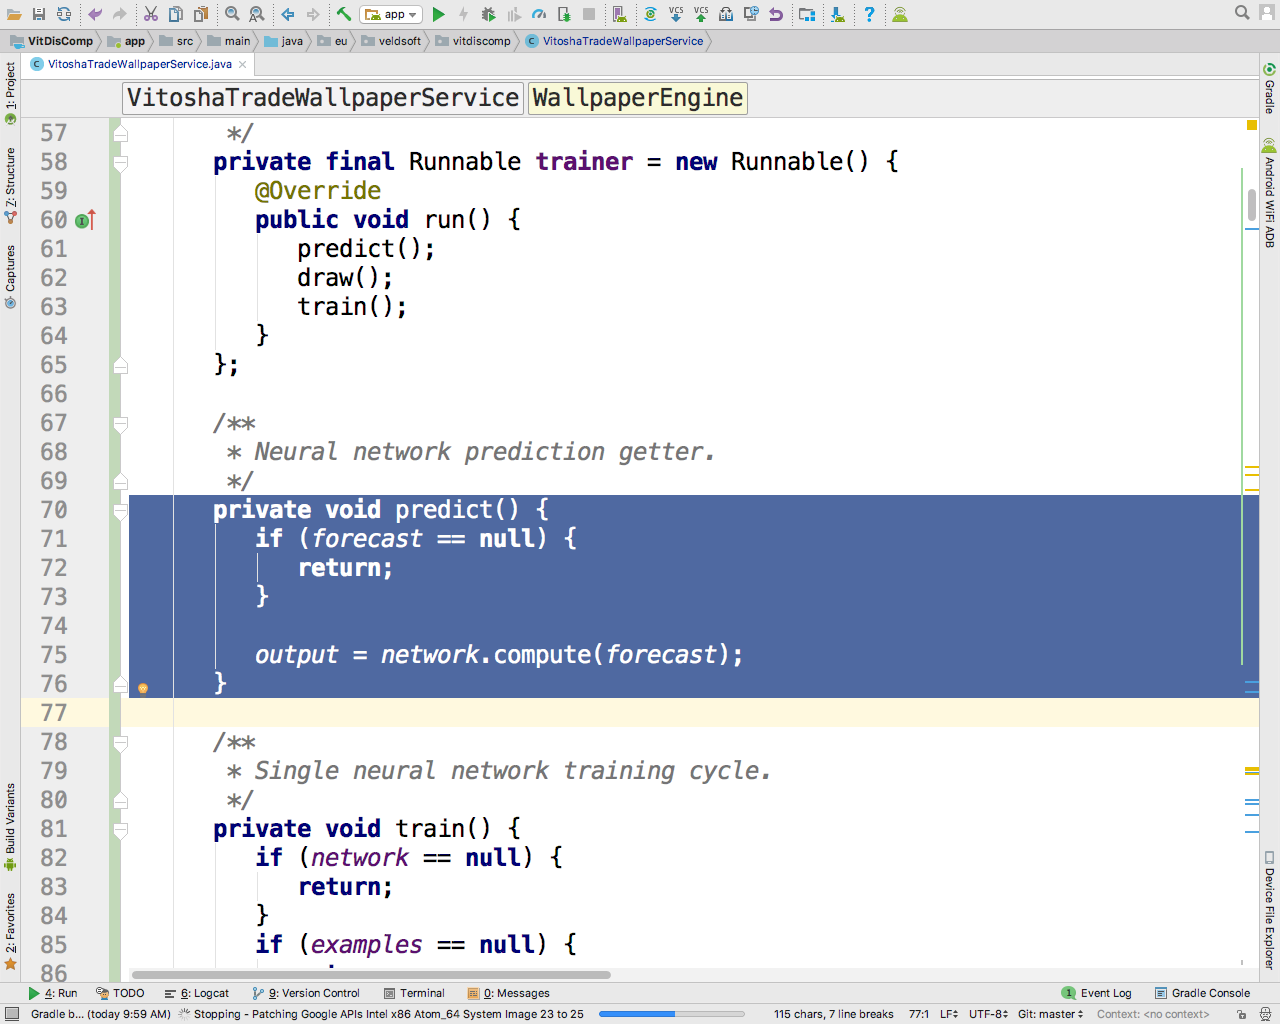
\includegraphics[height=0.45\pdfpageheight]{pic0048}
\caption{Prediction calculation}
\label{fig:pic0048}
\end{figure}
\FloatBarrier

To calculate a prediction, according to the current level of training of the artificial neural network\index{artificial neural networks}, it is enough to activate the network in working mode with appropriate data to the input layer (Fig. \ref{fig:pic0048}).

\begin{figure}[h]
\centering
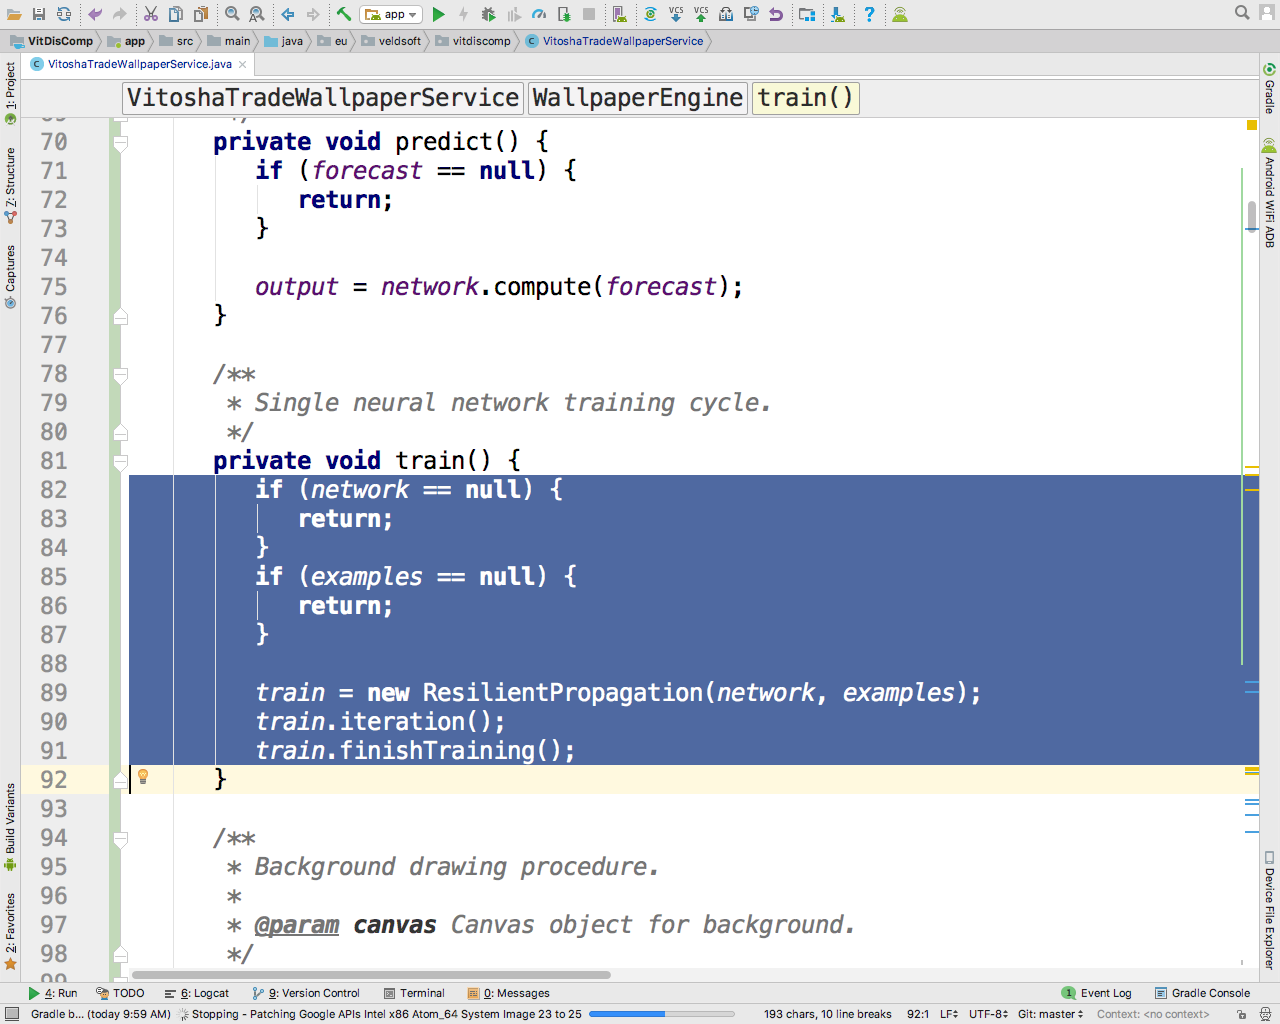
\includegraphics[height=0.45\pdfpageheight]{pic0049}
\caption{Training cycle of the artificial neural network}
\label{fig:pic0049}
\end{figure}
\FloatBarrier

To perform one training cycle of the artificial neural network\index{artificial neural networks}, it is enough to create a training object (in the case of elastic backpropagation of the error\index{backpropagation of the error}) to which the network and training examples are fed (Fig. \ref{fig:pic0049}).

\begin{figure}[h]
\centering
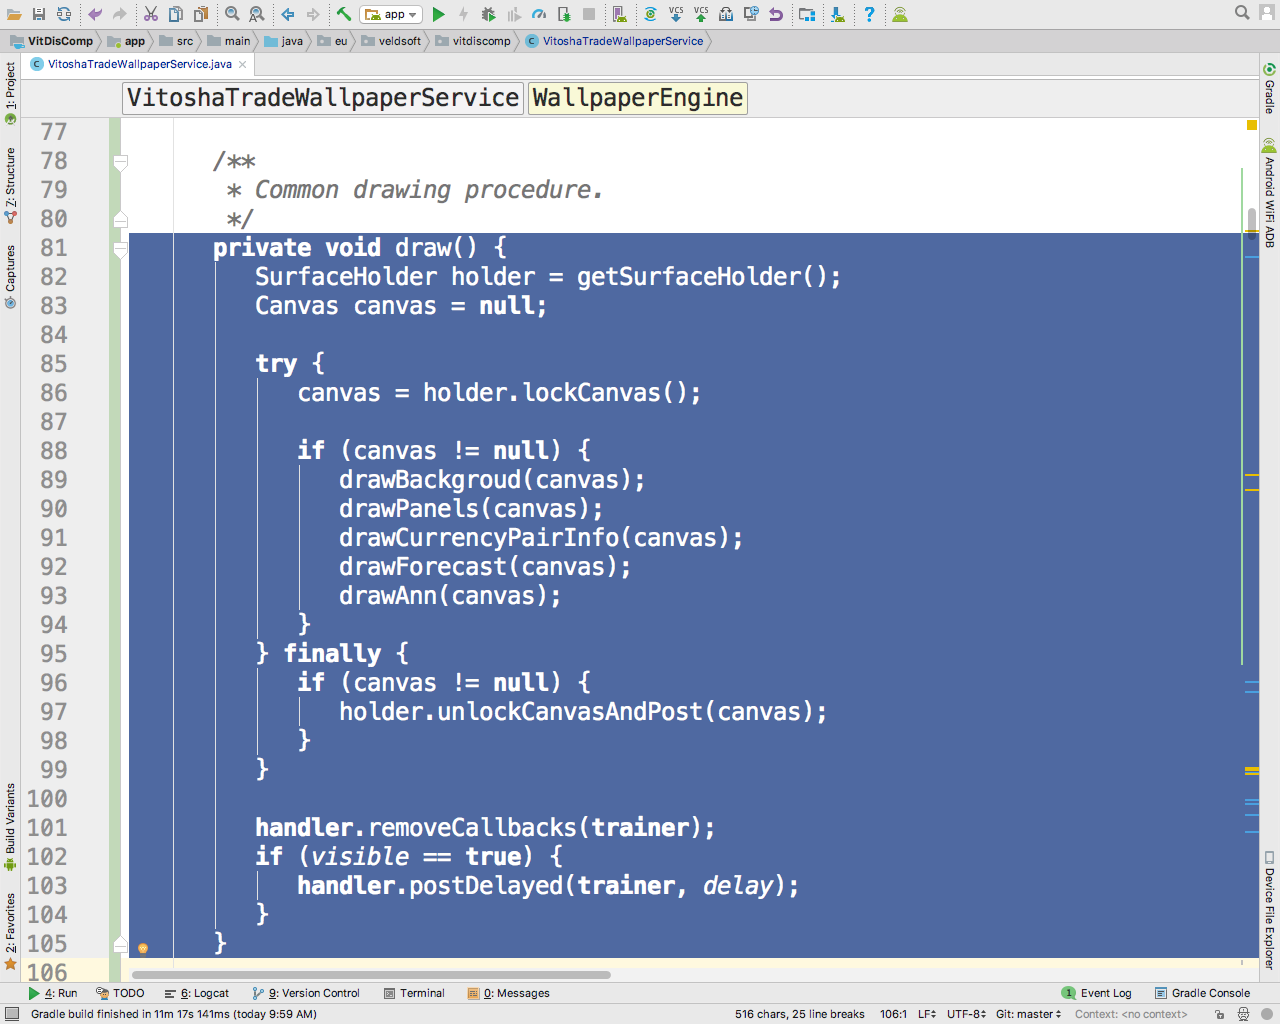
\includegraphics[height=0.45\pdfpageheight]{pic0050}
\caption{Basic procedure for plotting the information from the training process}
\label{fig:pic0050}
\end{figure}
\FloatBarrier

Drawing the information from the training process is organized in a separate function (Fig. \ref{fig:pic0050}). For the visual representation to take place, access is provided to the surface and the canvas it contains. At the very end of the visualization function, a decision is made whether to execute the next training cycle or abort execution.

\begin{figure}[h]
\centering
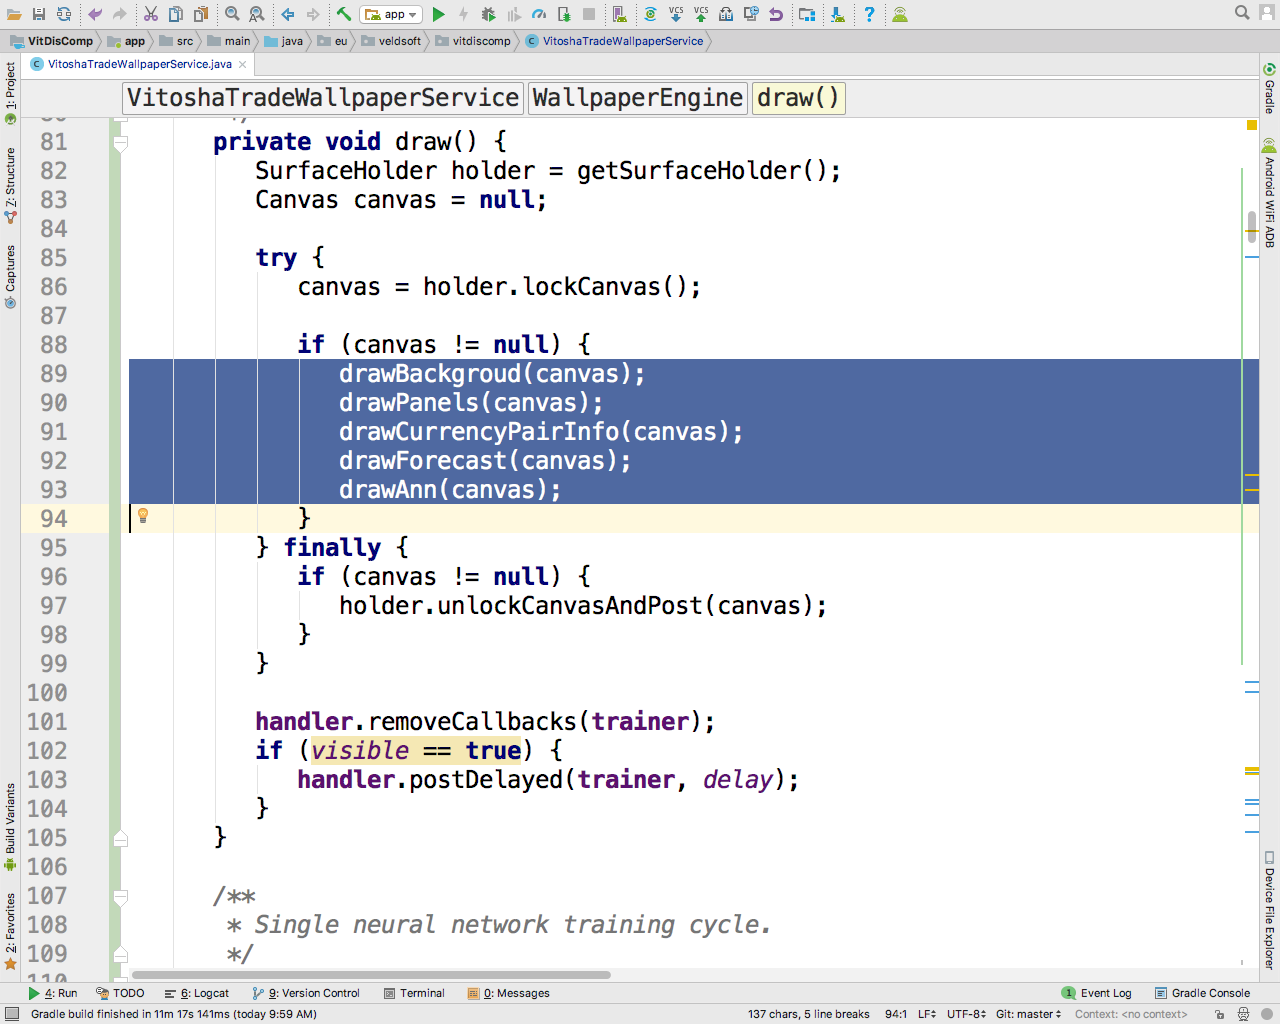
\includegraphics[height=0.45\pdfpageheight]{pic0051}
\caption{Breakdown of the visual representation task}
\label{fig:pic0051}
\end{figure}
\FloatBarrier

Good practices for writing programming code include breaking a single complex task into a group of multiple, more straightforward tasks. This principle has been applied to the visual representation by creating five auxiliary functions (Fig. \ref{fig:pic0051}). The first function draws a background, the second draw translucent areas for the panels, the third fills the panel with information about the currency pair, the fourth displays information in the panel about the current forecast, and the fifth a stylized model of the artificial neural network\index{artificial neural networks}.

\begin{figure}[h]
\centering
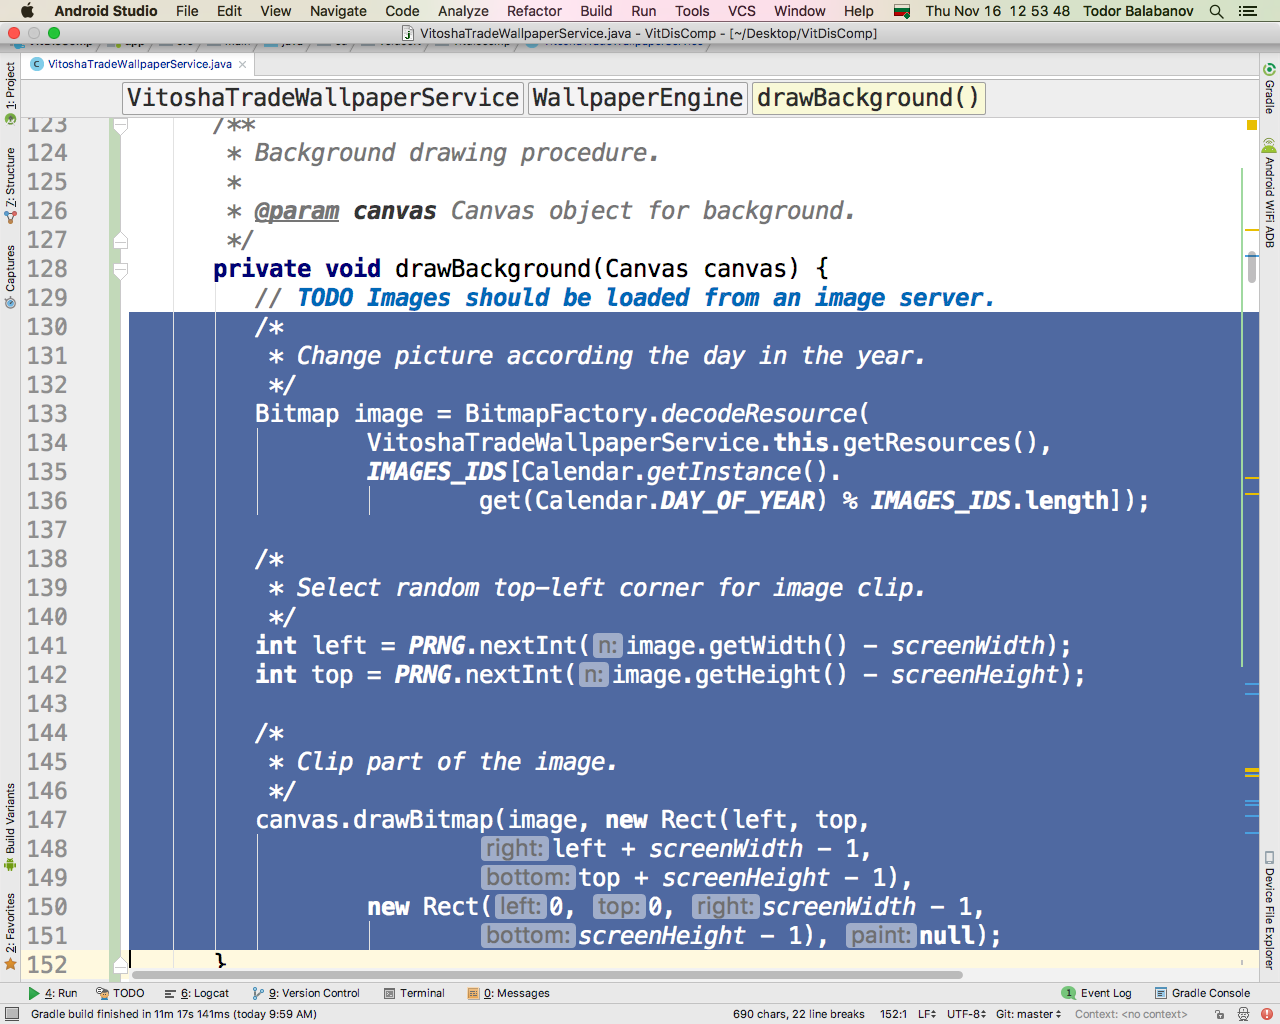
\includegraphics[height=0.45\pdfpageheight]{pic0052}
\caption{Paint the background}
\label{fig:pic0052}
\end{figure}
\FloatBarrier

A previously prepared image is loaded to draw the background, and a piece is cut from it to fit the screen's dimensions (Fig. \ref{fig:pic0052}). Which part of the image is used is determined randomly.

\begin{figure}[h]
\centering
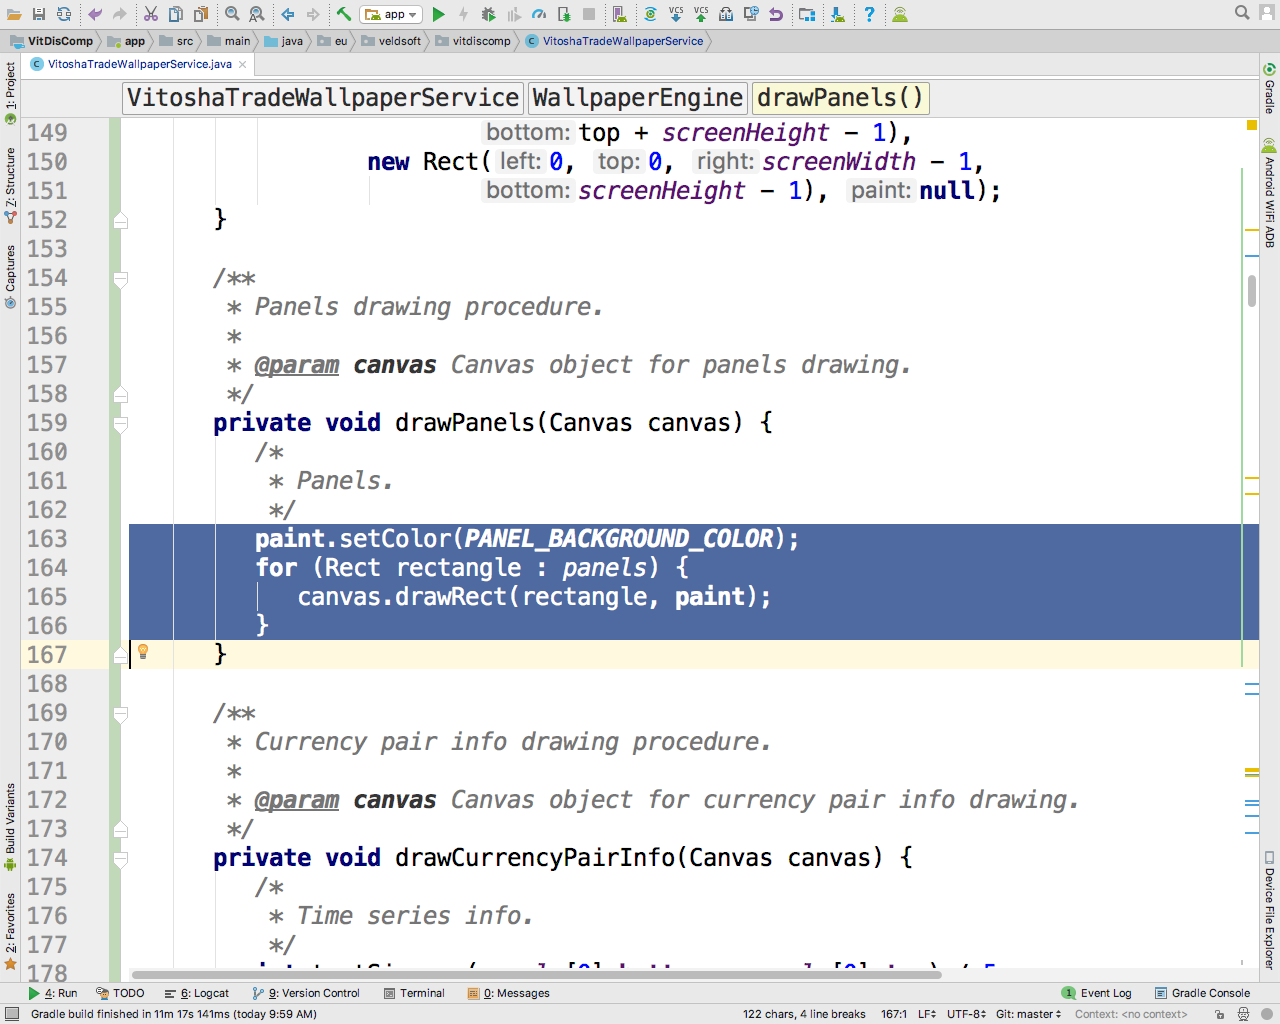
\includegraphics[height=0.45\pdfpageheight]{pic0053}
\caption{Drawing service information areas}
\label{fig:pic0053}
\end{figure}
\FloatBarrier

Immediately after drawing the background, the semi-transparent spots are also drawn to represent the information from the learning process visually (Fig. \ref{fig:pic0053}). A translucency grip is needed to avoid the side effect of color blending between the service information and the background.

\begin{figure}[h]
\centering
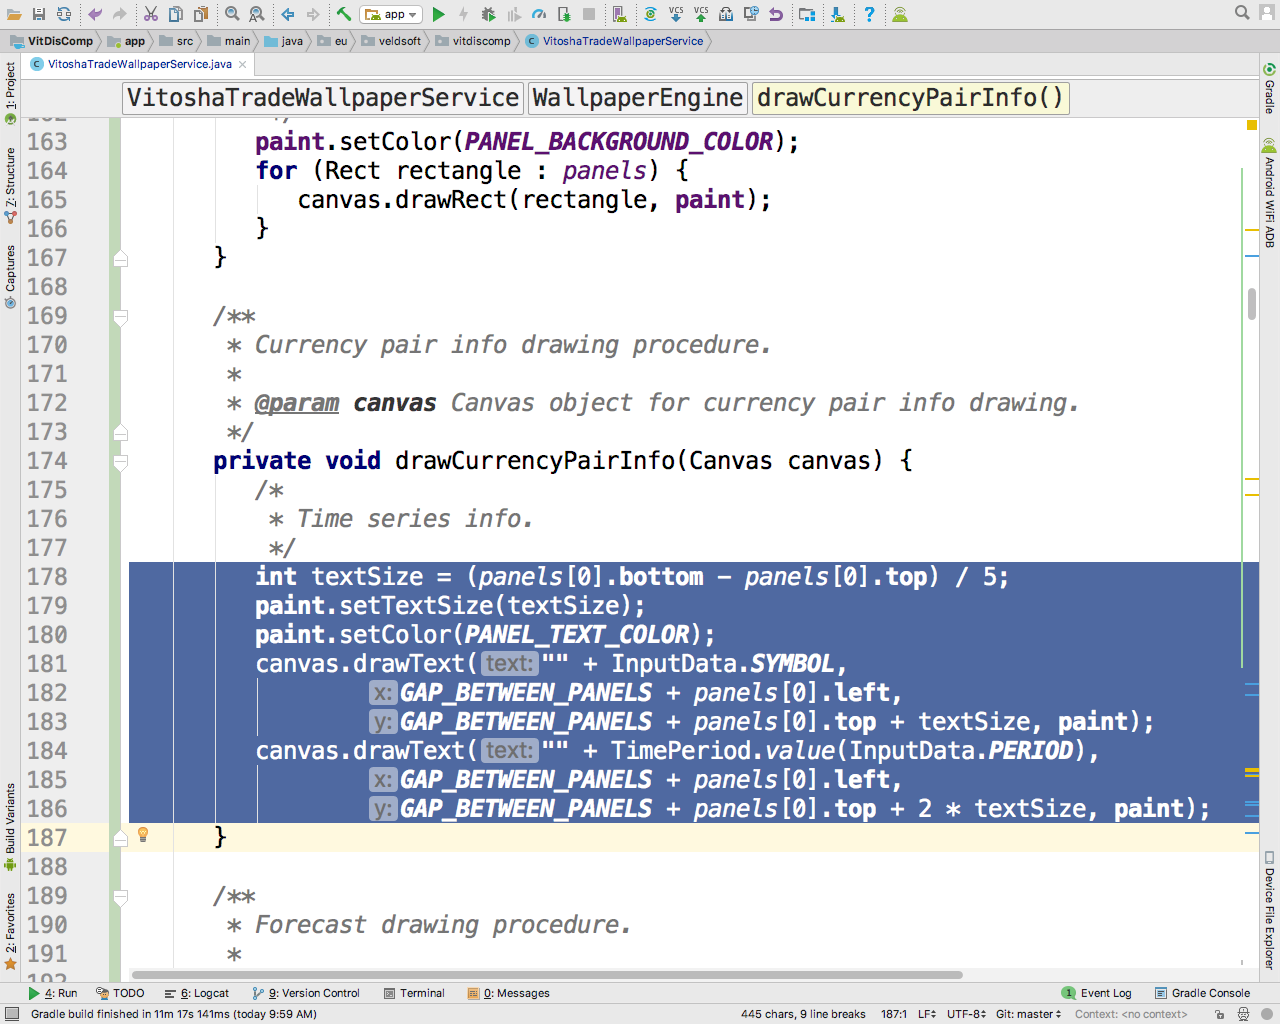
\includegraphics[height=0.45\pdfpageheight]{pic0054}
\caption{Drawing currency pair information}
\label{fig:pic0054}
\end{figure}
\FloatBarrier

The information about the currency pair consists of the name and time interval of the financial time series (Fig. \ref{fig:pic0054}).

\begin{figure}[h]
\centering
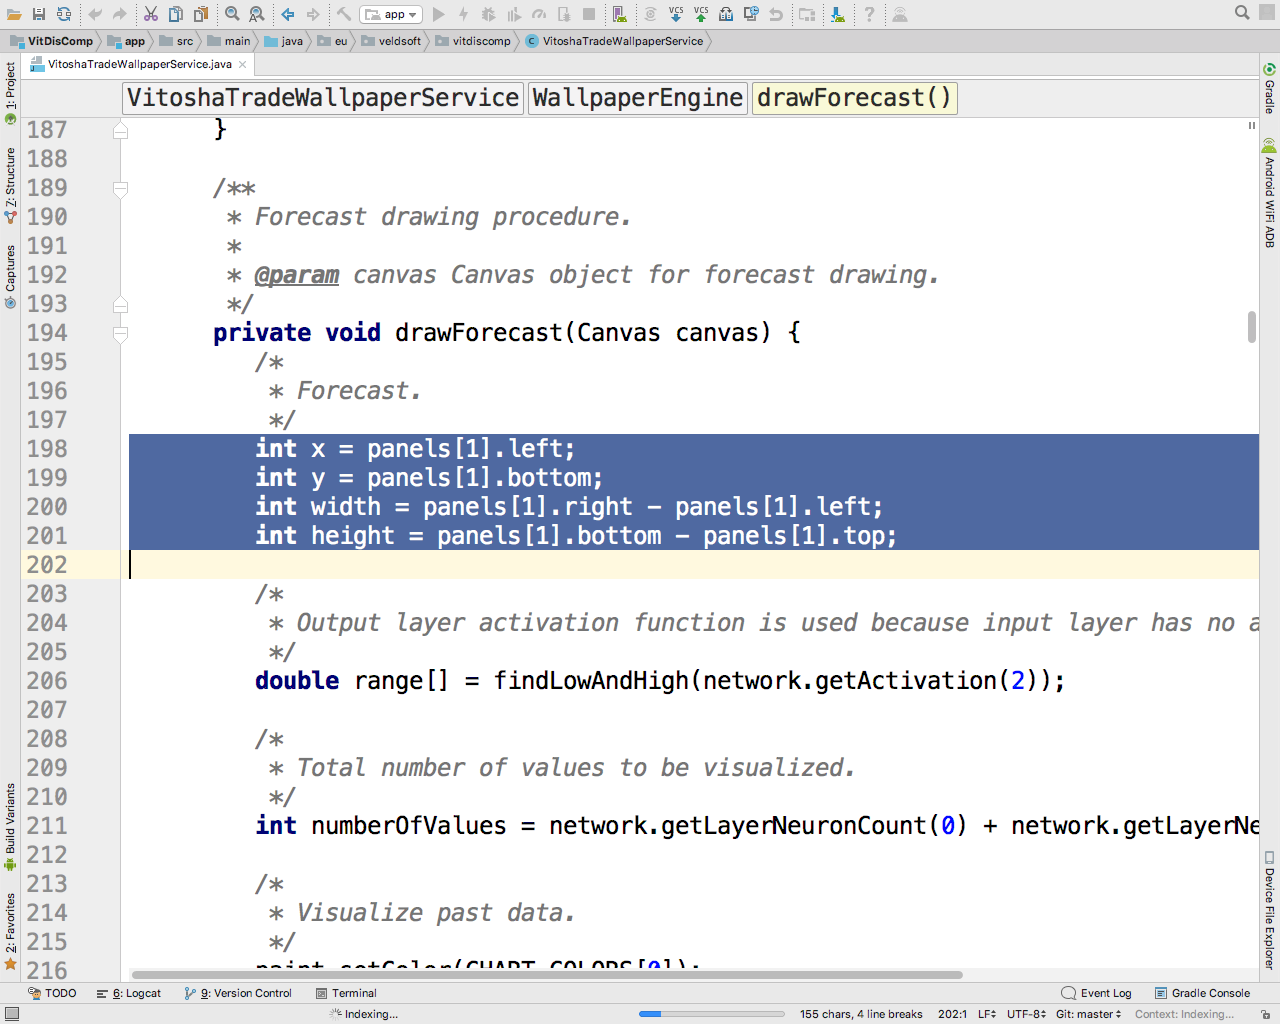
\includegraphics[height=0.45\pdfpageheight]{pic0055}
\caption{Position and dimensions for the visual representation of the forecast}
\label{fig:pic0055}
\end{figure}
\FloatBarrier

The visual representation of the prediction requires slightly more complex calculations so that the input and output information fit within the specified blob. To accomplish this task, the coordinates and dimensions of the specified area are taken (Fig. \ref{fig:pic0055}).

\begin{figure}[h]
\centering
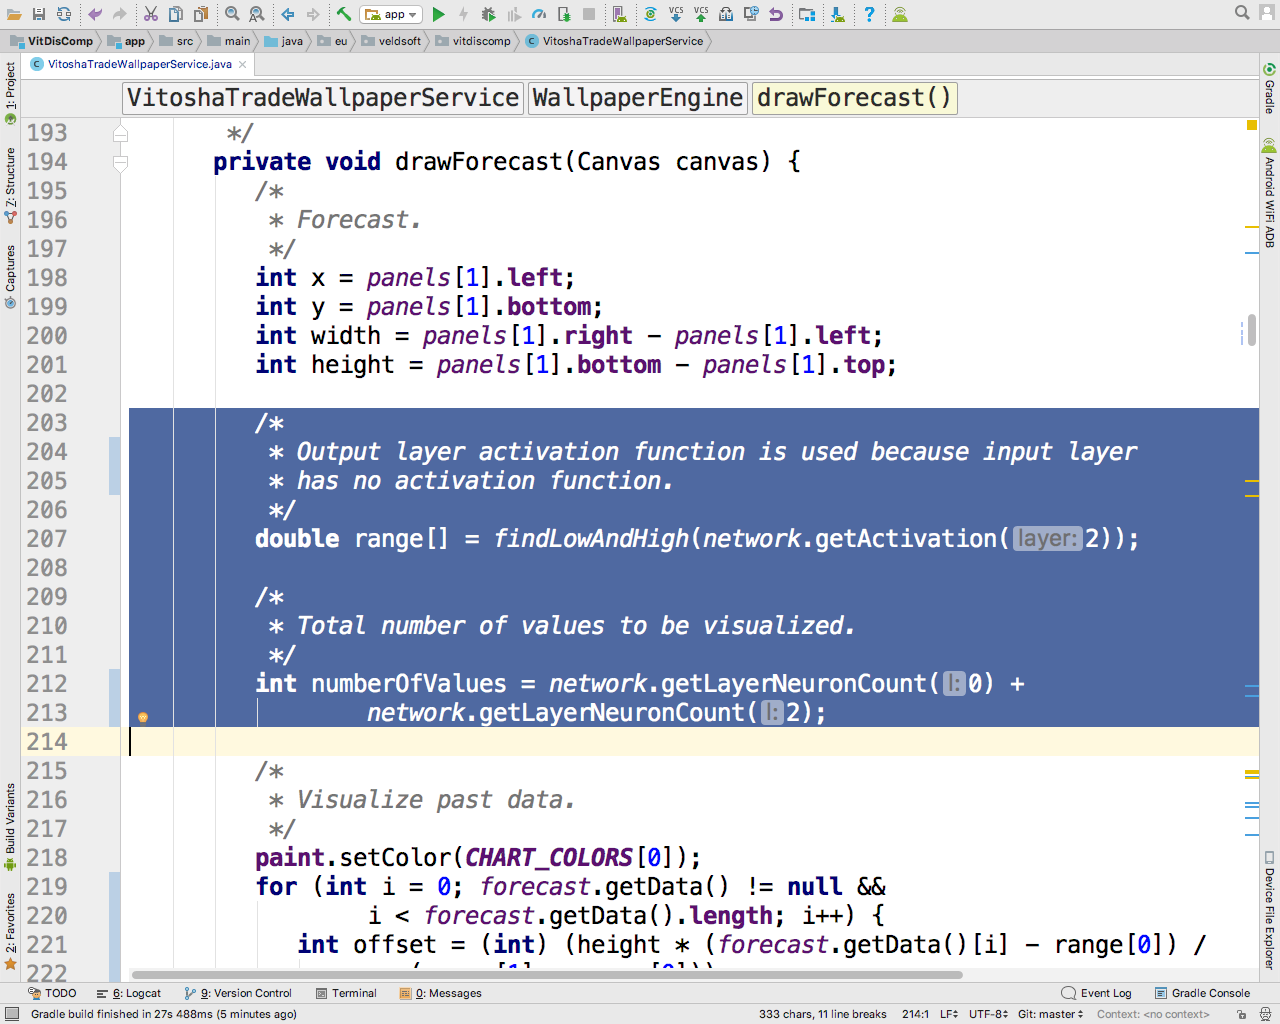
\includegraphics[height=0.45\pdfpageheight]{pic0056}
\caption{Width and height data range}
\label{fig:pic0056}
\end{figure}
\FloatBarrier

To visualize the data, it is essential to define the minimum and maximum values for the input-output as well as the number of values to be visualized (Fig. \ref{fig:pic0056}). In this case, the number of values for visual representation coincides with the sum of the number of input and the number of output signals.

\begin{figure}[h]
\centering
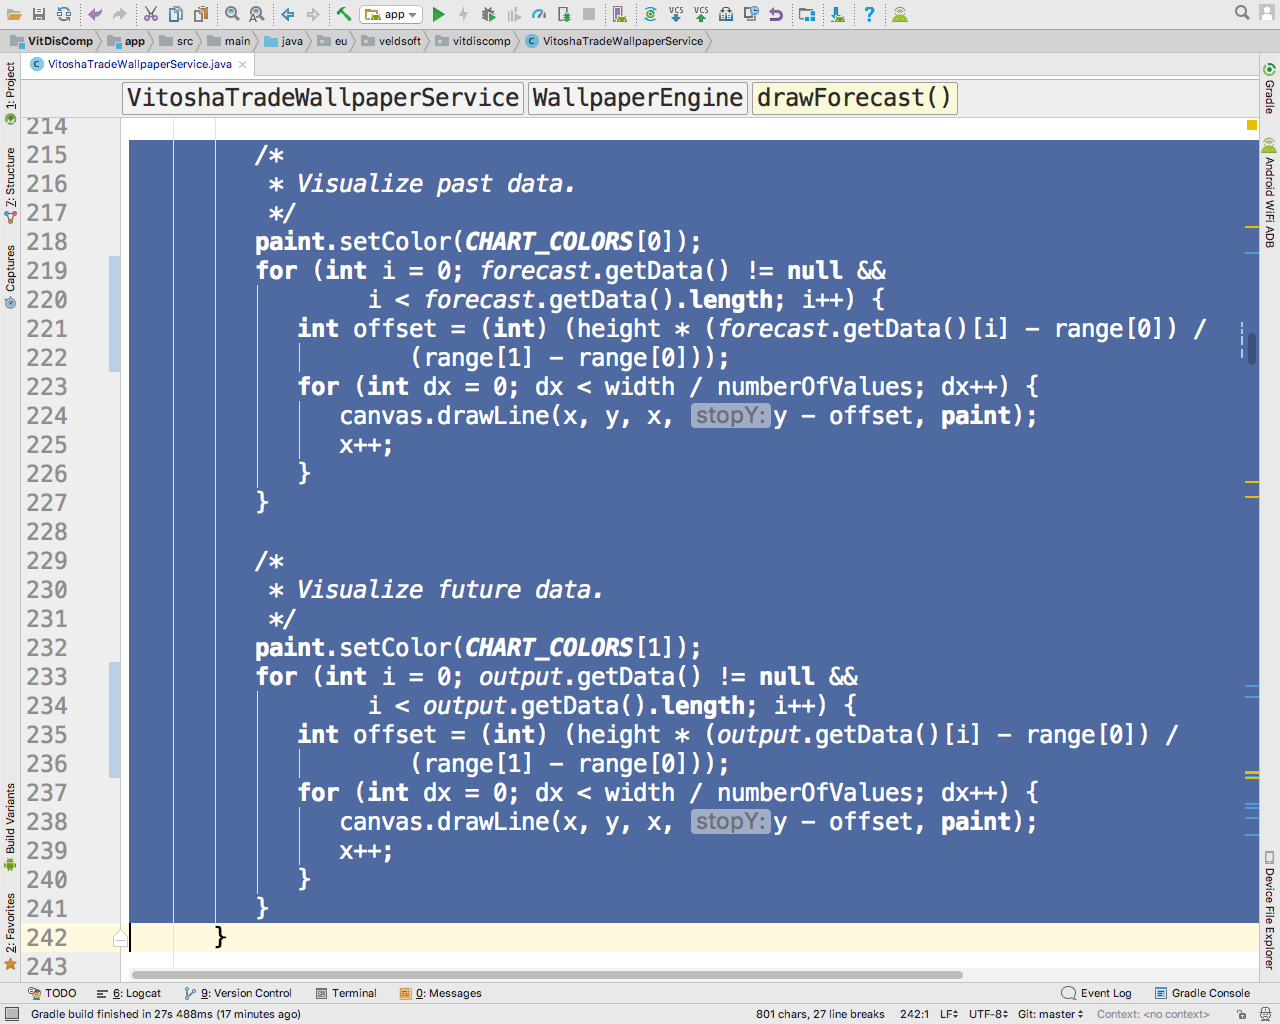
\includegraphics[height=0.45\pdfpageheight]{pic0057}
\caption{Cycles for visual presentation of the time series and forecast pillars}
\label{fig:pic0057}
\end{figure}
\FloatBarrier

The data for the elapsed period is shown in one color, and the forecast data in another color (Fig. \ref{fig:pic0057}). The visual presentation is a bar chart of the input data and the forecast.

\begin{figure}[h]
\centering
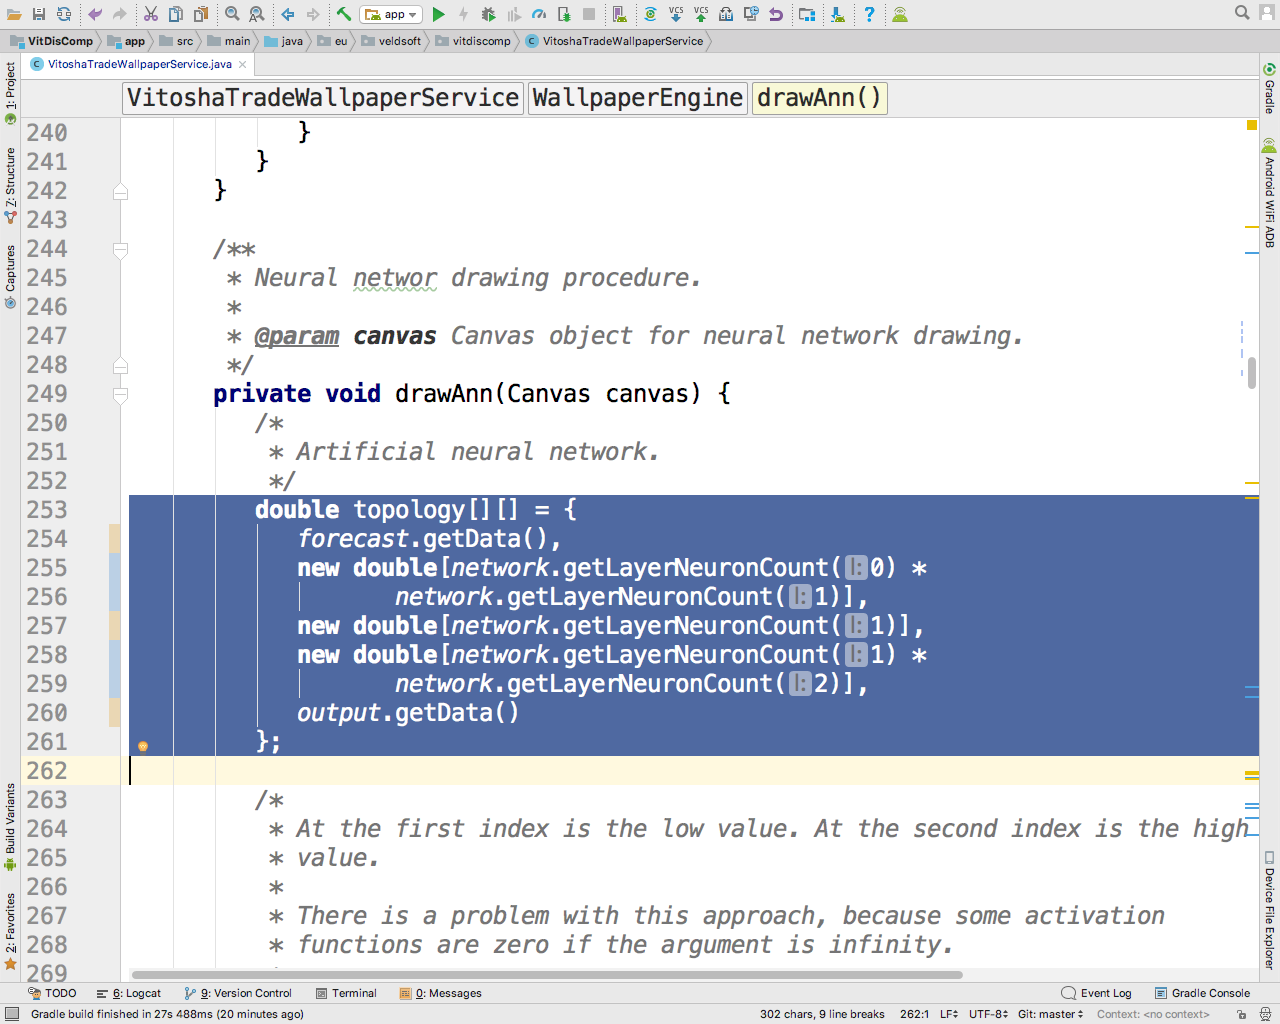
\includegraphics[height=0.45\pdfpageheight]{pic0058}
\caption{Topology of the artificial neural network being visualized}
\label{fig:pic0058}
\end{figure}
\FloatBarrier

In the third visual representation area, stylized information about the state of the artificial neural network is drawn\index{artificial neural networks}. The rectangular area is divided into five vertical zones: 1. Values of the neurons in the input layer; 2. Values of the weights between the input and the hidden layer; 3. Values of the neurons in the hidden layer; 4. Values of the weights between the hidden and output layers; 5. Values of neurons in the output layer (Fig. \ref{fig:pic0058}).

\begin{figure}[h]
\centering
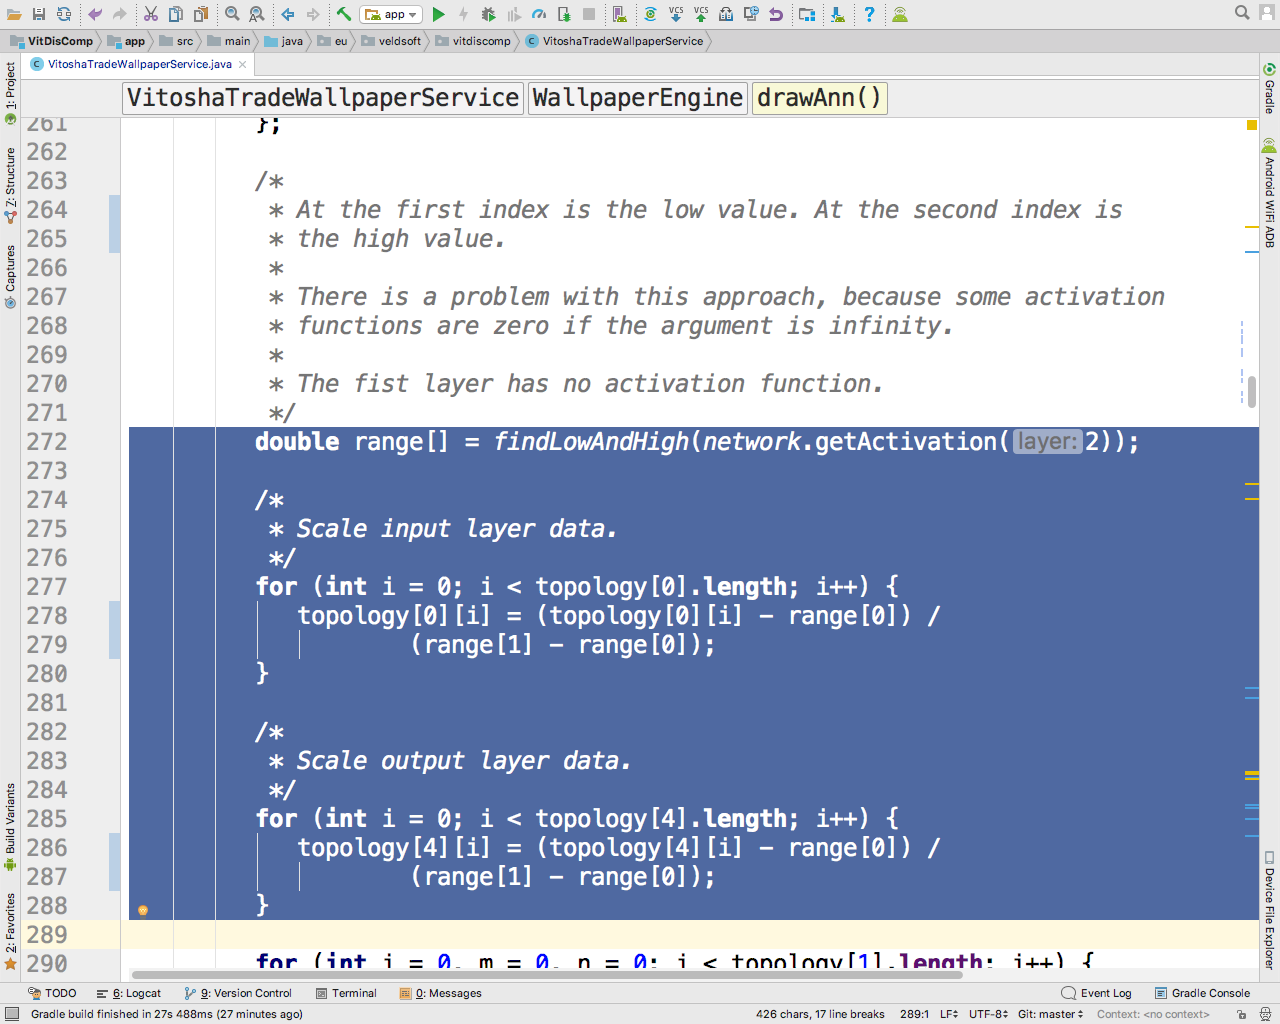
\includegraphics[height=0.45\pdfpageheight]{pic0059}
\caption{Input and output scaling}
\label{fig:pic0059}
\end{figure}
\FloatBarrier

The input and output information is resized relative to the minimum and maximum values that the neurons in the output layer work with (Fig. \ref{fig:pic0059}). The formula for MinMax Scaling (\ref{equation04}) is attached.

\begin{equation}
\label{equation04}
X_{sc} = \frac{X-X_{min}}{X_{max}-X_{min}}
\end{equation}

In practice, neurons in the input layer should not have an activation function constraint since they only collect information from the outside world.

\begin{figure}[h]
\centering
\includegraphics[height=0.45\pdfpageheight]{pic0060}
\caption{Weight values between layers}
\label{fig:pic0060}
\end{figure}
\FloatBarrier

Next is determining the weights between the layers (Fig. \ref{fig:pic0060}).

\begin{figure}[h]
\centering
\includegraphics[height=0.45\pdfpageheight]{pic0061}
\caption{Scaling the values in the hidden layer}
\label{fig:pic0061}
\end{figure}
\FloatBarrier

And finally, for the middle vertical region, the values for the hidden layer are determined and scaled to the minimum, and maximum level of the activation function applied to it (Fig. \ref{fig:pic0061}).

\begin{figure}[h]
\centering
\includegraphics[height=0.45\pdfpageheight]{pic0062}
\caption{Normalize values for weights}
\label{fig:pic0062}
\end{figure}
\FloatBarrier

To visualize the information about the weights, it is necessary to normalize their values relative to the smallest and largest value among them (Fig. \ref{fig:pic0062}).

\begin{figure}[h]
\centering
\includegraphics[height=0.45\pdfpageheight]{pic0063}
\caption{Draw the topology}
\label{fig:pic0063}
\end{figure}
\FloatBarrier

Thus, the previously prepared data is easily visualized by a group of nested loops (Fig. \ref{fig:pic0063}).

\begin{figure}[h]
\centering
\includegraphics[height=0.45\pdfpageheight]{pic0064}
\caption{Engine constructor for the service}
\label{fig:pic0064}
\end{figure}
\FloatBarrier

The service engine constructor has the sole task of loading the execution thread (Fig \ref{fig:pic0064}).

\begin{figure}[h]
\centering
\includegraphics[height=0.45\pdfpageheight]{pic0065}
\caption{Change in active wallpaper visibility}
\label{fig:pic0065}
\end{figure}
\FloatBarrier

When the visibility of the active wallpaper is changed, an onVisibilityChanged event is fired, which determines whether the thread should be reactivated or its calling terminated (Fig. \ref{fig:pic0065}).

\begin{figure}[h]
\centering
\includegraphics[height=0.45\pdfpageheight]{pic0066}
\caption{Stop calculations when destroying draw surface}
\label{fig:pic0066}
\end{figure}
\FloatBarrier

In the event of destroying the drawing area, a flag to stop the calculations is raised, and the thread responsible for them is removed from the execution queue (Fig. \ref{fig:pic0066}).

\begin{figure}[h]
\centering
\includegraphics[height=0.45\pdfpageheight]{pic0067}
\caption{Size of drawing areas}
\label{fig:pic0067}
\end{figure}
\FloatBarrier

When a change occurs in the drawing area of the active wallpaper, a series of resizing measures must be taken. Such an event, for example, occurs when the device changes the visual representation from portrait to landscape or vice versa. The first feature to monitor is the size of the spots for a graphical representation (Fig. \ref{fig:pic0067}).


\begin{figure}[h]
\centering
\includegraphics[height=0.45\pdfpageheight]{pic0068}
\caption{Coordinates and dimensions of visual representation areas - top-left}
\label{fig:pic0068}
\end{figure}
\FloatBarrier

\begin{figure}[h]
\centering
\includegraphics[height=0.45\pdfpageheight]{pic0069}
\caption{Coordinates and dimensions of visual representation areas - top-center}
\label{fig:pic0069}
\end{figure}
\FloatBarrier

\begin{figure}[h]
\centering
\includegraphics[height=0.45\pdfpageheight]{pic0070}
\caption{Coordinates and dimensions of visual representation areas - top-right}
\label{fig:pic0070}
\end{figure}
\FloatBarrier

\begin{figure}[h]
\centering
\includegraphics[height=0.45\pdfpageheight]{pic0071}
\caption{Coordinates and dimensions of visual representation areas - center-left}
\label{fig:pic0071}
\end{figure}
\FloatBarrier

\begin{figure}[h]
\centering
\includegraphics[height=0.45\pdfpageheight]{pic0072}
\caption{Coordinates and dimensions of visual representation areas - center-center}
\label{fig:pic0072}
\end{figure}
\FloatBarrier

\begin{figure}[h]
\centering
\includegraphics[height=0.45\pdfpageheight]{pic0073}
\caption{Coordinates and dimensions of visual representation areas - center-right}
\label{fig:pic0073}
\end{figure}
\FloatBarrier

\begin{figure}[h]
\centering
\includegraphics[height=0.45\pdfpageheight]{pic0074}
\caption{Coordinates and dimensions of visual representation areas - bottom-left}
\label{fig:pic0074}
\end{figure}
\FloatBarrier

\begin{figure}[h]
\centering
\includegraphics[height=0.45\pdfpageheight]{pic0075}
\caption{Coordinates and dimensions of visual representation areas - bottom-center}
\label{fig:pic0075}
\end{figure}
\FloatBarrier

\begin{figure}[h]
\centering
\includegraphics[height=0.45\pdfpageheight]{pic0076}
\caption{Coordinates and dimensions of visual representation areas - bottom-right}
\label{fig:pic0076}
\end{figure}
\FloatBarrier

The user can choose the part of the active wallpaper where the visual presentation areas should be positioned. The horizontal options are left, center, and right, and the vertical options are top, center, and bottom.

\begin{figure}[h]
\centering
\includegraphics[height=0.45\pdfpageheight]{pic0077}
\caption{System load for background calculations}
\label{fig:pic0077}
\end{figure}
\FloatBarrier

The final feature that the user can control is to what extent their mobile device will be loaded with background calculations (Fig. \ref{fig:pic0077}).

\section{Presentation of the information on the local device}

The efficiency of calculations is significantly increased if the local computing nodes can store source data and calculated results locally.

\begin{figure}[h]
\centering
\includegraphics[height=0.45\pdfpageheight]{pic0078}
\caption{Time series interval constants (0 to 15)}
\label{fig:pic0078}
\end{figure}
\FloatBarrier

For the needs of this local representation, an auxiliary data type of enumerated type is used, which indicates the distance between two readings in the financial time series (Fig. \ref{fig:pic0078}, \ref{fig:pic0079}).

\begin{figure}[h]
\centering
\includegraphics[height=0.45\pdfpageheight]{pic0079}
\caption{Constants for time series intervals (30 to 43200)}
\label{fig:pic0079}
\end{figure}
\FloatBarrier

The intervals in the time series are determined based on the number of minutes, with the shortest interval being one minute. The intervals are described with two variables - name and number of minutes (Fig. \ref{fig:pic0080}).

\begin{figure}[h]
\centering
\includegraphics[height=0.45\pdfpageheight]{pic0080}
\caption{Time slot description}
\label{fig:pic0080}
\end{figure}
\FloatBarrier

The use of enumerated constants in Java makes it possible to elegantly use static functions to construct objects (Factory Method Design Pattern) that, after a given number (number of minutes), return the corresponding constant (Fig. \ref{fig:pic0081}).

\begin{figure}[h]
\centering
\includegraphics[height=0.45\pdfpageheight]{pic0081}
\caption{Defining an interval constant by number of minutes}
\label{fig:pic0081}
\end{figure}
\FloatBarrier

A similar effect can be achieved using the text description of the constants (Fig. \ref{fig:pic0082}).

\begin{figure}[h]
\centering
\includegraphics[height=0.45\pdfpageheight]{pic0082}
\caption{Defining an interval constant by textual description}
\label{fig:pic0082}
\end{figure}
\FloatBarrier

To prevent the creation of constants outside the enumerated type, it is assumed that the constructor has a private access level (Fig. \ref{fig:pic0083}).

\begin{figure}[h]
\centering
\includegraphics[height=0.45\pdfpageheight]{pic0083}
\caption{Constructor of the enumerated type for space}
\label{fig:pic0083}
\end{figure}
\FloatBarrier

The Android operating system provides reasonable means of storing information, including the SQLite relational database management system.

\begin{figure}[h]
\centering
\includegraphics[height=0.45\pdfpageheight]{pic0084}
\caption{Local table structure for quotations}
\label{fig:pic0084}
\end{figure}
\FloatBarrier

Information about the time series can be stored locally in a table with a suitable structure that reflects the presence of four values for each interval, the time of the interval, the traded volume, the name of the currency pair, and the size of the time interval (Fig. \ref{fig:pic0084}).

\begin{figure}[h]
\centering
\includegraphics[height=0.45\pdfpageheight]{pic0085}
\caption{Local Table Structure for Artificial Neural Networks}
\label{fig:pic0085}
\end{figure}
\FloatBarrier

An additional table takes care of the storage of the information about the artificial neural networks, which includes the name of the currency pair, the time interval, the value of the neurons, the value of the connections between the neurons, and the value of the weights between the neurons (Fig. \ref{fig:pic0085}).

\begin{figure}[h]
\centering
\includegraphics[height=0.45\pdfpageheight]{pic0086}
\caption{Database name and version}
\label{fig:pic0086}
\end{figure}
\FloatBarrier

Android manages databases in the form of a DB resource and an integer version for the structure (Fig. \ref{fig:pic0086}).

\begin{figure}[h]
\centering
\includegraphics[height=0.45\pdfpageheight]{pic0087}
\caption{Code to create the quote table}
\label{fig:pic0087}
\end{figure}
\FloatBarrier

\begin{figure}[h]
\centering
\includegraphics[height=0.45\pdfpageheight]{pic0088}
\caption{Code to create the artificial neural network table}
\label{fig:pic0088}
\end{figure}
\FloatBarrier

Parameterized symbolic constants control the creation of the tables (Fig. \ref{fig:pic0087}, \ref{fig:pic0088}).

\begin{figure}[h]
\centering
\includegraphics[height=0.45\pdfpageheight]{pic0089}
\caption{Code to delete the tables}
\label{fig:pic0089}
\end{figure}
\FloatBarrier

Deleting tables is also done with parameterized symbolic constants (Fig. \ref{fig:pic0089}).

\begin{figure}[h]
\centering
\includegraphics[height=0.45\pdfpageheight]{pic0090}
\caption{Constructor and virtual methods of the database helper class}
\label{fig:pic0090}
\end{figure}
\FloatBarrier

The constructor of the helper class for the database has the sole task of calling the parent class's constructor (Fig \ref{fig:pic0090}). The two predefined virtual functions call the requests to construct and update the database (Fig. \ref{fig:pic0090}).

\begin{figure}[h]
\centering
\includegraphics[height=0.45\pdfpageheight]{pic0091}
\caption{Type listed for neuron type}
\label{fig:pic0091}
\end{figure}
\FloatBarrier

The second type of data listed is regarding the type of neurons. In general, neurons can be regular, input, output, and bias (Fig. \ref{fig:pic0090}).

\begin{figure}[h]
\centering
\includegraphics[height=0.45\pdfpageheight]{pic0092}
\caption{An integer constant for the neuron type that can also be used as a bit field}
\label{fig:pic0092}
\end{figure}
\FloatBarrier

Since different connections between neurons are possible, neurons with more functions appear, such as: regular-input, regular-output, input-output, and input-regular-output. All possible combinations are recorded in an integer variable, which can also serve as a bit field (Fig. \ref{fig:pic0092}).

\begin{figure}[h]
\centering
\includegraphics[height=0.45\pdfpageheight]{pic0093}
\caption{Determining the enumerable constant by numeric value}
\label{fig:pic0093}
\end{figure}
\FloatBarrier

Since the information from the server arrives mainly in the form of numbers, it is rational to add a static function for constructing the object (Factory Method Design Pattern), which numerically determines the constant in the enumerated type (Fig. \ref{fig:pic0093}).

\begin{figure}[h]
\centering
\includegraphics[height=0.45\pdfpageheight]{pic0094}
\caption{Methods to access constant internal values}
\label{fig:pic0094}
\end{figure}
\FloatBarrier

For convenience, accessor methods are often used when working with constants and the information hidden in them. In this case, a public getter but a setter with private access. It makes sense to make the setter private to preserve the property of enumerated constants to stay constants (Fig \ref{fig:pic0094}).
